\documentclass[10pt, mathserif]{beamer}
\include{custom}


\title[Contributions to FE Analysis in Electromagnetics]{\textsf{\Large{{Contributions to the Art of Finite Element Analysis in Electromagnetics}}}}
\author[Laurent Ntibarikure]{} 
\date[\today]{}
\institute[University of Florence]{}
\subject{Finite Element Analysis in Electromagnetics}


\begin{document}
%%%%% PRIMA PAGINA
\frame{
\begin{center}

\includegraphics[width=3cm]{LOGOUNIFI.pdf} \\
%\vspace{-0.1cm}\textsl{\scriptsize{Universit\`{a} degli Studi di Firenze}}\\%\\[-0.1cm]Departimento di Elettronica e Telecomunicazioni}}\\[0.5cm]
\small{Dottorato di Ricerca in\\Tecnologie Elettroniche per l'Ingegneria dell'Informazione\\Indirizzo \emph{``RF, Microwaves and Electromagnetics''}\\ Ciclo XXVI}
\end{center}
\vspace{-.1cm}{\maketitle}
\begin{center}
\vspace{-2.5cm} Laurent Ntibarikure \\[-3cm]
\end{center}
\vspace{-1cm}
\begin{table}[h]
\begin{tabular*}{\textwidth}[b]{rlll}
%\hspace{-.5cm} 
%\includegraphics[width=1cm]{unifiLogo.pdf} \hspace{0.2cm} & & & %\hspace{-0.6cm} 
%& \hspace{-0.2cm} \scriptsize{Relatori:} & \hspace{-0.1cm}  \scriptsize{Relatori esterni:} & \\[.15cm]
%& \scriptsize{Prof. Giuseppe Pelosi} & \hspace{0cm} \scriptsize{Prof. Romanus Dyczij-Edlinger} &\\
%& \scriptsize{Dr. Ing. Stefano Selleri} & \hspace{0cm} \scriptsize{Dr. Ing. Ortwin Farle} &
\end{tabular*}
\end{table}
\begin{center}
\vspace{-.5cm}
\footnotesize{2010-2013}
\end{center}
}

%%%%%% SUMMARY
%\section*{Summary}
%\frame{\tableofcontents}
%
%%%%% MOTIVAZIONI

\section{Introduction}

\subsection{Large electromagnetic problems}
\frame
{
\frametitle{Large electromagnetic problems}
\begin{block}{}
\quotes{Traditional} methods such as FE, FDTD and MoM fail due to high computational resources requirements
\end{block}
\begin{block}{}
Seek for efficient solvers relying on domain decomposition methods
%%\only<1>{
%\begin{itemize}
%\item Multigrid methods
%\item Domain decomposition methods
%\item Multipole methods
%\end{itemize}	
\end{block}
%}
%\only<2>{
%\begin{itemize}
%\item Multigrid methods
%\item \alert{Domain decomposition methods}
%\item Multipole methods
%\end{itemize}	
%\end{block}
%}
}

\subsection{Nonlinear materials analyzes}
\frame
{
\frametitle{Nonlinear materials analyzes}
\begin{block}{}
\begin{itemize}
\item Material properties ($\dyad{\epsilon}$, $\dyad{\mu}$, $\dyad{\sigma}$) depend on field intensities
\item Higher order harmonics are generated
\end{itemize}	
\end{block}
\begin{block}{}
Frequency domain analysis needs for multiple harmonics formulation
\end{block}
}


\frame{
\frametitle{Outline}
\begin{enumerate}
\item Finite Element Software (FES) implementation in C++ and validation with commercial packages
\item Investigation of finite element domain decomposition methods and their computational efficiencies
\item Introduction of multiharmonic finite element formulation for the time-harmonic wave equation
\end{enumerate}
}

\section{Finite elements for electromagnetics}
\subsection{Radiation in an unbounded medium}
\frame{
\frametitle{Radiation in an unbounded medium}
Time-harmonic Maxwell's equations $\left(\mathbf{E} \leftrightarrow \mathfrak{Re} \left\lbrace {\mathcalb{E}} \mathrm{e}^{j\omega t} \right\rbrace \right)$
\begin{eqnarray}
\nabla \times {\mathbf{E}} &= & -j\omega{\mathbf{B}}\label{eq:ffaraday} \\
\nabla \times {\mathbf{H}} &= & j\omega{\mathbf{D}} +  \dyad{\sigma} \mathbf{E} +{\mathbf{J}^i} \label{eq:fampere} \\
\nabla \cdot {\mathbf{D}} &= & {\rho}\label{eq:fpoisson}\\
\nabla \cdot {\mathbf{B}} &= & 0\label{eq:fgauss}
\end{eqnarray}
Medium constitutive relations
\begin{eqnarray} 
{\mathbf{D}} &= & \epsilon_0 \dyad{\epsilon}_r {\mathbf{E}}  \label{eq:ffsconst1}\\
{\mathbf{B}} &= & \mu_0 \dyad{\mu}_r {\mathbf{H}} \label{eq:ffsconst2}
\end{eqnarray}

}

\frame{
\frametitle{Wave equation}
Upon combining the curl of Faraday's equation \eqref{eq:ffaraday}, Amp\`ere's law \eqref{eq:fampere} and the constitutive relation \eqref{eq:ffsconst2}
\begin{eqnarray*}
\nabla \times \frac{1}{\dyad{\mu}_r} \nabla \times {\mathbf{E}} + j k_0 \zeta_0 \dyad{\sigma} {\mathbf{E}} - k_0^2 \dyad{\epsilon}_r {\mathbf{E}} &= & 0 \label{eq:waveeqE}
\end{eqnarray*}
The wave equation in the electric field describes electromagnetic fields propagation, and the magnetic field $\mathbf{H}$ is tightly bound to the electric field and material properties
\begin{eqnarray*}
{\mathbf{H}} &= & \frac{\nabla \times {\mathbf{E}}}{-j k_0\zeta_0\dyad{\mu}_r}  \label{eq:waveeqErecH}
\end{eqnarray*}
}


\subsection{Finite element method}
\frame{
\frametitle{Finite element method}
\begin{block}{}
A partial differential equation (PDE), say the wave equation, describes the physics of the problem
\end{block}
\begin{block}{}
Finite elements consists of a robust numerical procedure for solving the equation
\begin{itemize}
\item Preprocessing
\item Assembly
\item Solution
\item Postprocessing
\end{itemize}
\end{block}
}

\graphicspath{{img/ch1/}}

\frame{
\frametitle{Preprocessing}
\begin{itemize}
\item Numerical (CAD) model of the domain $\Omega$ of analysis
\begin{columns}
\begin{column}{5cm}
\begin{itemize}
\item Material properties definition
\item Boundary conditions for domain truncation
\end{itemize} 
\end{column}
\begin{column}{3cm}
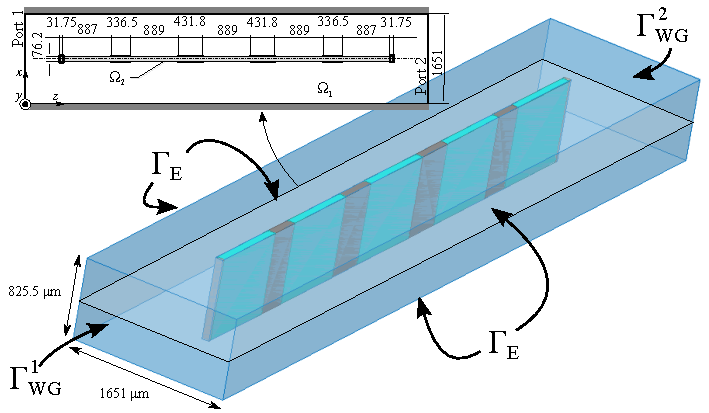
\includegraphics[width=3.5cm]{Bui1984}
\end{column}
\end{columns}
\item Definition of the function space
\item Selection of local basis functions on simple subdomains, the elements of the mesh $\mathcal{M}_h(\Omega)$
\begin{center}
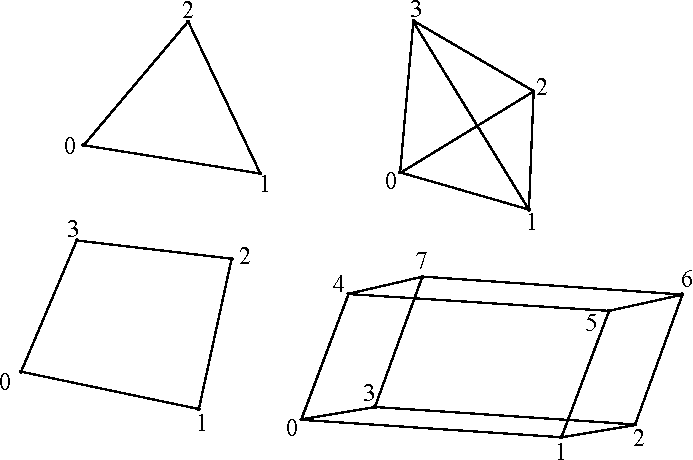
\includegraphics[width=4cm]{Elements} \ \ \ 
\includegraphics[width=4cm]{Mesh}
\end{center}
\item Problem model formulation based on the physics
\end{itemize}

}


\frame{
\frametitle{Preprocessing : Function spaces for electromagnetic quantities}

We need to define``bounded'' spaces to ensure convergence of the solution to the exact solution (Cae's theorem) : \underline{Sobolev spaces}
\begin{table}[h!]
\begin{center}
\begin{tabular}{|c|c|}
\hline 
Quantity & Function space \\ 
\hline
\hline 
$\mathbf{E}, \mathbf{H}$ & $\mathcal{H}(\mathrm{curl},\Omega)$ \\ 
\hline 
$\mathbf{D}, \mathbf{B}, \mathbf{J}$ & $\mathcal{H}(\mathrm{div},\Omega)$ \\ 
\hline 
$\rho$ & $\mathcal{L}^2(\Omega)$ \\ 
\hline 
$\epsilon_0 \dyad{\epsilon}_r, \mu_0 \dyad{\mu}_r$ & $\mathcal{H}(\mathrm{curl},\Omega) \longrightarrow \mathcal{H}(\mathrm{div},\Omega)$ \\ 
\hline 
\end{tabular}
\end{center}
\label{tab:quantspace}
\end{table}
Strong relationship between spaces : \underline{de Rham complex}
$$\mathcal{H}^1(\Omega) \ \stackrel{\nabla}{  \longrightarrow} \ \mathcal{H}(\mathrm{curl},\Omega) \ \stackrel{ \nabla\times}{ \longrightarrow} \ \mathcal{H}(\mathrm{div},\Omega) \stackrel{\nabla\cdot}{ \longrightarrow} \ \mathcal{L}^2(\Omega)$$
}


\frame{
\frametitle{Preprocessing : Scalar basis functions on triangle or tetrahedra}

$\mathcal{H}^1(\Omega)$ space is expanded by simplex coordinates $\phi_i$ (the continuous function that is linear on each triangle or tetrahedron, being one at node $i$ and zero at all other nodes)

\begin{table}[h!]
\begin{center}
\begin{tabular}{|c|c|c|}
\hline 
Space & Basis functions & Mesh entity \\ 
\hline
\hline 
$\mathcal{S}^1$ & $\phi_i$ & $\lbrace i \rbrace$ \\ 
\hline 
$\mathcal{S}^2$ & $\phi_i\phi_j$ & $\lbrace ij \rbrace$ \\ 
\hline 
$\mathcal{S}^3$ & $\phi_i\phi_j(\phi_i - \phi_j)$ & $\lbrace ij \rbrace$ \\ 
 & $\phi_i\phi_j\phi_k$ & $\lbrace ijk \rbrace$ \\ 
\hline 
\end{tabular} 
\end{center}
%\caption{$\mathcal{H}^1(\Omega)$-conforming basis functions up to order $p = 3$.}
\label{tab:H1functions}
\end{table}

\centering
$\mathcal{V}^p := \mathcal{S}^1 \oplus \ldots \oplus \mathcal{S}^p$, where $\mathcal{S}^p \subset \mathcal{H}^1(\Omega)$

}

\frame{
\frametitle{Preprocessing : Rotational basis functions on triangle or tetrahedra}
$\mathcal{H}(\mathrm{curl},\Omega)$ is expanded with N\'ed\'elec's incomplete order spaces
\begin{table}[h!]
\begin{center}
\begin{tabular}{|c|c|c|}
\hline 
Space & Basis functions & Mesh entity \\
\hline
\hline 
$\mathcal{R}^1$ & $\phi_i\nabla\phi_j-\phi_j\nabla\phi_j$ & $\lbrace ij \rbrace$ \\
\hline 
$\mathcal{R}^2$ & $3\phi_j\phi_k\nabla\phi_i-\nabla(\phi_i\phi_j\phi_k)$ & $\lbrace ijk \rbrace$ \\
 & $3\phi_k\phi_i\nabla\phi_j-\nabla(\phi_i\phi_j\phi_k)$ & $\lbrace ijk \rbrace$ \\
\hline 
$\mathcal{R}^3$ & $4\phi_j\phi_k(\phi_j - \phi_k)\nabla\phi_i - \nabla\left(\phi_i\phi_j\phi_k(\phi_j-\phi_k)\right)$ & $\lbrace ijk \rbrace$ \\
 & $4\phi_k\phi_i(\phi_k - \phi_i)\nabla\phi_j - \nabla\left(\phi_i\phi_j\phi_k(\phi_k-\phi_i)\right)$ & $\lbrace ijk \rbrace$ \\
 & $4\phi_i\phi_j(\phi_i - \phi_j)\nabla\phi_k - \nabla\left(\phi_i\phi_j\phi_k(\phi_i-\phi_j)\right)$ & $\lbrace ijk \rbrace$ \\
 & $4\phi_j\phi_k\phi_l\nabla\phi_i - \nabla(\phi_i\phi_j\phi_k\phi_l)$ & $\lbrace ijkl \rbrace$ \\ 
 & $4\phi_k\phi_l\phi_i\nabla\phi_j - \nabla(\phi_i\phi_j\phi_k\phi_l)$ & $\lbrace ijkl \rbrace$ \\ 
 & $4\phi_l\phi_i\phi_j\nabla\phi_k - \nabla(\phi_i\phi_j\phi_k\phi_l)$ & $\lbrace ijkl \rbrace$ \\ 
\hline 
\end{tabular} 
\end{center}
%\caption{$\mathcal{H}(\mathrm{curl},\Omega)$-conforming basis functions up to order $p = 3$.}
\label{tab:Hcurlfunctions}
\end{table}
%
\centering
$\mathcal{W}^p = \mathcal{W}^{p-1} \oplus \bar{\mathcal{W}}^{p}$ for $ p = 2, 3$  and $\mathcal{W}^{1}= \mathcal{R}^{1}$, $\bar{\mathcal{W}}^p = \mathcal{R}^p \oplus \nabla \mathcal{S}^p$
}

\frame{
\frametitle{Preprocessing : Problem model for electromagnetic radiation}
\begin{center}
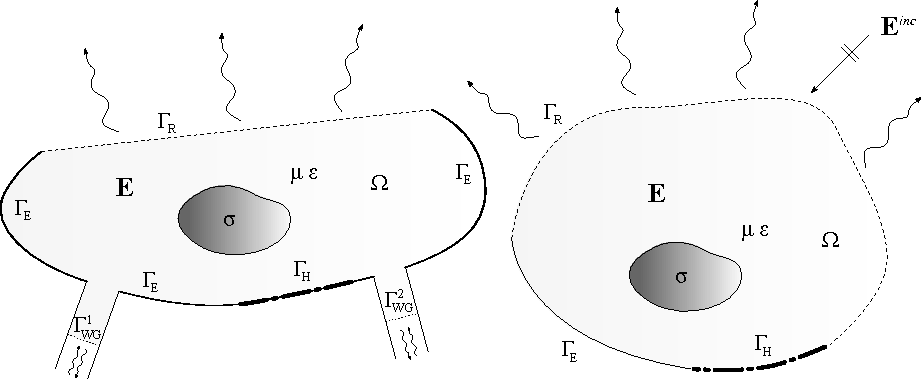
\includegraphics[width=10cm]{FEMproblem} 
\end{center}
Let us consider the domain $\Omega \subset \mathbb{R}^3$ to be bounded by
\begin{itemize}
\item $\mathrm{\partial \Omega = \Gamma = \Gamma_E \cup \Gamma_{H} \cup \Gamma_{WG} \cup \Gamma_R}$ in the antenna problem
\item $\mathrm{\partial \Omega = \Gamma = \Gamma_E \cup \Gamma_{H} \cup \Gamma_R}$ for the scattering problem
\end{itemize}
We seek for $\mathbf{E}$ that satisfies 
\begin{center}
$\nabla \times \frac{1}{\mu_r} \nabla \times \mathbf{E} + j k_0 \zeta_0 \sigma {\mathbf{E}} - k_0^2 \epsilon_r {\mathbf{E}} =  0$ in $\Omega$
\end{center}
}

\frame{
\frametitle{Preprocessing : Galerkin framework}
Curl-conforming shape functions $\mathbf{w} \in \mathcal{W} = \mathcal{W}(\Omega_h) \subset \mathcal{H}(\mathrm{curl}, \Omega)$
%These allow to consider vanishing tangential fields on $\Gamma_E$
\begin{eqnarray*}
\mathcal{W}_E &:= & \{ \mathbf{w} \in \mathcal{W} \ | \ \hat{\mathbf{n}} \times \mathbf{w} = 0 \ \text{on} \ \Gamma_E \} \subset \mathcal{H}(\mathrm{curl},\Omega, \Gamma_E)\nonumber
\end{eqnarray*}
\begin{center}
$\hat{\mathbf{n}}$ outwardly directed from $\Omega$
\end{center}
\underline{Electric field expansion}: 
$$\mathbf{E} := \sum_{j=1}^{N} x_j \mathbf{w}_j, \quad \mathbf{w}_j \in \mathcal{W}_E$$
\underline{Galerkin projection}: $$ \int_\Omega \mathbf{w}_i^* \cdot \left ( \nabla \times \frac{1}{\mu_r} \nabla \times {\mathbf{E}} + j k_0 \zeta_0 \sigma {\mathbf{E}} - k_0^2 \epsilon_r {\mathbf{E}} \right) d\Omega =  0$$
$$\Downarrow$$
$$\mat{A} \ \vect{x}   =  \vect{b}$$
$\mat{A} \in \mathbb{C}^{N \times N}$, $\vect{x}$ and $\vect{b} \in \mathbb{C}^{N}$
}

\frame{
\frametitle{Preprocessing : Boundary conditions}
\begin{itemize}
\item Perfect electric and magnetic conductors
\begin{eqnarray*}
\hat{\mathbf{n}} \times ( {\mathbf{E}} \times \hat{\mathbf{n}}) & = & 0,  \quad \text{on} \ \mathrm{\Gamma}_E \\
\hat{\mathbf{n}} \times ( {\mathbf{H}} \times \hat{\mathbf{n}}) & = & 0, \quad  \text{on} \ \mathrm{\Gamma}_H
\end{eqnarray*}
\item Radiation (with external impinging field if imposed)
\begin{eqnarray*}
\label{eq:IncBnd}
\hat{\mathbf{n}} \times \mathbf{H} & = & \frac{1}{Z_s} \hat{\mathbf{n}} \times \hat{\mathbf{n}} \times \mathbf{E} +\nonumber\\  & & \hspace{-2cm} \left( \hat{\mathbf{n}} \times \mathbf{H}^{inc} - \frac{1}{Z_s} \hat{\mathbf{n}} \times \hat{\mathbf{n}} \times \mathbf{E}^{inc} \right), \quad \text{on} \ \Gamma_{R}
\end{eqnarray*}
\end{itemize}
}

\frame{
\frametitle{Preprocessing : Boundary conditions}
\begin{itemize}
\item Dominant mode continuity on waveports
\begin{equation*}
\label{eq:WGcond}
\hat{\mathbf{n}} \times \mathbf{H}_t^k = \frac{1}{Z_k} \hat{\mathbf{n}} \times \hat{\mathbf{n}} \times \mathbf{E}_t^k - \frac{2}{Z_k} \hat{\mathbf{n}} \times \hat{\mathbf{n}} \times \mathbf{E}_t^{k \ inc}, \quad \text{on} \ \Gamma_{WG}^k
\end{equation*}
\item Transfinite elements on waveports
\begin{equation*}
\left\{
\begin{aligned}
\hat{\mathbf{n}} \times ( {\mathbf{E}} \times \hat{\mathbf{n}}) & = &  \sum_{k} \left ( a_k^r + a_k^i \right ) \mathbf{E}_t^k, \quad \text{on} \ \mathrm{\Gamma}_{WG}\\
\hat{\mathbf{n}} \times ( {\mathbf{H}} \times \hat{\mathbf{n}}) & = &  \sum_{k} \left ( a_k^r - a_k^i \right ) \mathbf{H}_t^k, \quad \text{on} \ \mathrm{\Gamma}_{WG}
\end{aligned}
\right.
\end{equation*}
\end{itemize}
}


\frame{
\frametitle{Preprocessing : Dominant mode continuity in antenna problem -- weak form}
$$ \int_\Omega \mathbf{w}_i^* \cdot \left ( \nabla \times \frac{1}{\mu_r} \nabla \times {\mathbf{E}} + j k_0 \zeta_0 \sigma {\mathbf{E}} - k_0^2 \epsilon_r {\mathbf{E}} \right) d\Omega =  0$$
$$\Downarrow$$
\begin{eqnarray*}
\label{eq:FEMformRadPorts}
& & \hspace{-1.5cm} \int_\Omega \nabla \times \mathbf{w}_i^* \cdot \frac{1}{\mu_r} \nabla \times \mathbf{E} \ d\Omega + j k_0 \zeta_0 \int_\Omega \mathbf{w}_i^* \cdot \sigma \mathbf{E} \  d\Omega \ - \nonumber \\
& &\hspace{-1cm} k_0^2 \int_\Omega \mathbf{w}_i^* \cdot \epsilon_r \mathbf{E} \ d\Omega + j k_0 \zeta_0 \int_{\Gamma_R} \hat{\mathbf{n}} \times \mathbf{w}_i^* \cdot \frac{1}{Z_s} \hat{\mathbf{n}} \times \mathbf{E}\  d\Gamma + \nonumber \\
& & \hspace{-.5cm} j k_0 \zeta_0 \sum_{m=1}^{N^M} \int_{\Gamma_{WG}^m} \hat{\mathbf{n}} \times \mathbf{w}_i^* \cdot \frac{1}{Z_m} \hat{\mathbf{n}} \times \mathbf{E}_t^m \ d\Gamma \nonumber \\
& & \hspace{0cm} = j 2 k_0 \zeta_0 \int_{\Gamma_{WG}^k} \hat{\mathbf{n}} \times \mathbf{w}_i^* \cdot \frac{1}{Z_k} \hat{\mathbf{n}} \times \mathbf{E}_t^{k \ inc} \  d\Gamma, \qquad \forall \mathbf{w}_i \in \mathcal{W}_E
\end{eqnarray*}
$$\Downarrow$$
$$\mat{A} \ \vect{x}   =  \vect{b}$$
$\mat{A} \in \mathbb{C}^{N \times N}$, $\vect{x}$ and $\vect{b} \in \mathbb{C}^{N}$
}


\frame{
\frametitle{Preprocessing : Transfinite elements in the antenna problem -- weak form}
\begin{itemize}
\item Unknowns separation
\begin{eqnarray*}
\mathcal{W}_I & := & \left\lbrace \mathbf{w} \in \mathcal{W}_E \ | \ \hat{\mathbf{n}} \times \mathbf{w} = 0 \ \text{on} \ \Gamma_{WG} \right\rbrace\\
\mathcal{W}_{WG} & := & \left\lbrace \mathbf{w} \in \mathcal{W}_E \ | \ \hat{\mathbf{n}} \times \mathbf{w} \neq 0 \ \text{on} \ \Gamma_{WG} \right\rbrace
\end{eqnarray*}
$$\Downarrow$$
\begin{equation*}
\label{eq:modalExp}
\mathbf{E}_t^k = \sum_{i=1}^{N_{WG}^k} m_i^k \mathbf{w}_i, \quad \mathbf{w}_i \in \mathcal{W}_{WG}
\end{equation*}

\begin{equation*}
%\label{eq:basis}
\mathbf{E} = \sum_{j=1}^{N-N_{WG}} x_j \mathbf{w}_j + \sum_{m=1}^{N_M} a_m^r \mathbf{E}_t^m
+ a_k^i \mathbf{E}_t^k, \quad \mathbf{w}_j \in \mathcal{W}_I
\end{equation*}
\begin{equation*}
%\label{eq:basis}
\mathbf{H}_t = \sum_{m=1}^{N_M} a_m^r \mathbf{H}_t^m - a_k^i \mathbf{H}_t^k
\end{equation*}
\end{itemize}
}

\frame{
\frametitle{Preprocessing : Transfinite elements in the antenna problem -- weak form}
\begin{itemize}
\item Internal unknowns testing
\small
\begin{multline*}
%\label{eq:FEMformTFE1}
\int_\Omega \nabla \times \mathbf{w}_i^* \cdot \frac{1}{\mu_r} \nabla \times \left( \sum_{j=1}^{N-N_{WG}} x_j \mathbf{w}_j + \sum_{m=1}^{N_M} a_m^r \mathbf{E}_t^m \right) \ d\Omega +\\
 j k_0 \zeta_0 \int_\Omega \mathbf{w}_i^* \cdot \sigma \left( \sum_{j=1}^{N-N_{WG}} x_j \mathbf{w}_j + \sum_{m=1}^{N_M} a_m^r \mathbf{E}_t^m \right) \ d\Omega \ + \\
 j k_0 \zeta_0 \int_{\mathrm{\Gamma}_R} \hat{\mathbf{n}} \times \mathbf{w}_i^* \cdot \frac{1}{Z_s} \hat{\mathbf{n}} \times \left( \sum_{j=1}^{N-N_{WG}} x_j \mathbf{w}_j + \sum_{m=1}^{N_M} a_m^r \mathbf{E}_t^m \right) \ d\mathrm{\Gamma} - \\
 k_0^2 \int_\Omega \mathbf{w}_i^* \cdot \epsilon_r \left( \sum_{j=1}^{N-N_{WG}} x_j \mathbf{w}_j + \sum_{m=1}^{N_M} a_m^r \mathbf{E}_t^m \right) \ d\Omega \ = \\ 
 j k_0 \zeta_0 \int_{\Gamma_{WG}}  \mathbf{w}_i^* \cdot \hat{\mathbf{n}} \times \left( \sum_{m=1}^{N_M} a_m^r \mathbf{H}_t^m - 2 a_k^i \mathbf{H}_t^k \right) \ d\Gamma, \qquad \forall \mathbf{w}_i \in \mathcal{W}_I
\end{multline*}
\end{itemize}
}


\frame{
\frametitle{Preprocessing : Transfinite elements in the antenna problem -- weak form}
\begin{itemize}
\item Mode distribution testing
\small
\begin{multline*}
%\label{eq:FEMformTFE2}
\int_\Omega \nabla \times \mathbf{E}_t^{i*} \cdot \frac{1}{\mu_r} \nabla \times \left( \sum_{j=1}^{N-N_{WG}} x_j \mathbf{w}_j + \sum_{m=1}^{N_M} a_m^r \mathbf{E}_t^m \right) \ d\Omega +\\
 j k_0 \zeta_0 \int_\Omega \mathbf{E}_t^{i*} \cdot \sigma \left( \sum_{j=1}^{N-N_{WG}} x_j \mathbf{w}_j + \sum_{m=1}^{N_M} a_m^r \mathbf{E}_t^m \right) \ d\Omega \ + \\
 j k_0 \zeta_0 \int_{\mathrm{\Gamma}_R} \hat{\mathbf{n}} \times \mathbf{E}_t^{i*} \cdot \frac{1}{Z_s} \hat{\mathbf{n}} \times \left( \sum_{j=1}^{N-N_{WG}} x_j \mathbf{w}_j + \sum_{m=1}^{N_M} a_m^r \mathbf{E}_t^m \right) \ d\mathrm{\Gamma} - \\
 k_0^2 \int_\Omega \mathbf{E}_t^{i*} \cdot \epsilon_r \left( \sum_{j=1}^{N-N_{WG}} x_j \mathbf{w}_j + \sum_{m=1}^{N_M} a_m^r \mathbf{E}_t^m \right) \ d\Omega \ = \\ 
 j k_0 \zeta_0 \int_{\Gamma_{WG}}  \mathbf{E}_t^{i*} \cdot \hat{\mathbf{n}} \times \left( \sum_{m=1}^{N_M} a_m^r \mathbf{H}_t^m - 2 a_k^i \mathbf{H}_t^k \right) \ d\Gamma, \qquad i = 1, \ldots, N_m
\end{multline*}
\end{itemize}
}

\frame{
\frametitle{Preprocessing : Transfinite elements in the antenna problem -- weak form}
\begin{equation*}
\label{eq:FEsys}
\begin{bmatrix}
R + jk_0\zeta_0 I & P^T\\
P & A
\end{bmatrix}
\begin{bmatrix}
x_{WG} \\
x_{I}
\end{bmatrix} =
\begin{bmatrix}
j2 k_0\zeta_0 I \\
0
\end{bmatrix}
\end{equation*}
$$\Updownarrow$$
$$\mat{A} \ \vect{x}   =  \vect{b}$$
$\mat{A} \in \mathbb{C}^{N_{TFE} \times N_{TFE}}$, $\vect{x}$ and $\vect{b} \in \mathbb{C}^{N_{TFE}}$, $N_{TFE} = N-N_{WG} + N_m$
}

\frame{
\frametitle{Preprocessing : Transverse-longitudinal field formulation for waveports}
\underline{Abritrarily shaped waveport}
\begin{figure}[hbpt!]
\centering
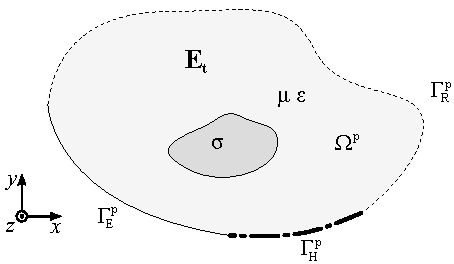
\includegraphics[width=4.5cm]{FEMproblemEigen} 
%\caption{Finite element domain for the waveport eigenvalue problem.}
\label{fig:FEMproblemEigen}
\end{figure}
\begin{equation*}
\mathbf{E} = [\mathbf{E}_{t}(x,y) + \hat{\mathbf{z}} \ E_{z}(x,y)] \ \text{e}^{-\gamma z} \quad \text{on } \Omega^p
\end{equation*}
Transverse and longitudinal basis functions $$\mathbf{v} = \hat{\mathbf{n}}\times\mathbf{w} \in \mathcal{H}(\mathrm{curl}, \Omega^p, \Gamma_E), \quad \phi \in \mathcal{H}^1(\Omega^p, \Gamma_E)$$ are introduced to expand the electric field such that
$$\mathbf{E}_{t} = \sum_{j=1}^{N_t} x_{t,j} \mathbf{v}_j, \quad E_{z} = \sum_{j=1}^{N_z} x_{z,j} \phi_j$$
}

\frame{
\frametitle{Preprocessing : Transverse-longitudinal field formulation for waveports}
Galerkin projections on
\begin{equation*}
\nabla \times \frac{1}{\mu_r} \nabla \times \mathbf{E} - {k}_0^2 {\epsilon}_r \mathbf{E} = 0
\end{equation*}
with  $\epsilon_r \leftarrow \epsilon_r + {\sigma}/{j\omega_0\epsilon_0}$
$$\Downarrow$$
$$\mat{A}\vect{x} = \lambda \mat{B}\vect{x}$$
An efficient Lanczos-based Krylov subspace solver (ARPACK) is used to compute eigenvalues $\lambda = \gamma^2$ and related eigenvectors. Coefficients $x_t$ are then orthonormalized and mapped to the original problem, in order to expand the transverse mode distributions $\mathbf{E}_t^k$.
}

\frame{
\frametitle{Preprocessing : Total field scattering problem -- weak form}
\begin{multline*}
%\label{eq:FEMformScatt}
\int_\Omega \nabla \times \mathbf{w}_i^* \cdot \frac{1}{\mu_r} \nabla \times \mathbf{E} \ d\Omega + j k_0 \zeta_0 \int_\Omega \mathbf{w}_i^* \cdot \sigma \mathbf{E} \ d\Omega \ + \\
\hspace{-1cm} j k_0 \zeta_0 \int_{\mathrm{\Gamma}_R} \hat{\mathbf{n}} \times \mathbf{w}_i^* \cdot \frac{1}{Z_s} \hat{\mathbf{n}} \times \mathbf{E} \ d\mathrm{\Gamma} \ - 
 k_0^2 \int_\Omega \mathbf{w}_i^* \cdot \epsilon_r \mathbf{E} \ d\Omega \ = \\
 j k_0 \zeta_0 \int_{\Gamma_{R}} \hat{\mathbf{n}} \times \mathbf{w}_i^* \cdot \left( \frac{1}{Z_s} \hat{\mathbf{n}} \times \mathbf{E}^{inc} - \mathbf{H}^{inc} \right) \ d\Gamma, \quad \forall \mathbf{w}_i \in \mathcal{W}_E
\end{multline*}
$$\Downarrow$$
$$\mat{A} \ \vect{x}   =  \vect{b}$$
$\mat{A} \in \mathbb{C}^{N \times N}$, $\vect{x}$ and $\vect{b} \in \mathbb{C}^{N}$
}

\frame{
\frametitle{Assembly : Element matrices computation}
Efficient computation of higher-order finite element matrices by quadrature integration and mappings on reference element
%\footfullcite{rognes2009efficient} 

\begin{columns}
    \begin{column}{0.65\textwidth}
$$
\int_{K} f(x,y,z) \ dx dy dz = \int_{K_0} f(\xi, \eta, \zeta) \ \det\mat{J} \ d\xi d\eta d\zeta
$$
\begin{equation*}
\begin{aligned}
\phi(x,y,z) \ & \longrightarrow \ \phi(\xi, \eta, \zeta)\\
\nabla\phi(x,y,z) \ & \longrightarrow \ \mat{J}^{-1} \nabla \phi(\xi, \eta, \zeta)
\end{aligned}
\end{equation*}
$$\int_{K_0} f(\xi, \eta, \zeta) \ \det\mat{J} \ d\xi d\eta d\zeta \approx \sum_q^{N_q} f(\xi_q, \eta_q, \zeta_q) \ w_q $$
    \end{column}

    \begin{column}{0.35\textwidth}
      \centering
      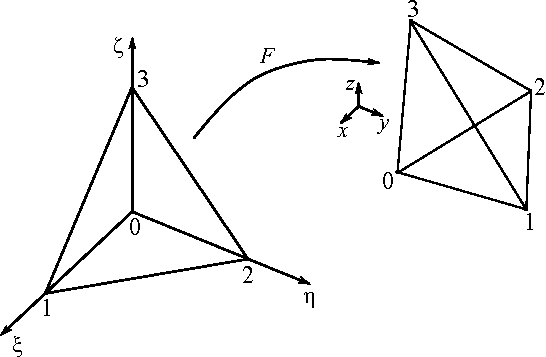
\includegraphics[width=4cm]{MappingTet}
    \end{column} 
  \end{columns} 
}

\frame{
\frametitle{Assembly : Sparse matrix assembly}
\begin{itemize}
\item Multicore enabled element matrices computation with OpenMP
\item Spase matrix storage scheme:  $O(N^2) \rightarrow O(N)$ (GMM++  library)
\item Global ordering of mesh entities such that
\begin{eqnarray*}
E \lbrace i,j\rbrace & \ \text{with} & \ i < j\\
F \lbrace i,j,k\rbrace & \ \text{with} & \ i < j < k\\
T \lbrace i,j,k,l \rbrace & \text{with} & \ i < j < k < l
\end{eqnarray*}
leads to fast global matrix unknowns mapping
$$\begin{bmatrix}
A_{1,1} & A_{1,2} & \ldots & A_{1,p}\\
A_{2,1} & A_{2,2} &  & \vdots\\ 
\vdots & & \ddots & \vdots\\
A_{p,1} & \ldots & \ldots & A_{p,p}
\end{bmatrix}$$
\item Isotropic materials lead to a symmetric system matrix allowing to approximately halve memory requirements
\end{itemize}
}

\frame{
\frametitle{Solution : direct or iterative solver}
\begin{itemize}
\item Sparse direct solver
\begin{itemize}
\item At best $O(N^2)$ memory requirements
\item Very fast and accurate solution, especially if multithreaded arithmetic is employed
\end{itemize}
\item Iterative solver
\begin{itemize}
\item At best $O(N)$ memory requirements
\item Krylov subspace solvers guarantee the convergence in at most N iterations
\item Solution times strongly depend on matrix conditioning -- need for good preconditioners
\end{itemize}
\end{itemize}

FES employs the public domain MUMPS package (single and double precision complex values) with multhreaded BLAS as direct solver, and a C++  implementation of  the Krylov subspace solver GMRES
}

\frame{
\frametitle{Postprocessing}
The system solution allows to recover several parameters that describe the electromagnetic behavior of the modeled problem. Some of these are
\begin{itemize}
\item Scattering parameters at the ports
\item Radiation parameters such as the far fields, directivity and gain for antenna problems, radar cross sections for scattering problems
\item The electromagnetic fields visualization in $\Omega$
\end{itemize}
}

\frame{
\frametitle{Postprocessing : Scattering parameters}
\begin{itemize}
\item Dominant mode continuity
$$S_{mk} = \frac{1}{2} \int_{\Gamma_{WG}^m}  \mathbf{E}^* \cdot \frac{1}{Z_m} \mathbf{E}_t^{m \ inc} \ d\Gamma - \delta_{mk}, \qquad m = 1, \ldots,  N^M$$
\item Transfinite element method
$$S_{mk} = a_m^r - \delta_{mk}, \qquad m = 1, \ldots,  N^M$$
\end{itemize}
}

\frame{
\frametitle{Postprocessing : Radiation parameters}
\begin{itemize}
\item Radiated field (Stratton-Chu formulas in Kottler's form) \small
\begin{eqnarray*}
{\mathbf{E}}(\hat{\mathbf{r}}) &=  &j\zeta_0k_0 \frac{\mathrm{e}^{-jkr}}{4\pi r} \int_{\Gamma_R}  \mathrm{e}^{jk \hat{\mathbf{r}} \cdot \mathbf{r}'} \left [ \left ( \hat{\mathbf{n}}\times\mathbf{H}(\mathbf{r}') \cdot \hat{\mathbf{r}} \right ) \hat{\mathbf{r}} - \hat{\mathbf{n}}\times\mathbf{H}(\mathbf{r}') \right ] \ d\Gamma \ - \nonumber \\ 
& &  \quad jk_0 \frac{\mathrm{e}^{-jkr}}{4\pi r} \int_{\Gamma_R} \mathrm{e}^{jk \hat{\mathbf{r}} \cdot \mathbf{r}'} \ \mathbf{E}(\mathbf{r}')\times\hat{\mathbf{n}}  \times \hat{\mathbf{r}}  \ d\Gamma
\end{eqnarray*}
\item \normalsize Directivity and gain
$$
D(\hat{\mathbf{r}}) =   \lim_{r\to\infty} 2 \pi r^2 \frac{|\mathbf{E}(\hat{\mathbf{r}})|^2}{\zeta_0 P_\mathrm{rad}}, \quad
G(\hat{\mathbf{r}}) =   \lim_{r\to\infty} 2 \pi r^2 \frac{|\mathbf{E}(\hat{\mathbf{r}})|^2}{\zeta_0 P_\mathrm{in}}
$$
$$P_\mathrm{rad} = \int_{\Gamma_R} \mathbf{E}^*\times\mathbf{H} \cdot \hat{\mathbf{n}} \ d\Gamma, \quad P_\mathrm{in} = - \int_{\Gamma_{WG}} \mathbf{E}^*\times\mathbf{H} \cdot \hat{\mathbf{n}} \ d\Gamma$$
\item Radar cross section
\begin{equation*}
\label{eq:RCS}
RCS (\hat{\mathbf{r}}) = \lim_{r\to\infty} 4 \pi r^2 \frac{|\mathbf{E}(\hat{\mathbf{r}})|^2}{|\mathbf{E}^{inc}|^2}
\end{equation*}
\end{itemize}
}


\frame{
\frametitle{Postprocessing : Fields visualization}
\begin{itemize}
\item Fields can be recovered everywhere in $\Omega$ remembering that
$$\mathbf{E}_E(\mathbf{r}) := \sum_{j=1}^{N} x_j \mathbf{w}_j(\mathbf{r})$$
$$\mathbf{H}_E(\mathbf{r}) := \sum_{j=1}^{N} x_j \frac{\nabla \times \mathbf{w}_j(\mathbf{r})}{-j k_0\zeta_0\mu_r(\mathbf{r})}$$
\\[.5cm]
\begin{equation*}
\mathbf{w}_j(\mathbf{r}) = \left\lbrace
\begin{array}{cc}
\mathbf{w}_j(\mathbf{r}), & \mathbf{r} \in K\\
0, & \mathbf{r} \not\in K\\
\end{array}
\right.
\end{equation*}
$K$ is any element of $\mathcal{M}_h(\Omega)$
\end{itemize}
FES relies on Paraview (VTK format) for fields and radiation solids visualization
}

\subsection{Validation examples}
\frame{
\frametitle{Example : Millimeter-wave E-plane bandpass filter}
\begin{figure}[ht!]
\centering
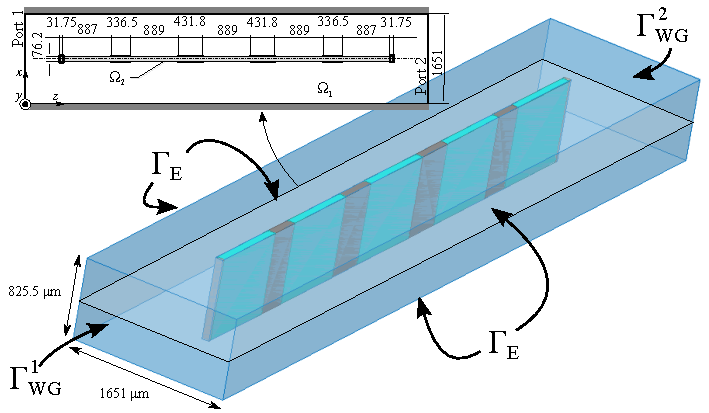
\includegraphics[width=8cm]{Bui1984}
%\caption{Sketch for the millimeter-wave waveguide filter analyzed and its cross section (H-plane). Measures are given in $\mu m$. }
\label{fig:Bui1984}
\end{figure}
\centering
$\epsilon_r = 2.1 \in \Omega_2$\\
Mesh of 9~686 tetrahedra, $p=2 \rightarrow 57~524$ unknowns

}

\frame{
\frametitle{Example : Millimeter-wave E-plane bandpass filter}
\begin{figure}[ht!]
\centering
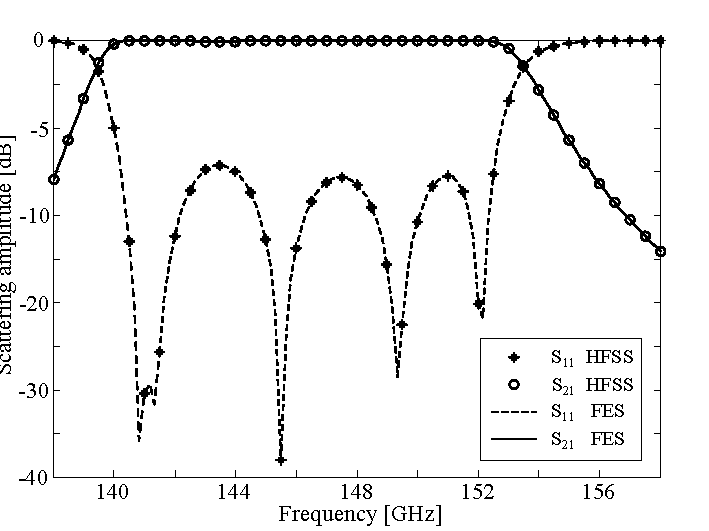
\includegraphics[width=7cm]{Bilat3Dresponse}
\label{fig:Bilat3Dresponse}
\end{figure}
\begin{table}[h!]
\begin{center}
\begin{tabular}{|c|c|c|c|}
\hline 
Dominant (s) & Dominant (d) & Transfinite (s) & Transfinite (d) \\ 
\hline
\hline
$   1.5351 \ 10^{-6}$ & $1.3643 \ 10^{-6}$ & $5.6383 \ 10^{-7}$ & $1.6853 \ 10^{-12}$ \\ 
\hline 
\end{tabular}
\end{center}
%\caption{Comparison between the average Euclidean errors for both waveport continuity formulations (only dominant $\mathrm{TE}_{10}$ mode retained), varying the solver precision (s=single, d=double).}
\label{tab:Bilatprecision}
\end{table}

}

\frame{
\frametitle{Example : Millimeter-wave E-plane bandpass filter}
Electric field at 150~GHz\\[1cm]
\centering
HFSS \qquad \qquad \qquad \qquad  FES \\
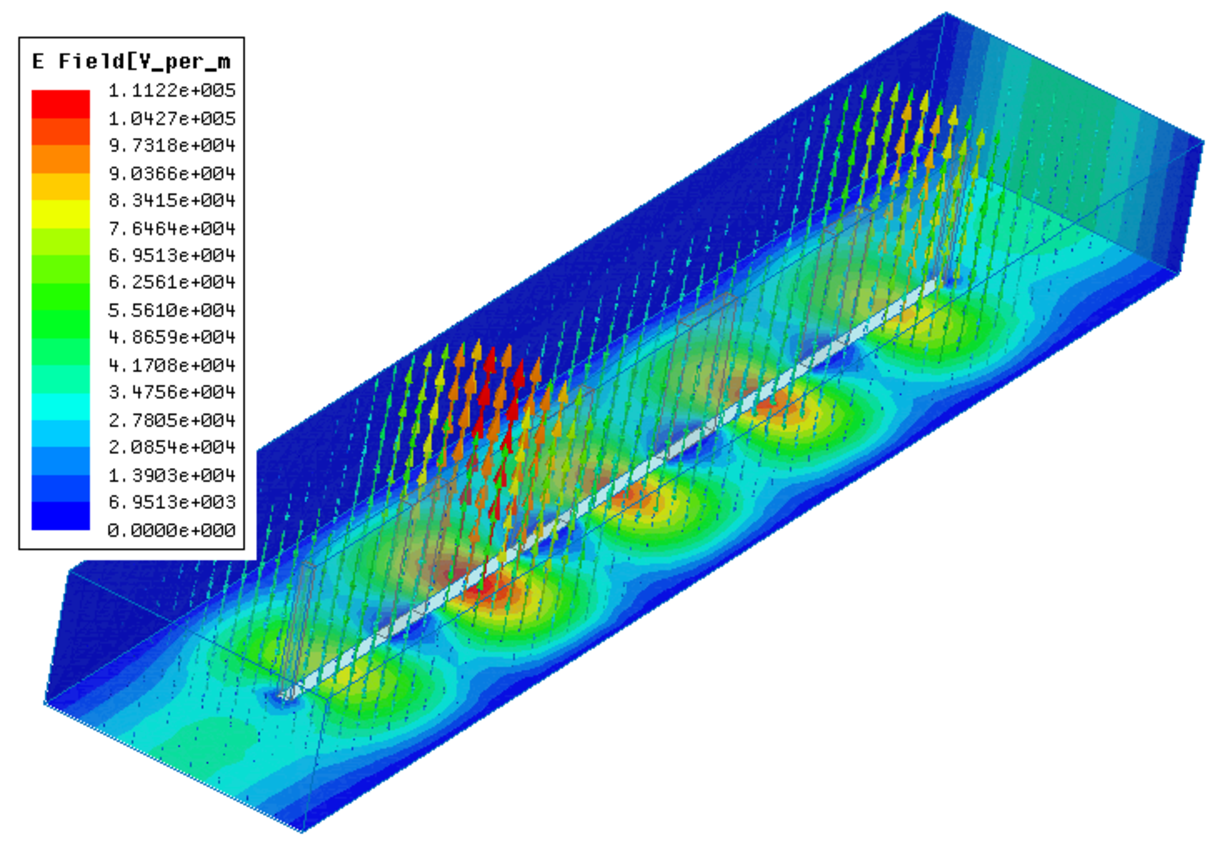
\includegraphics[width=.45\textwidth]{Bilat3DHFSS} \ 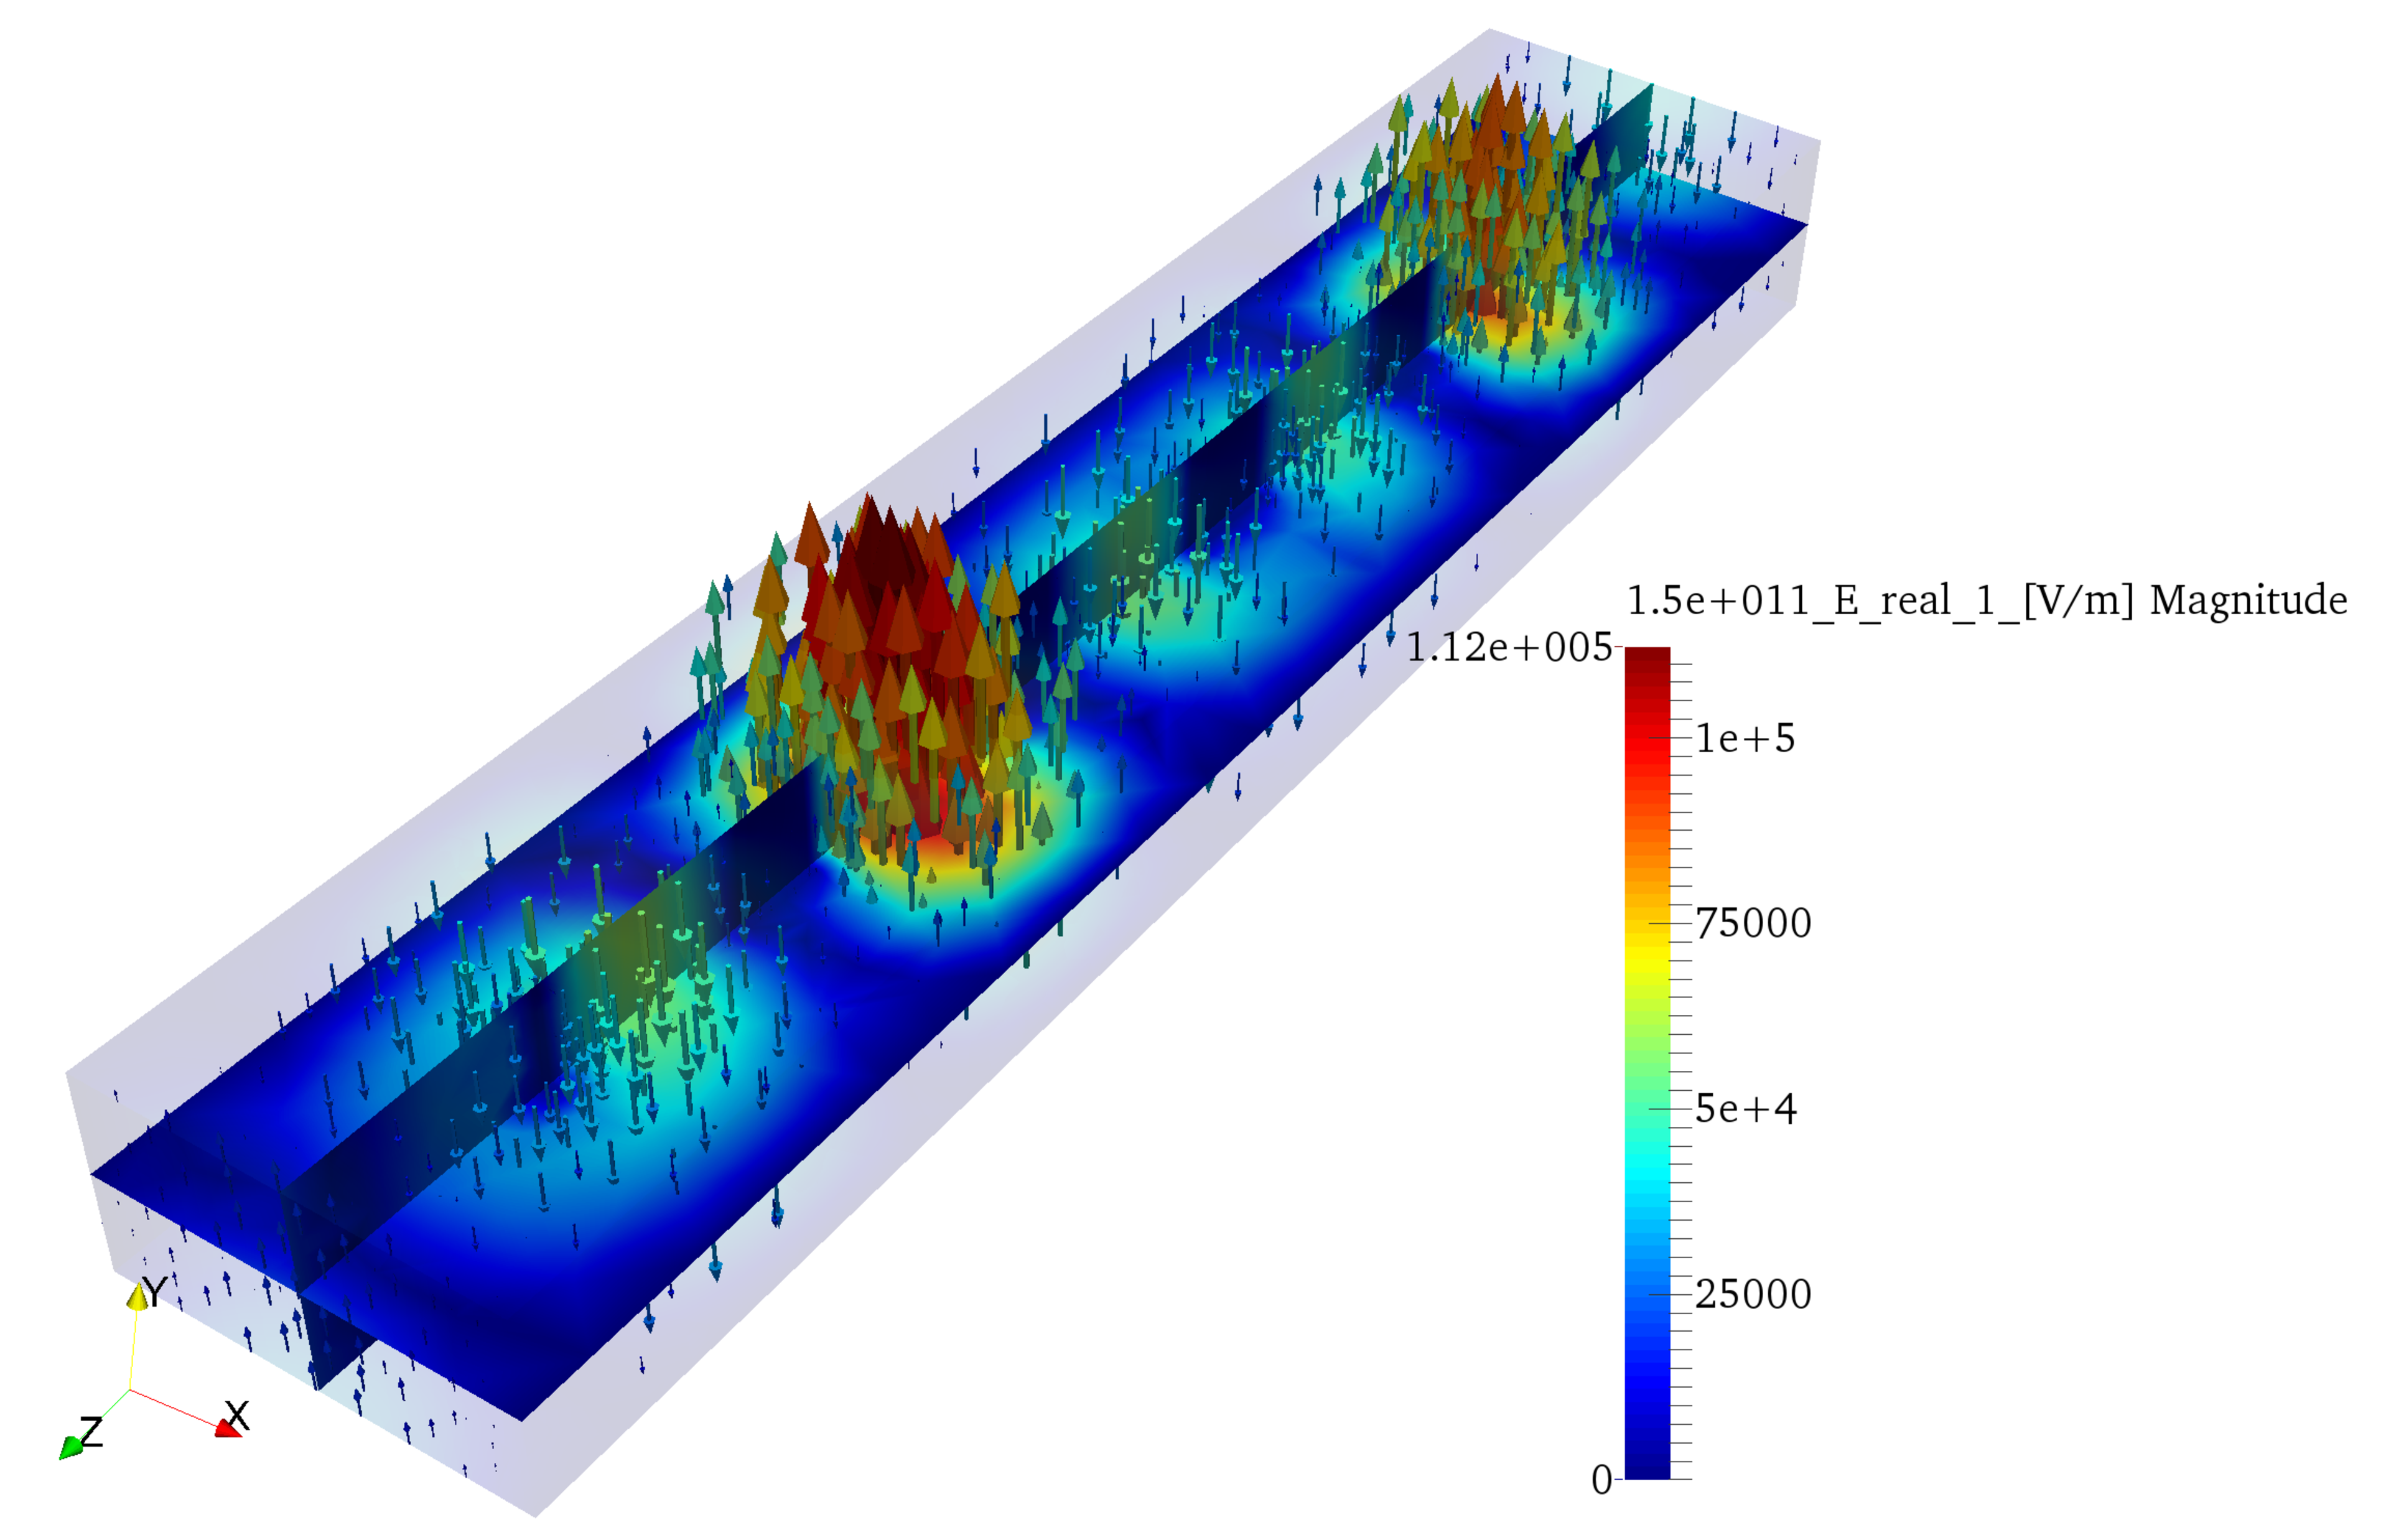
\includegraphics[width=.45\textwidth]{Bilat3D}
}

\frame{
\frametitle{Example : 22 GHz corrugated circular horn antenna}
\begin{figure}[ht!]
\centering
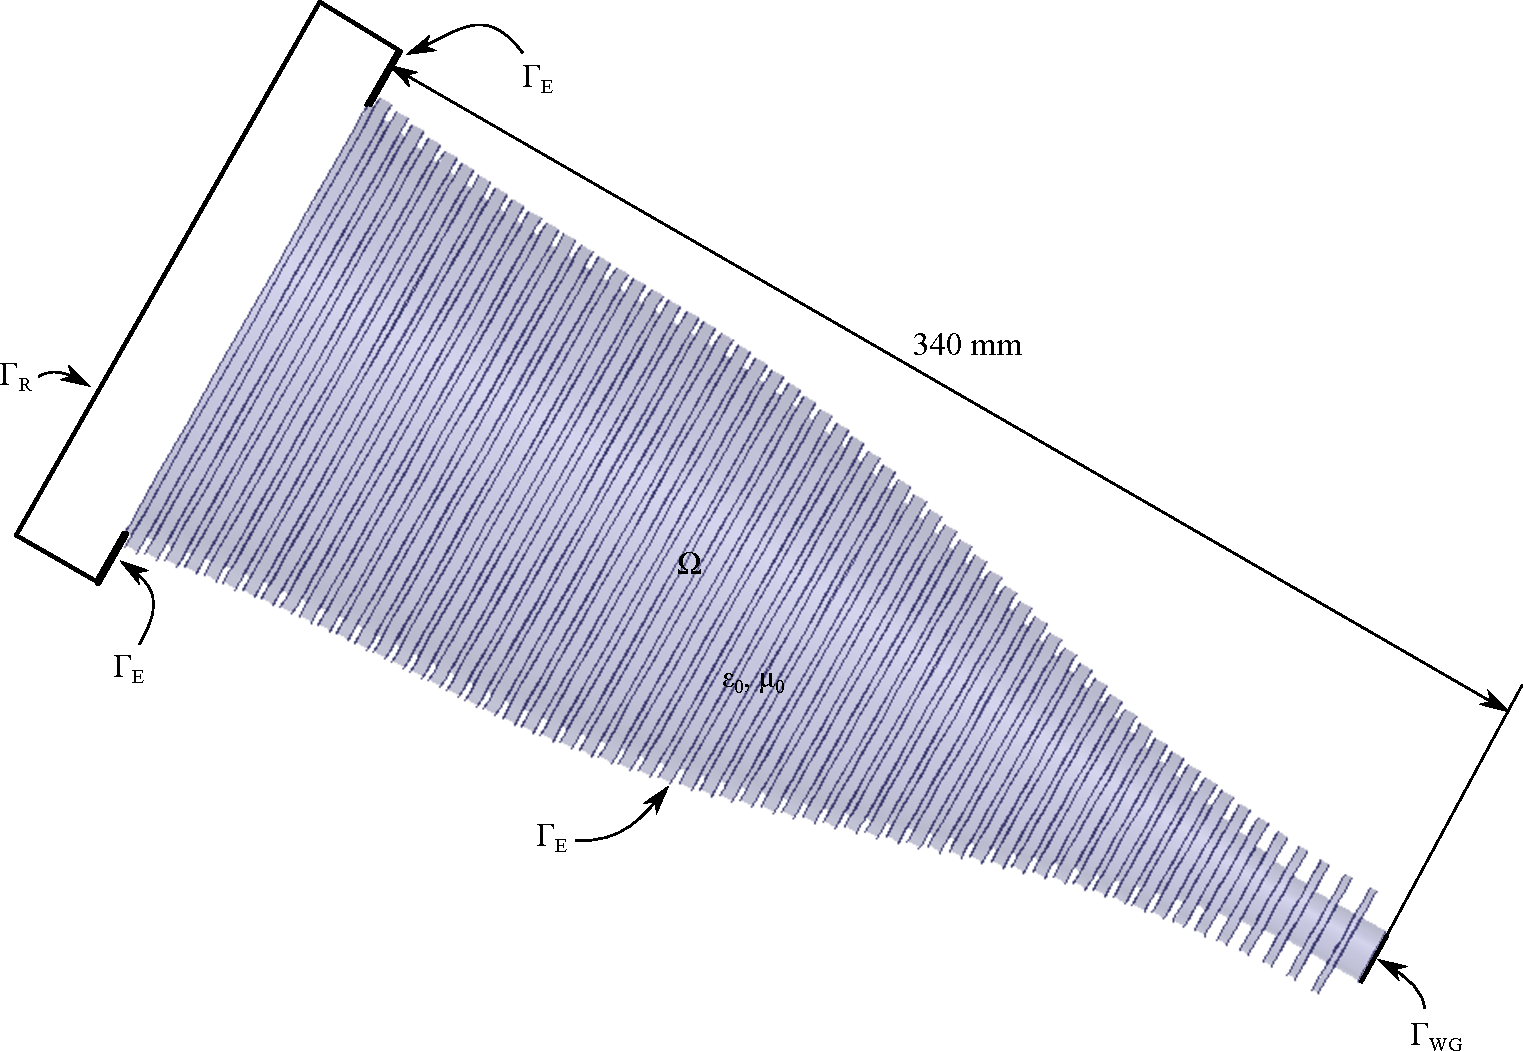
\includegraphics[width=8cm]{CircHornSketch}
\label{fig:CircHornSketch}
\end{figure}
\centering
\quotes{Osservatorio Astrofisico di Arcetri}\\ 60 corrugations to achieve linear polarization\\
36~331 tetrahedra, $p=3 \rightarrow  602~594$ unknowns
}

\frame{
\frametitle{Example : 22 GHz corrugated circular horn antenna}
Degenerate $\text{TE}_{11}$ modes feeding the antenna (in quadrature) computed with the ARPACK solver\\
\centering
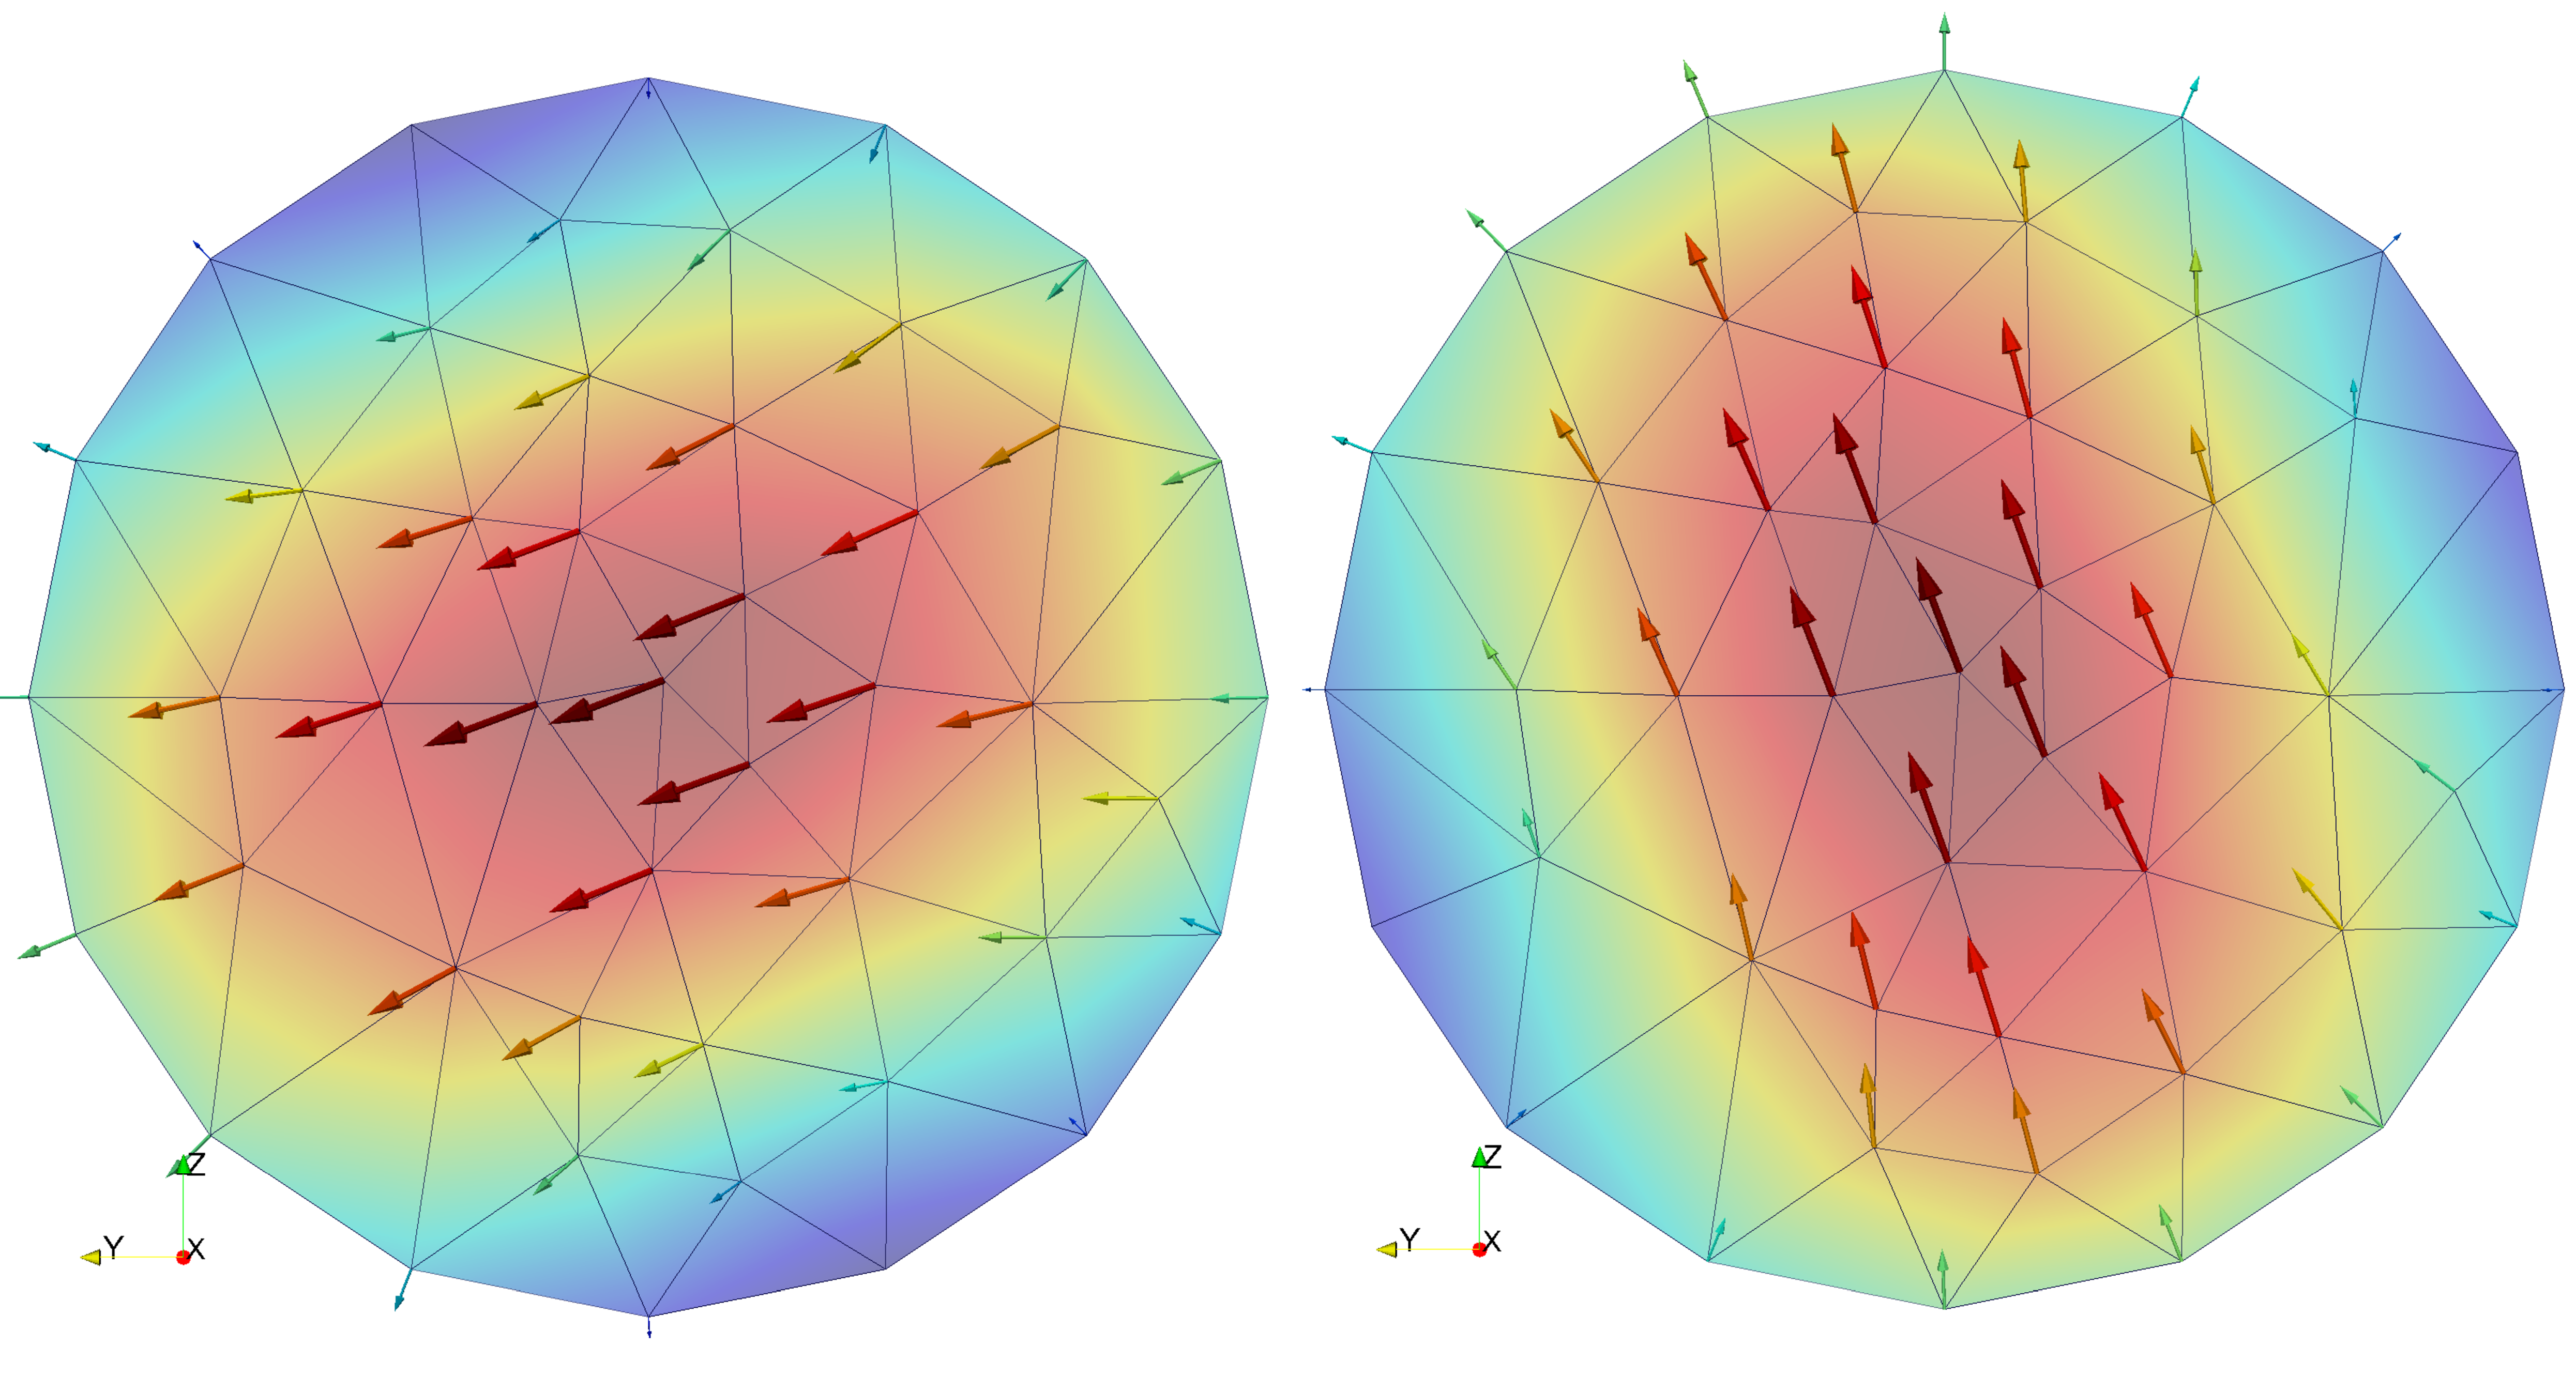
\includegraphics[width=5cm]{Modes}
\begin{table}[h!]
\begin{center}
\begin{tabular}{|c|c|c|c|}
\hline 
Solver & FES (s) & FES (d) & HFSS (m) \\ 
\hline
\hline
Time & 123 s & 170 s & 146 s\\ \hline
Memory & 3158 MB & 6159 MB & 3.7 GB\\ \hline
Relative error & $7 \ 10^{-5}$ & $6.5 \ 10^{-5}$ & -- \\
\hline 
\end{tabular}
\end{center}
\end{table}
}

\frame{
\frametitle{Example : 22 GHz corrugated circular horn antenna}
\centering
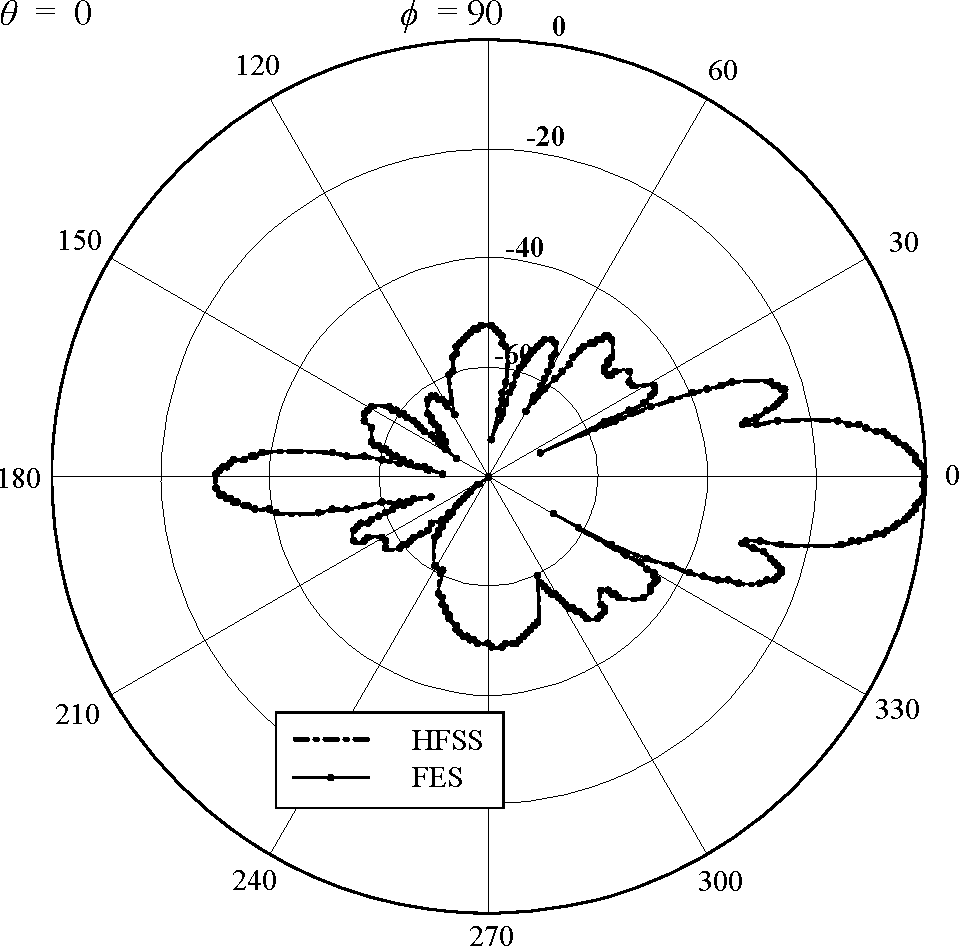
\includegraphics[width=5cm]{Polar2} \  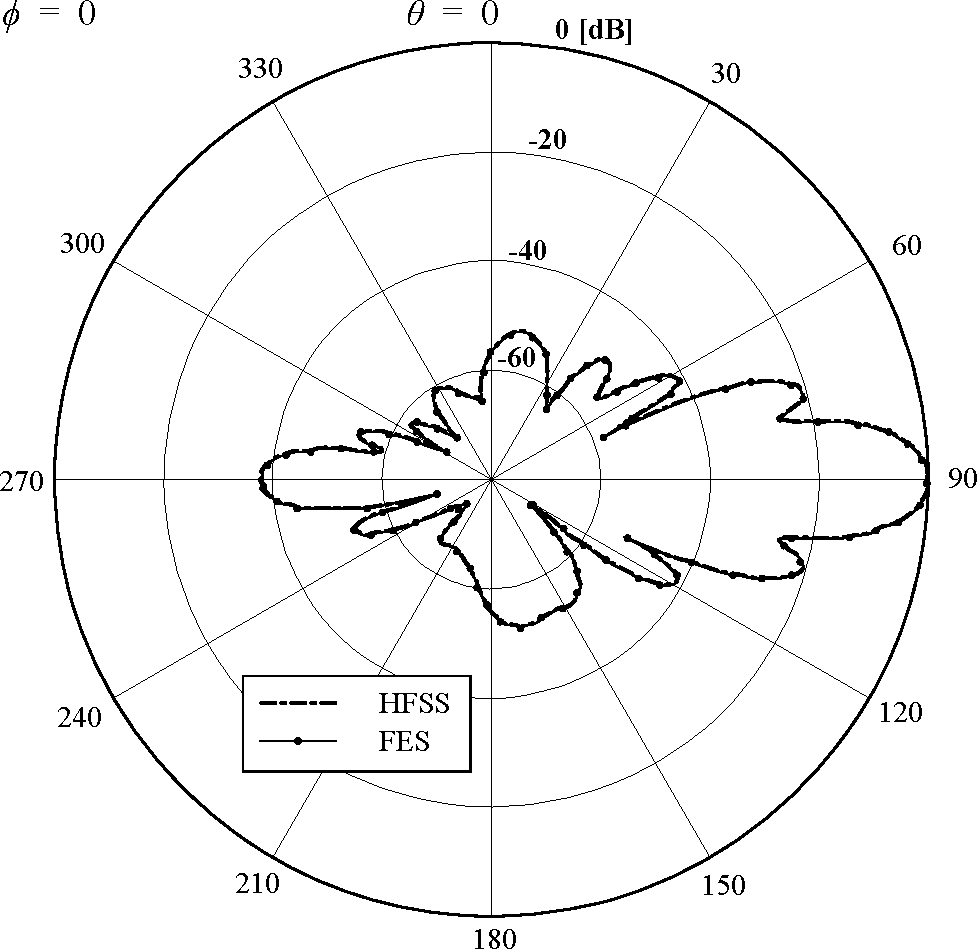
\includegraphics[width=5cm]{Polar1}\\
Normalized gain patterns on the \textit{XY} (left) and the \textit{XZ} (right) planes
}

\frame{
\frametitle{Example : Perfect electric sphere scattering}
\centering
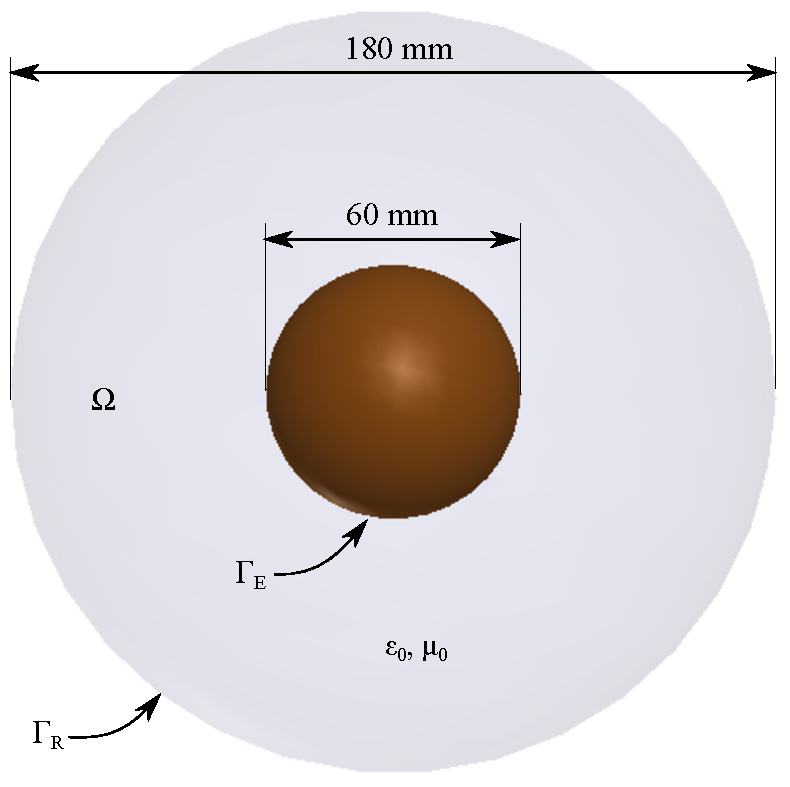
\includegraphics[width=5cm]{Sphere}\\
$$\mathbf{E}^{inc} = | \mathbf{E}^{inc}| \exp{-jk_0 \hat{\mathbf{z}} \cdot \mathbf{r} } \ \hat{\mathbf{x}}, \quad \mathbf{H}^{inc} = \frac{1}{\zeta_0} \mathbf{E}^{inc} \times \hat{\mathbf{z}} =  \frac{1}{\zeta_0}| \mathbf{E}^{inc}| \exp{-jk_0 \hat{\mathbf{z}} \cdot \mathbf{r} } \ \hat{\mathbf{y}}$$
Mesh of 73~252 tetrahedra, $p=1 \rightarrow 89~946$ unknowns
}

\frame{
\frametitle{Example : Perfect electric sphere scattering}
\centering
HFSS \qquad \qquad \qquad \qquad  FES \\
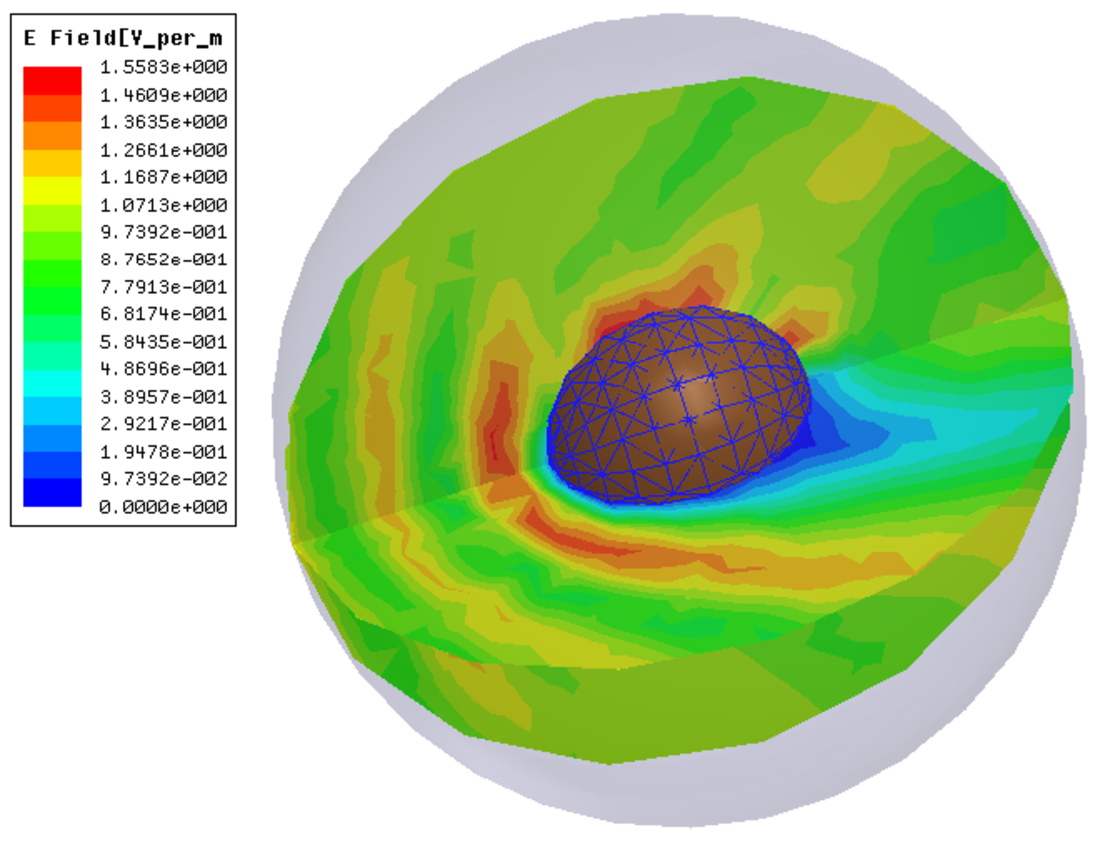
\includegraphics[width=4.5cm]{SphereHFSS} \ \  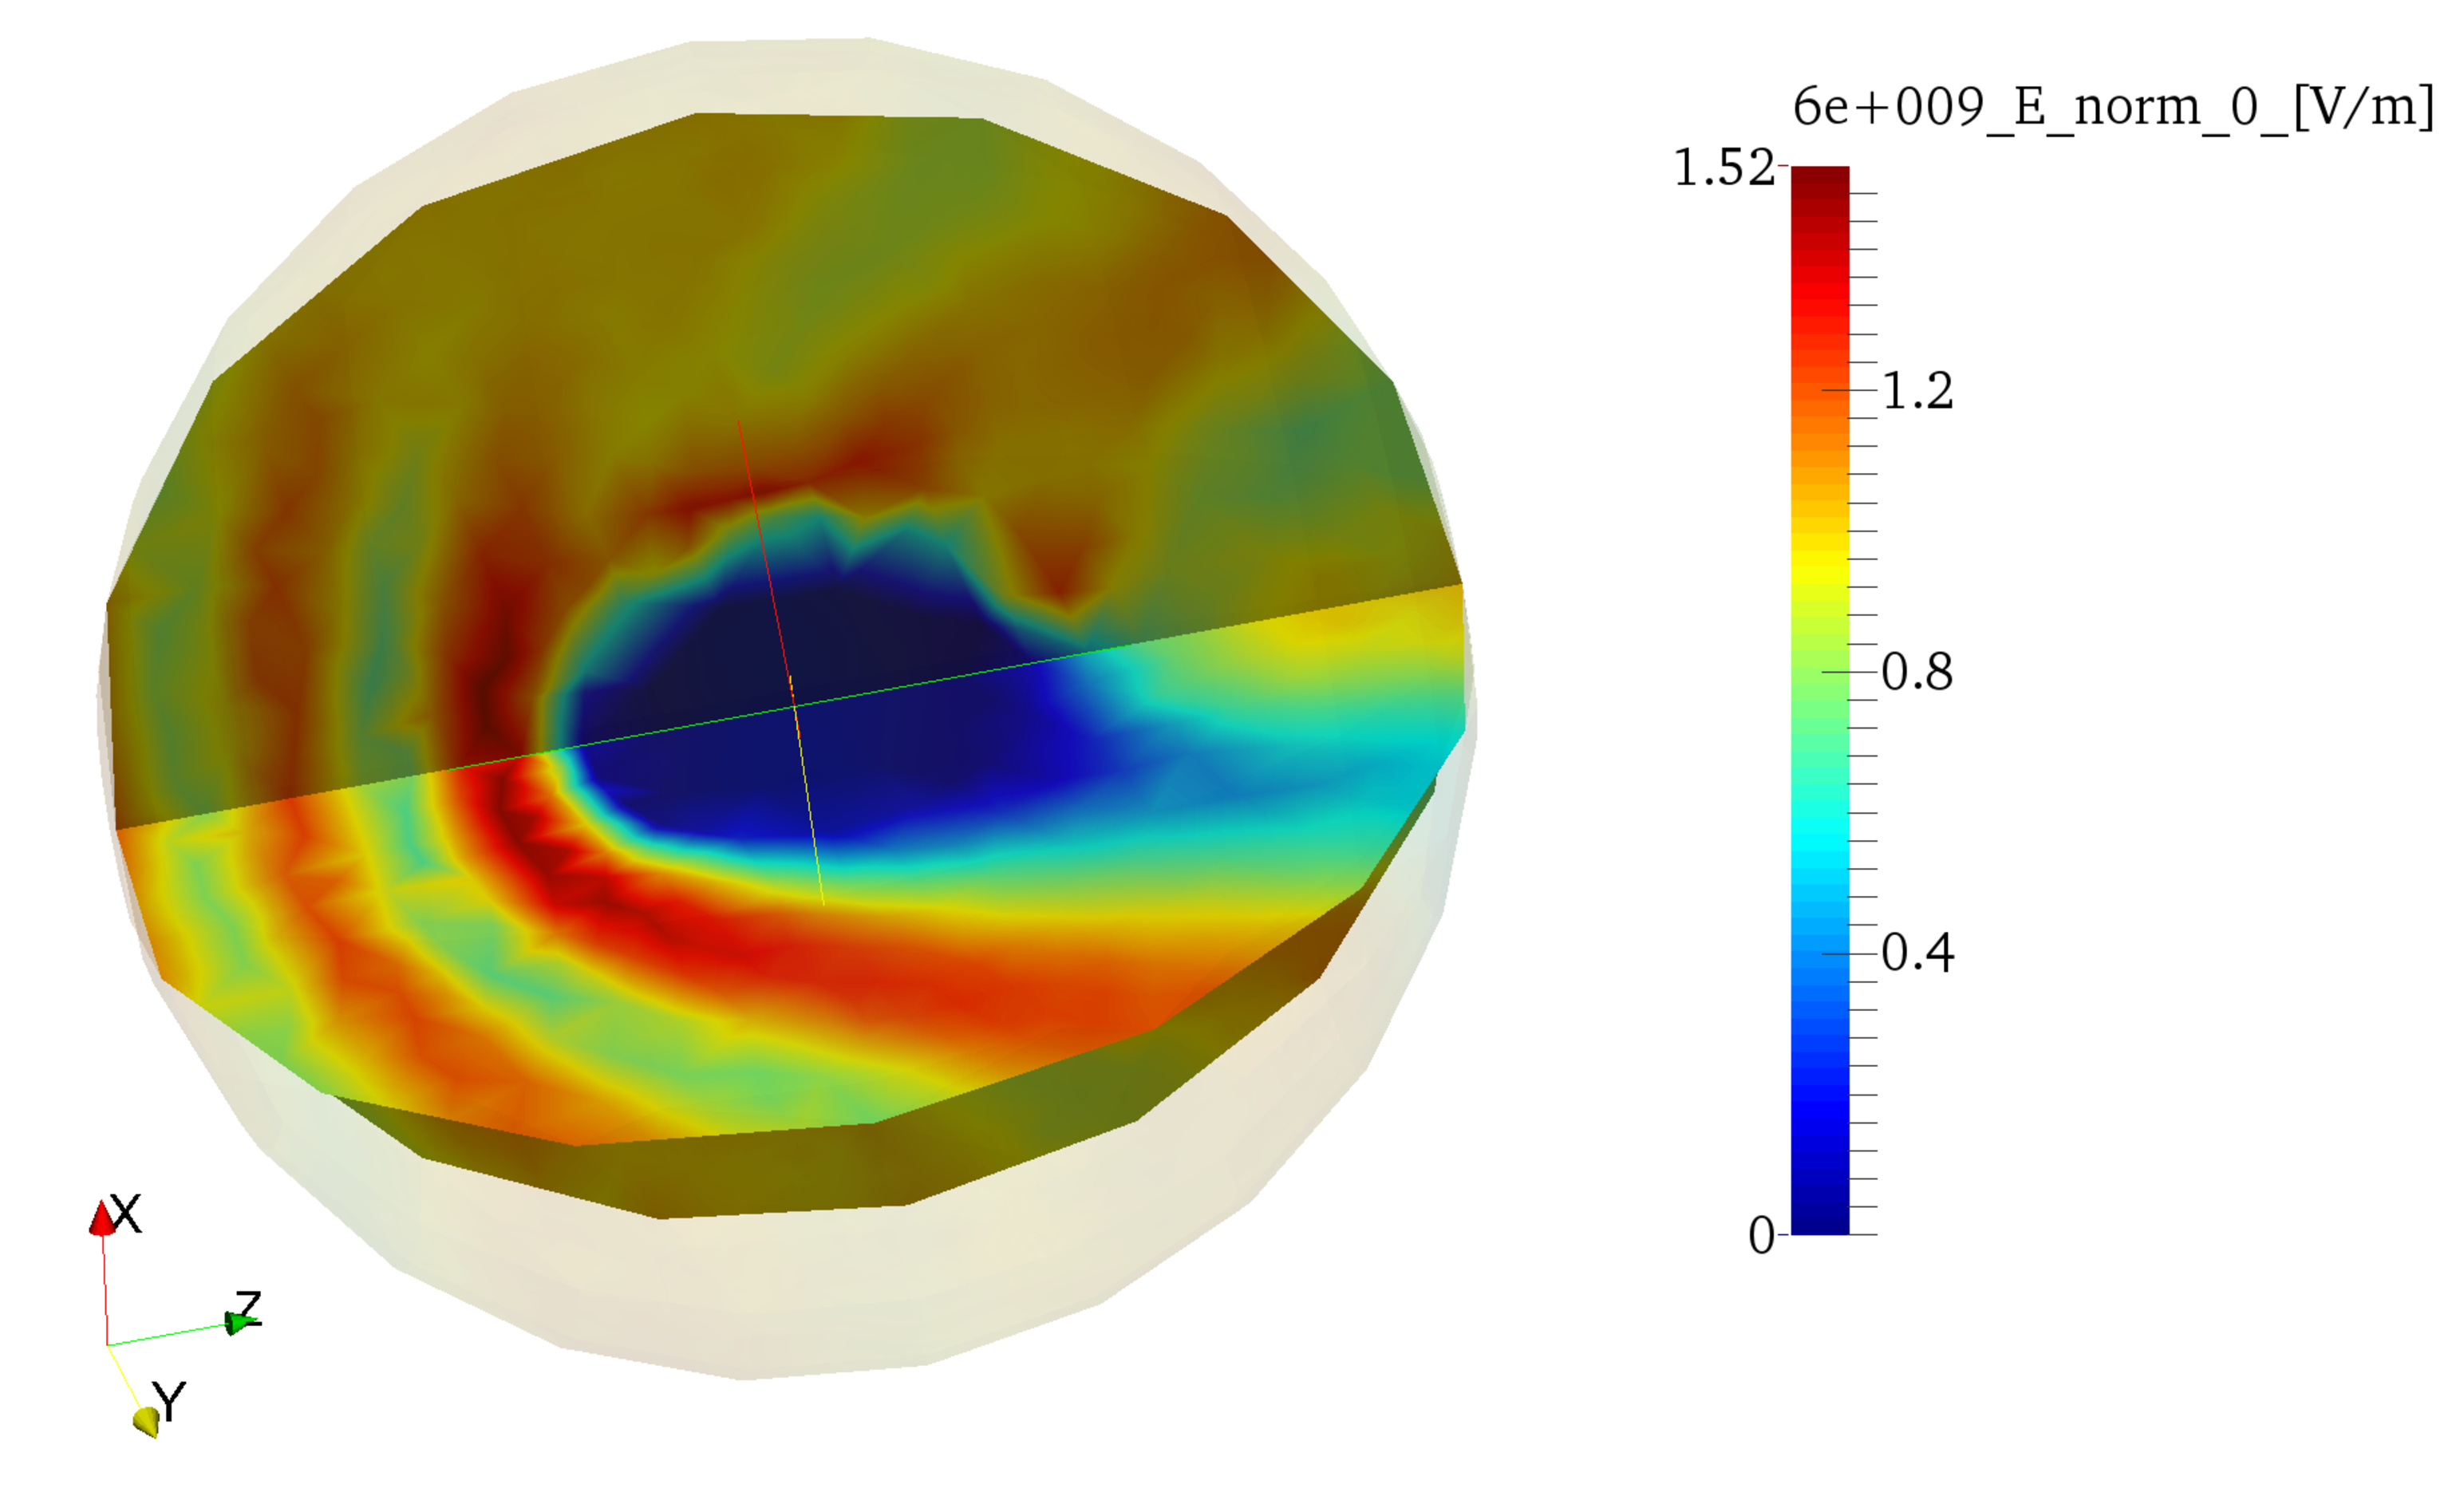
\includegraphics[width=6cm]{SphereField}\\
 $ |\mathbf{E}|_{\max} \approx 1.52~\frac{\text{V}}{\text{m}}$

}

\frame{
\frametitle{Example : Perfect electric sphere scattering}

\centering
HFSS \qquad \qquad \qquad \qquad  FES \\
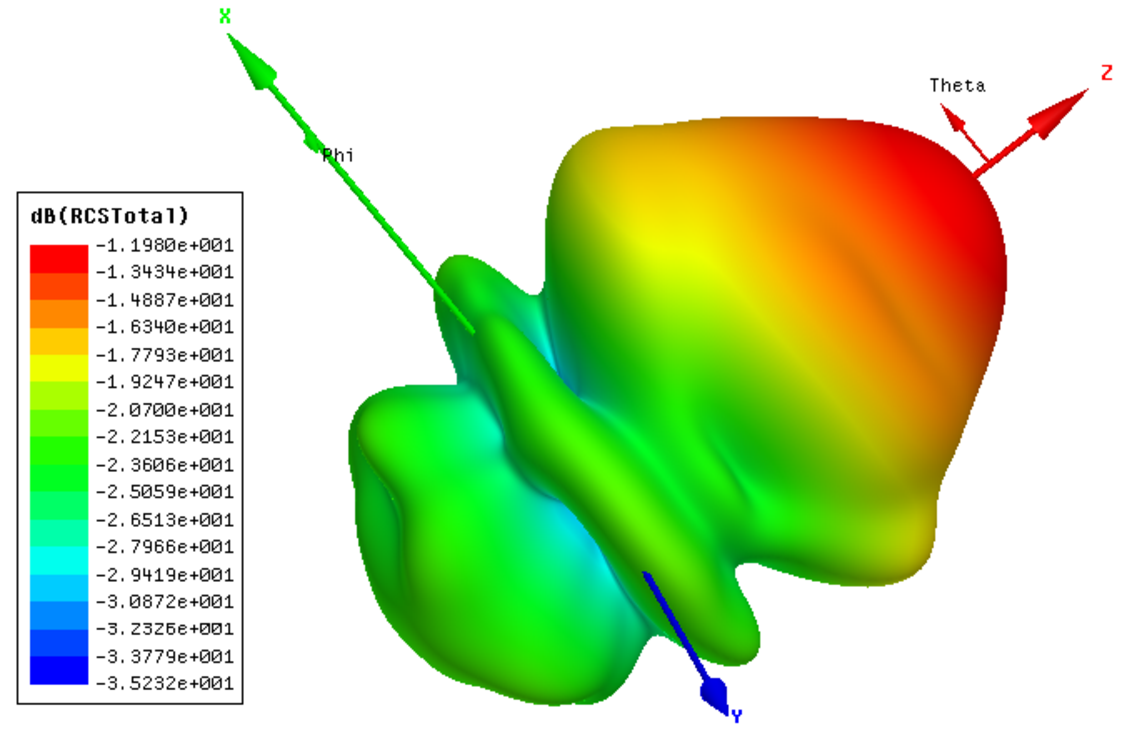
\includegraphics[width=5.7cm]{SphereRCSHFSS} \ \  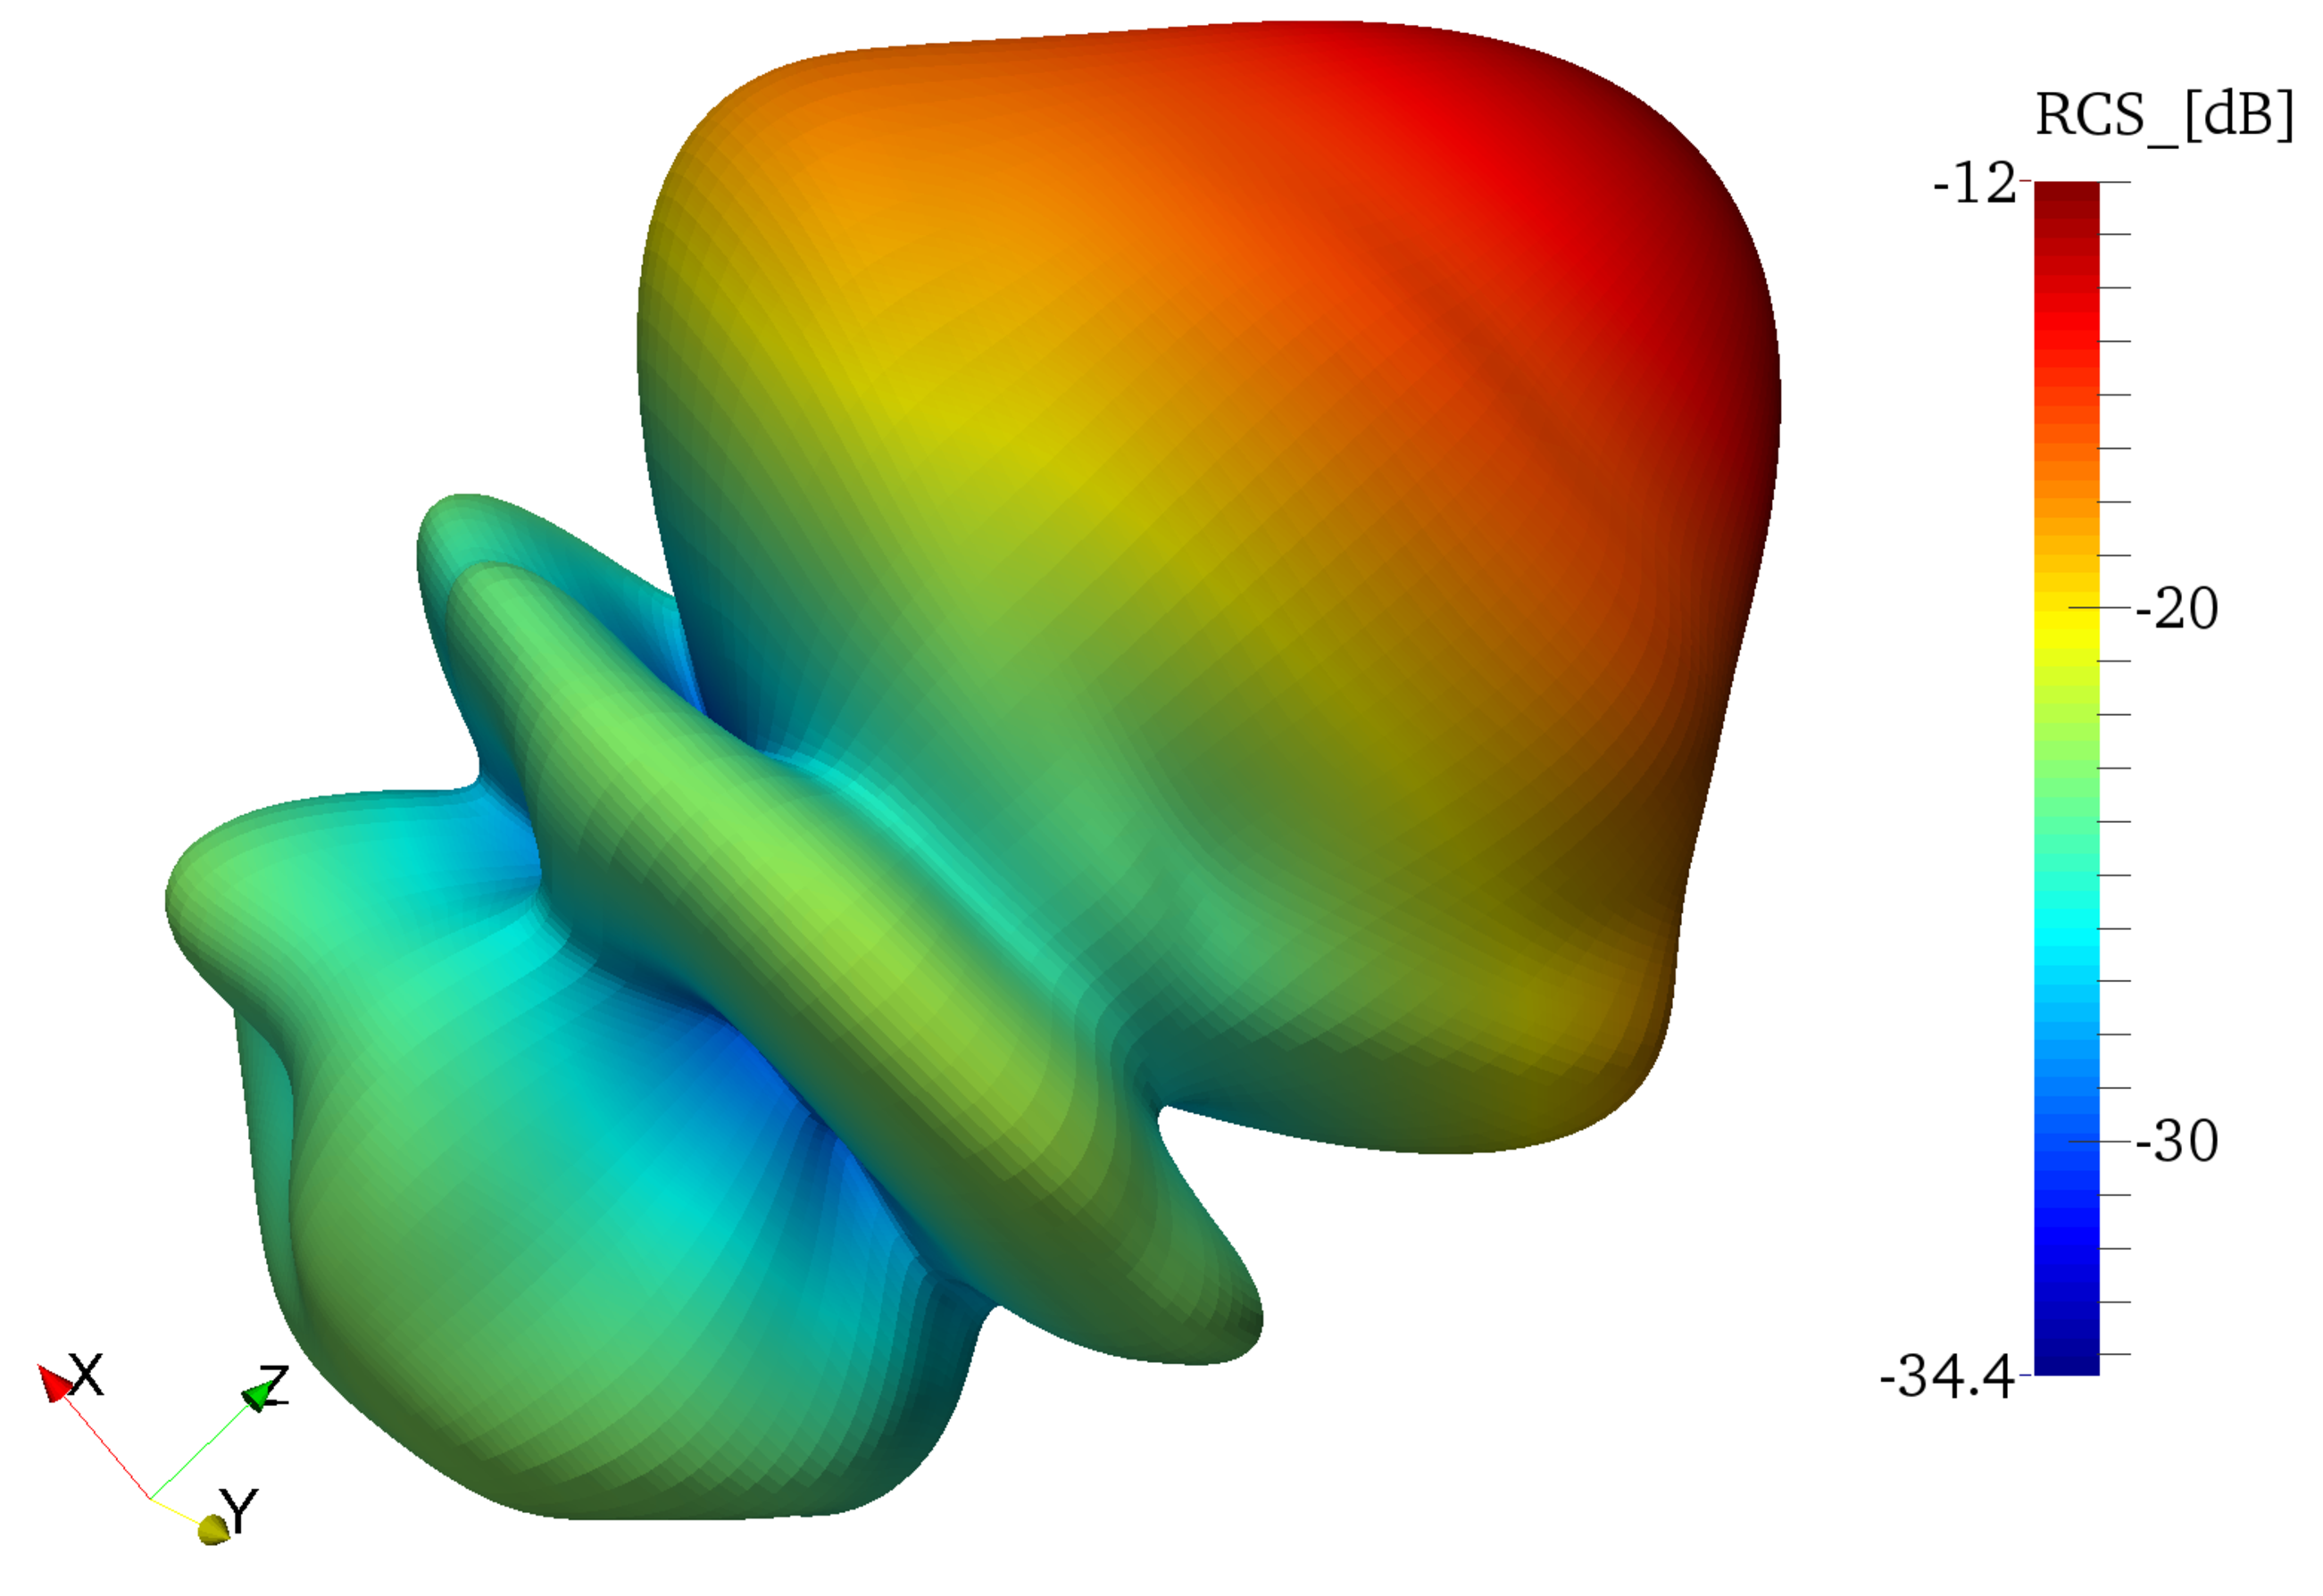
\includegraphics[width=4.7cm]{SphereRCS}\\
$ RCS_{\max} \approx -12~\text{dB}$\\
\begin{table}[h!]
\begin{center}
\begin{tabular}{|c|c|c|c|}
\hline 
Solver & FES (s) & FES (d) & HFSS (m) \\ 
\hline
\hline
Relative error & $4.49 \ 10^{-4}$ & $9.21 \ 10^{-5}$ & -- \\
\hline 
\end{tabular}
\end{center}
\end{table}

}

\frame{
\frametitle{Example : Perfect electric sphere scattering}
FES (Paraview) vector visualization features\\
\centering
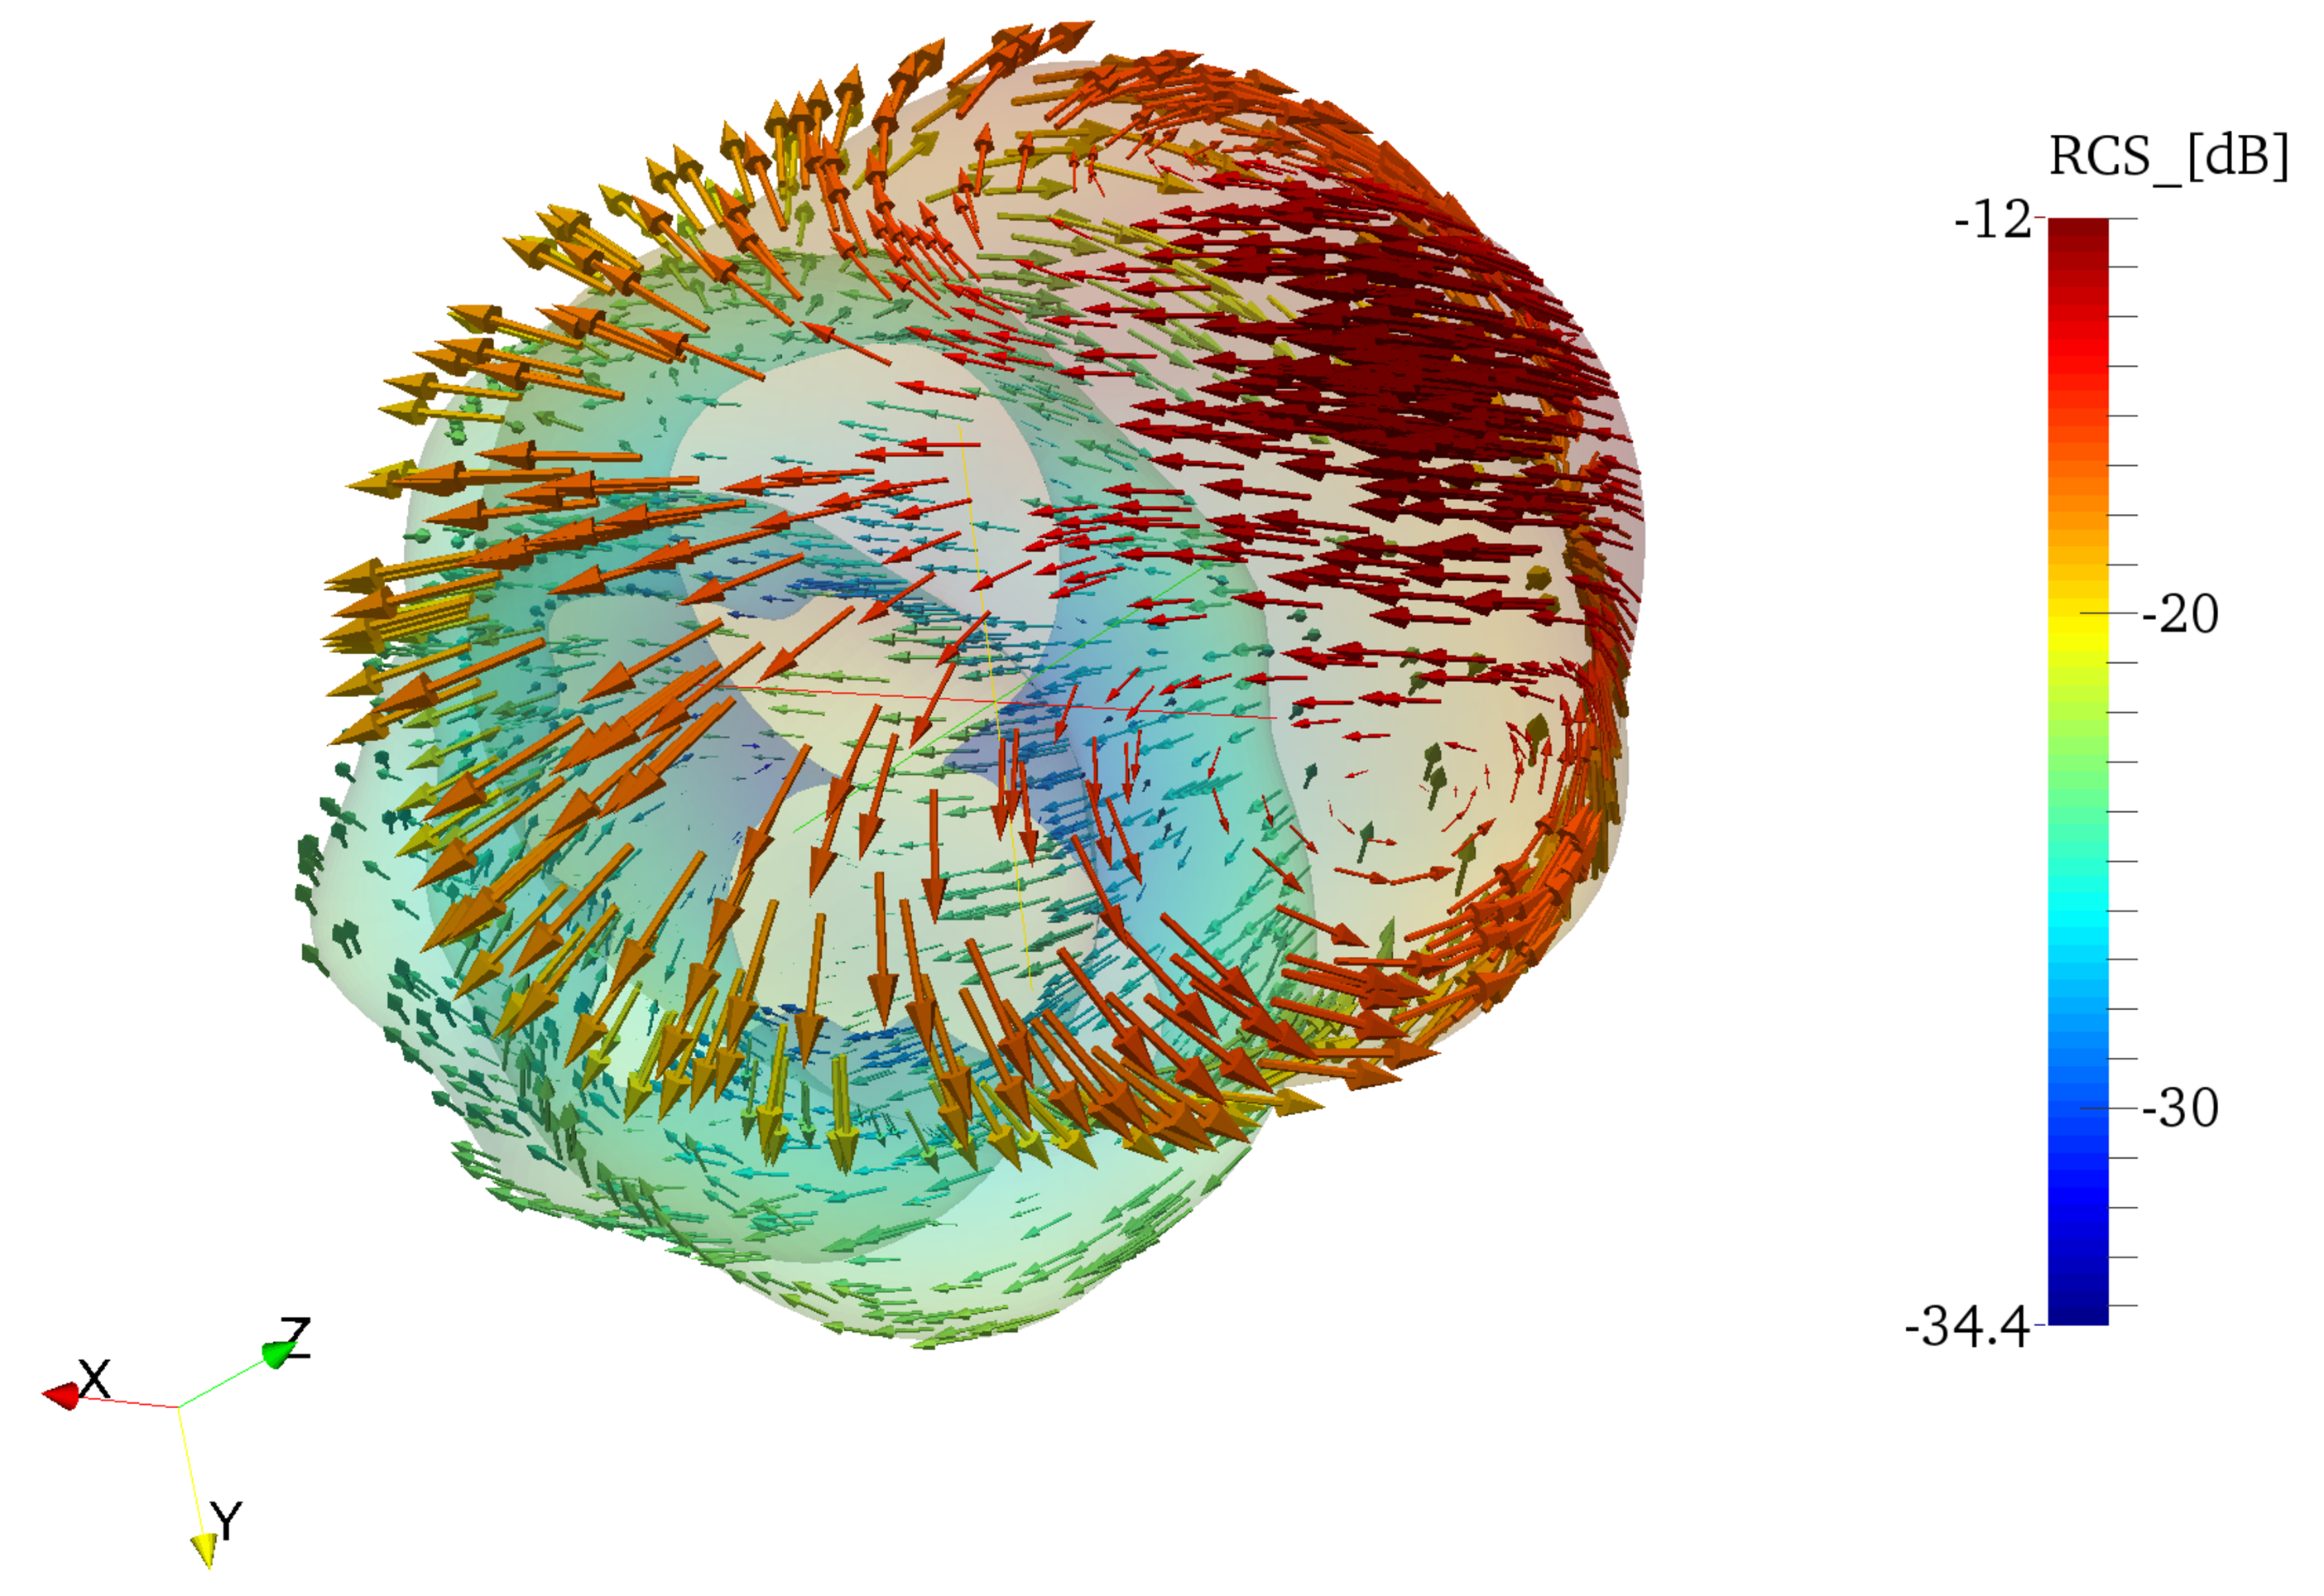
\includegraphics[width=8cm]{SpherePol}

}

\graphicspath{{img/ch2/}}

\section{Domain decomposition methods for large problems}
\subsection{Introduction}

\frame{
\frametitle{\textit{Divide et impera} concept for large problems}
\centering
Overalapping and non-overlapping\\[.2cm]
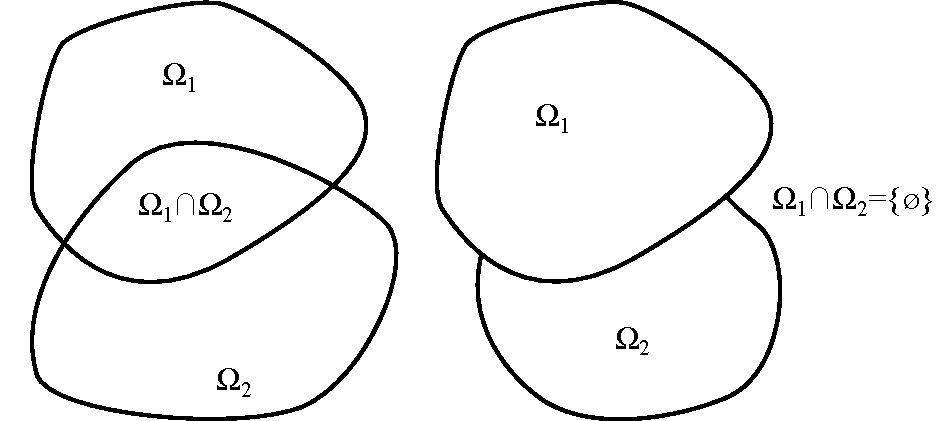
\includegraphics[width=8cm]{DDnonoverlaping}
\begin{block}{}
Investigation of two non-overapping domain decomposition methods
\begin{itemize}
\item  a Schur Complement based method 
\item  a Finite Element Tearing and Interconnecting Dual-Primal (FETI-DP) based method 
\end{itemize}
\end{block}
}

\subsection{Schur Complement based domain decomposition}
\frame{
\frametitle{Schur Complement based method }
\begin{center}
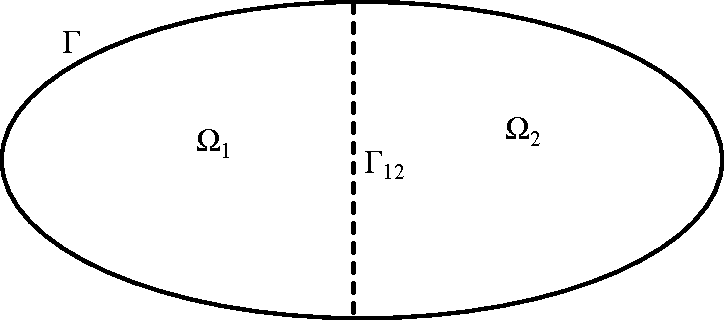
\includegraphics[width=6cm]{DDSchur2}\\
\end{center}
Assuming isotropic materials
\begin{equation}
\label{eq:DDSchurSym}
\begin{bmatrix}
A_{\Gamma\Gamma} & A_{\Gamma1} & A_{\Gamma2}\\
A_{\Gamma1}^T & A_{11} & \\
A_{\Gamma2}^T &  & A_{22}
\end{bmatrix}
\begin{bmatrix}
x_{\Gamma}\\
x_{1}\\
x_{2}
\end{bmatrix}
=
\begin{bmatrix}
B_{\Gamma}\\
\phantom{B}\\
\phantom{B}
\end{bmatrix}
\end{equation}
Subscript $\Gamma$ refers to shape functions with related mesh entity on $\Gamma \equiv \Gamma_E \cup \Gamma_H \cup \Gamma_R \cup \Gamma_{WG} \cup \Gamma_{12}$

}

\frame{
\frametitle{Schur Complement based method : Assembly and solution procedure }
\begin{itemize}
\item Assemble the Schur complement matrix $\mat{S} = \mat{A_{\Gamma\Gamma}} - \sum_{j=1}^2 \mat{A_{\Gamma j}} \mat{A_{jj}}^{-1} \mat{A_{\Gamma j}}^T$ and the relative right-hand side $\mat{G} = \mat{B_{\Gamma}}$,
\item Solve the Schur complement system $\mat{x_\Gamma} = \mat{S}^{-1} \mat{G}$,
\item Recover for the internal unknowns $\mat{x_j} = \mat{A_{jj}}^{-1} (-\mat{A_{\Gamma j}}^T \mat{x_\Gamma})$.
\end{itemize}
}

\frame{
\frametitle{Test case of 24 cm WR90 waveguide segment }
\centering
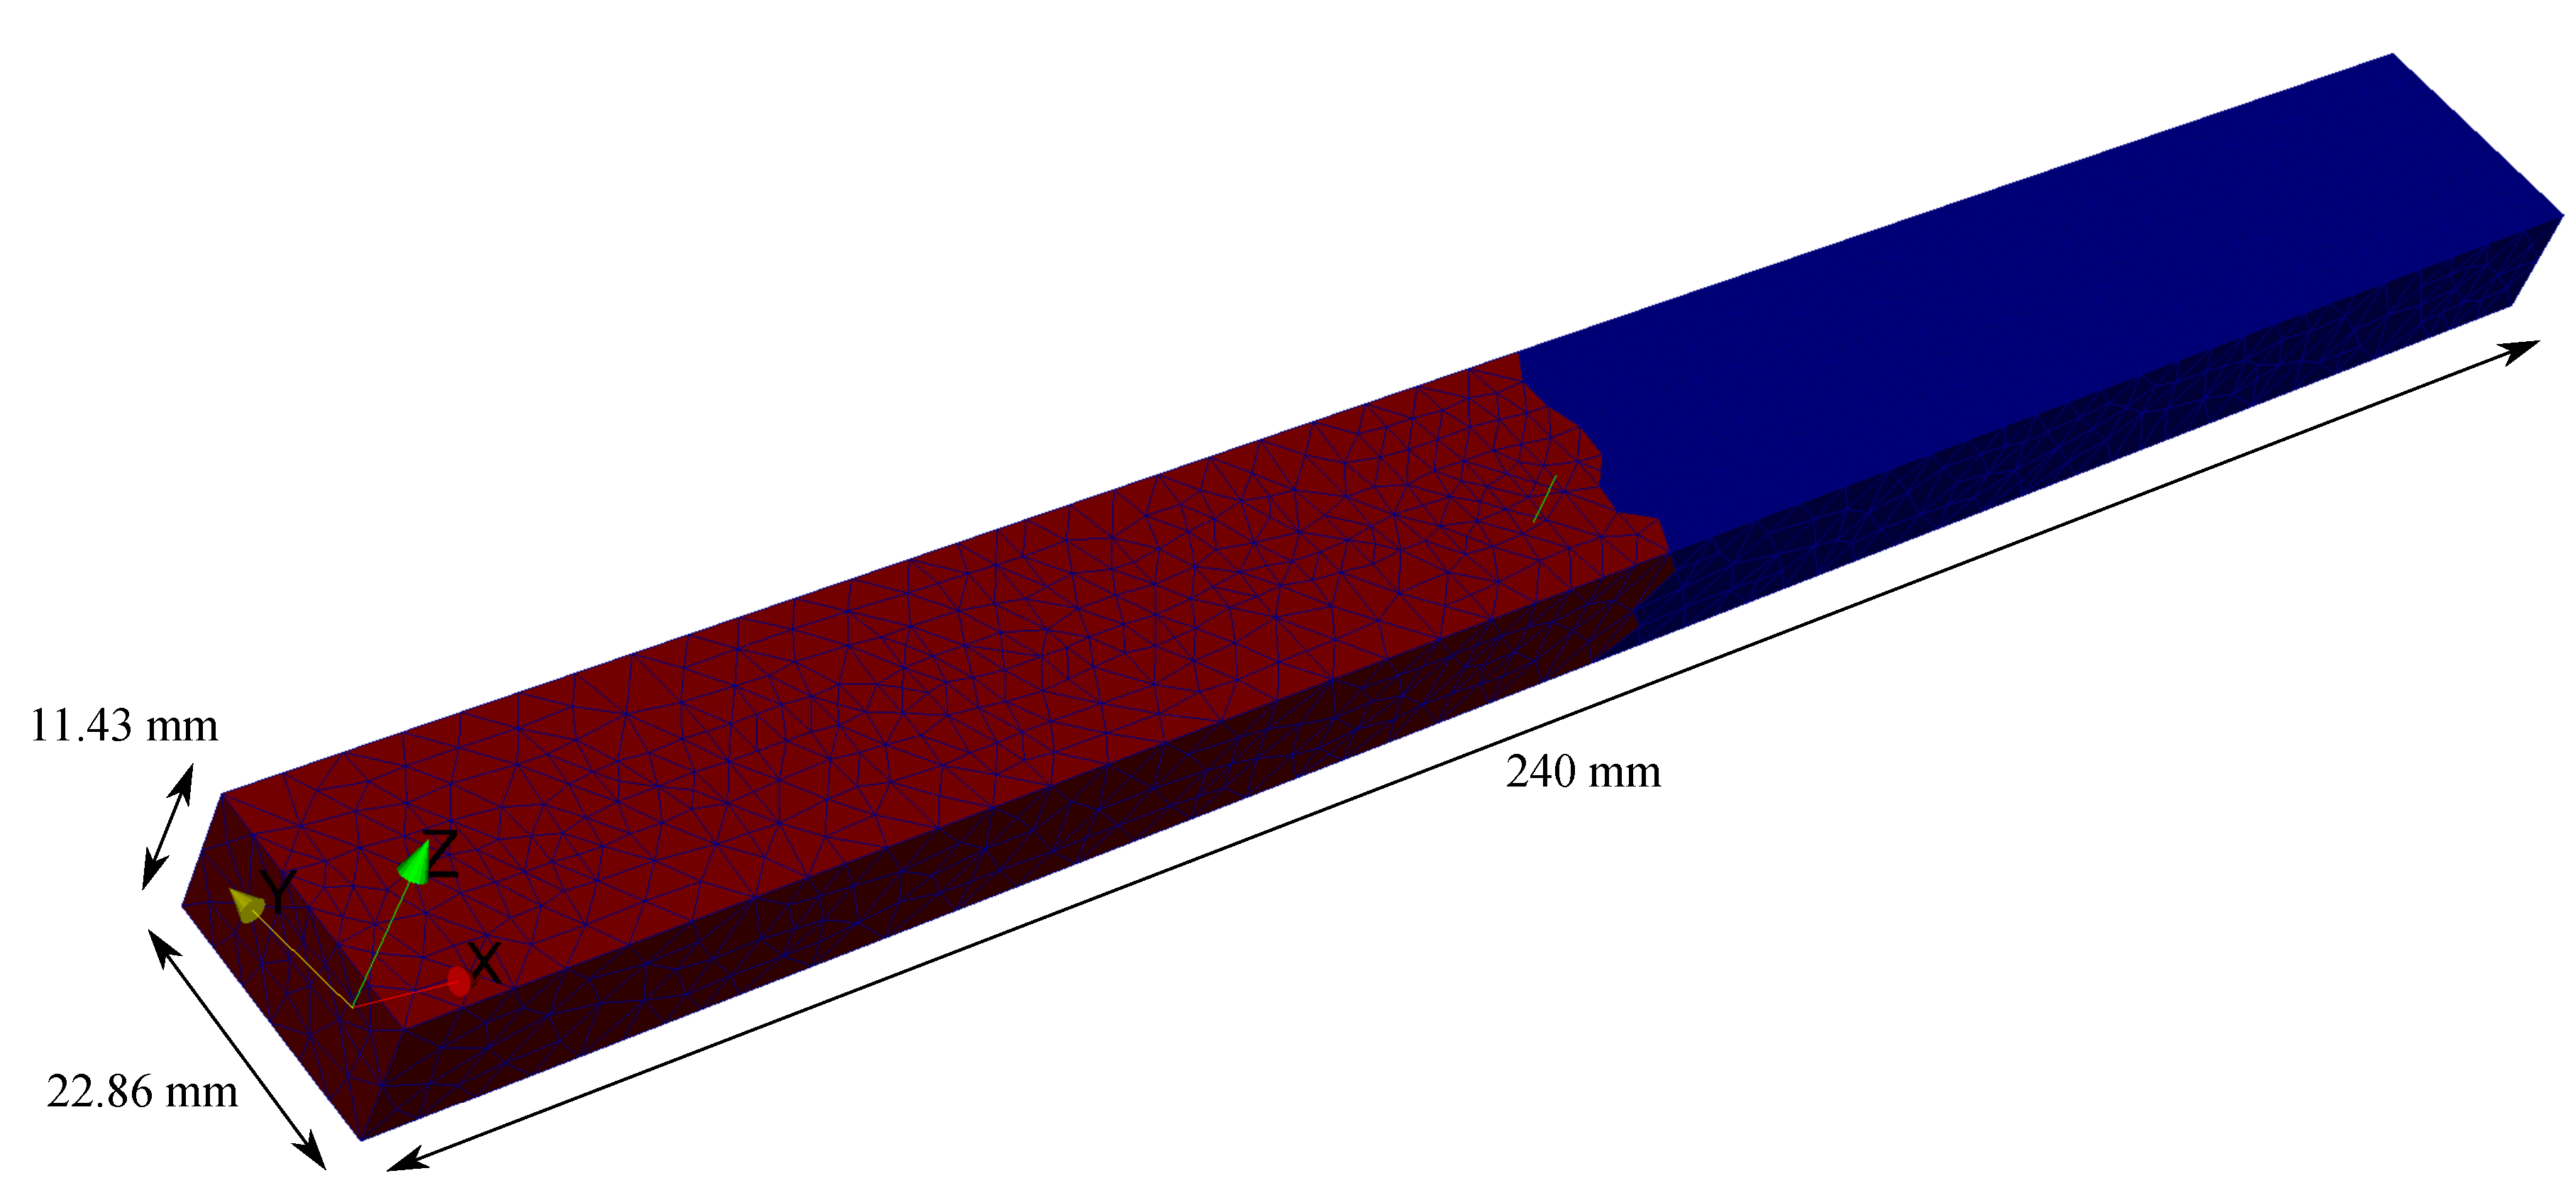
\includegraphics[width=8cm]{WR90Part}\\
20~602 tetrahedra partitioned with METIS public domain package in 10~489 and 10~113 tetrahedra\\
$p=1$
}

\frame{
\frametitle{Test case of 24 cm WR90 waveguide segment }
Direct Schur solution times and memory requirements\\[0.2cm]
\centering
\begin{table}[ht!]
\begin{center}
\begin{tabular}{|c|c|c|}
\hline 
Step & Time & Memory \\ 
\hline
\hline 
$\mat{A_{\Gamma 1}} \mat{A_{11}}^{-1} \mat{A_{\Gamma 1}}^T$ (8557) & 5.2~s & 10~MB\\ \hline 
$\mat{A_{\Gamma 2}} \mat{A_{22}}^{-1} \mat{A_{\Gamma 2}}^T$ (8082) & 4.8~s & 9.5~MB\\ \hline 
$\mat{x_\Gamma} = \mat{S}^{-1} \mat{G}$ (155) & 0.002~s & $<$ 1~MB\\ \hline 
$\mat{x_1} = \mat{A_{11}}^{-1} (-\mat{A_{\Gamma 1}}^T \mat{x_\Gamma})$ & 0.15~s &  2~MB\\ \hline 
$\mat{x_2} = \mat{A_{22}}^{-1} (-\mat{A_{\Gamma 2}}^T \mat{x_\Gamma})$ & 0.14~s &  2~MB\\ \hline 
\end{tabular}
\end{center}
%\caption
\label{tab:SchurSol}
\end{table}
}


\frame{
\frametitle{Test case of 24 cm WR90 waveguide segment }
Frequency response of the WR-90 waveguide segment computed with the Schur complement algorithm\\[0.2cm]
\centering
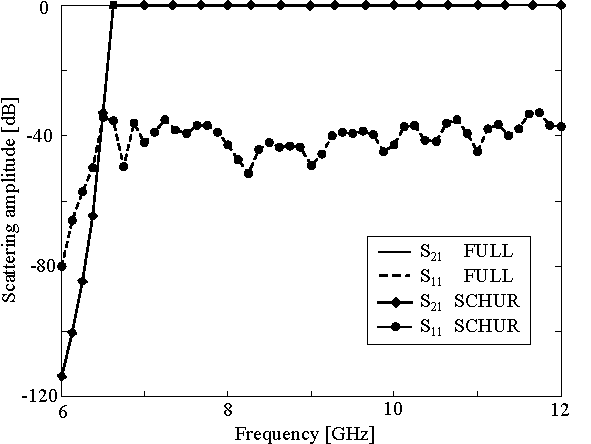
\includegraphics[width=7cm]{WRfreqSchur}
}

\frame{
\frametitle{Test case of 24 cm WR90 waveguide segment }
Upper triangular part of the Schur complement based domain decomposition system matrix\\[0.2cm]
\centering
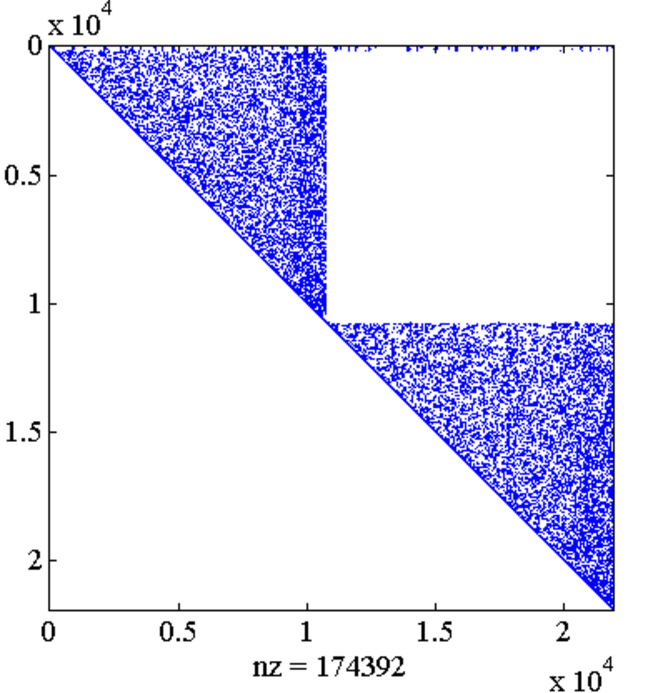
\includegraphics[width=5cm]{DDSchurMat}
}

\frame{
\frametitle{Test case of 24 cm WR90 waveguide segment }
Upper triangular part of the Schur complement matrix\\[0.2cm]
\centering
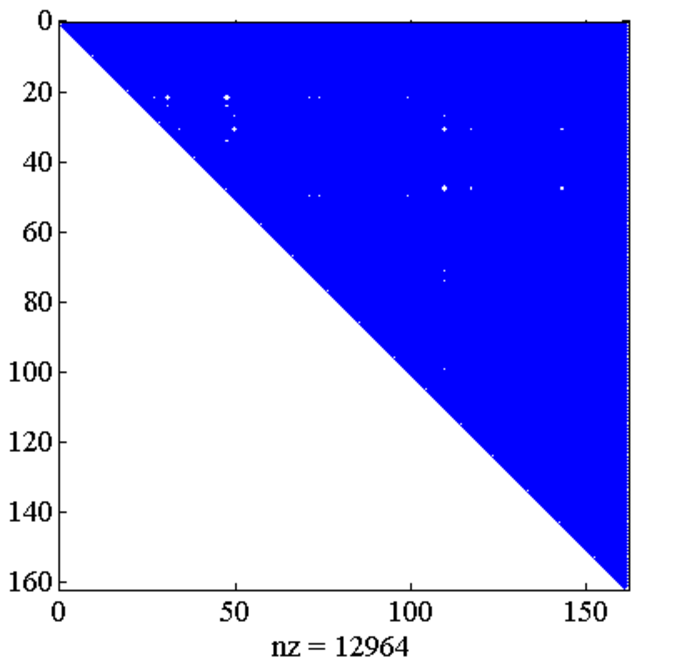
\includegraphics[width=3cm]{DDSchurMatS}
}


\frame{
\frametitle{Schur Complement based method : Critical points }
\begin{itemize}
\item The assembly of the Schur complement matrix requires the computation of large rectangular matrices $\mat{A_{jj}}^{-1} \mat{A_{\Gamma j}}^T$. One may assemble the whole Schur complement to domain $\Omega_j$, $\mat{A_{\Gamma j}} \mat{A_{jj}}^{-1} \mat{A_{\Gamma j}}^T$, upon exploiting the sparsity of $\mat{A_{\Gamma j}}^T$ and considering a few columns at a time in order to reduce the overall memory fill-in. However, if the number of unknowns pertaining to $\Omega_j$ is very large, then this step might result to be excessively time demanding.
\item The overall Schur complement matrix $\mat{S}$ is dense, and the complexity of its inversion grows dramatically with the boundary unknowns, and, consequently, with the number of subdomains.
\end{itemize}
}

\subsection{Finite Element Tearing and Interconnecting Dual-Primal domain decomposition}

\frame{
\frametitle{Finite Element Tearing and Interconnecting Dual-Primal domain decomposition }
\begin{center}
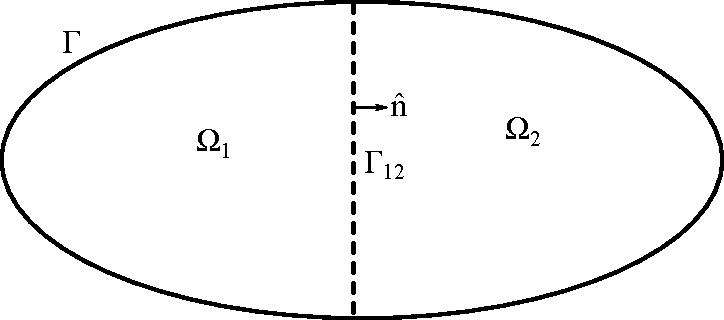
\includegraphics[width=6cm]{DDFETI}\\
\end{center}

Further unknowns are introduced to enforce fields continuity on $\Gamma_{12}$
\begin{itemize}
\item The space spanned by the sough function corresponds to \quotes{primal} unknowns 
\item The space spanned by  the boundary constrains corresponds to \quotes{dual} unknowns (coarse problem)
\end{itemize}

}

\frame{
\frametitle{FETI-DP : Model problem for $\Omega_1$ }
\small
\begin{equation*}
\label{eq:FETID1}
\left\lbrace
\begin{aligned}
\nabla \times \frac{1}{\mu_r} \nabla \times {\mathbf{E}^1} + j k_0 \zeta_0 \sigma {\mathbf{E}^1} - k_0^2 \epsilon_r {\mathbf{E}^1} = 0,& \quad \mathrm{in} \ \Omega_1\\[10pt]
\hat{\mathbf{n}} \times ( {\mathbf{E}^1} \times \hat{\mathbf{n}}) = 0, &\quad \mathrm{on} \ \mathrm{\Gamma}_E \cap d\Omega_1 \\[5pt]
\hat{\mathbf{n}} \times ( {\mathbf{H}^1} \times \hat{\mathbf{n}}) = 0, &\quad  \mathrm{on} \ \mathrm{\Gamma}_{H} \cap d\Omega_1 \\[5pt]
\hat{\mathbf{n}} \times \mathbf{H}^1 = \frac{1}{Z_s} \hat{\mathbf{n}} \times \hat{\mathbf{n}} \times \mathbf{E}^1 + \hat{\mathbf{n}} \times \mathbf{H}^{inc} - \frac{1}{Z_s} \hat{\mathbf{n}} \times \hat{\mathbf{n}} \times \mathbf{E}^{inc}, &\quad \mathrm{on} \ \Gamma_{R} \cap d\Omega_1 \\[5pt]
\hat{\mathbf{n}} \times \mathbf{H}_t^{1,k} = \frac{1}{Z_k} \hat{\mathbf{n}} \times \hat{\mathbf{n}} \times \mathbf{E}_t^{1,k} - \frac{2}{Z_k} \hat{\mathbf{n}} \times \hat{\mathbf{n}} \times \mathbf{E}_t^{k \ inc}, &\quad \mathrm{on} \ \Gamma_{WG}^k \cap d\Omega_1\\[5pt]
\hat{\mathbf{n}} \times \frac{1}{\mu_r} \nabla \times \mathbf{E}^1 - jk_0 \ \hat{\mathbf{n}} \times \mathbf{E}^1 \times \hat{\mathbf{n}} = \qquad \qquad &\\ - \hat{\mathbf{n}} \times \frac{1}{\mu_r} \nabla \times \mathbf{E}^2 - jk_0 \ \hat{\mathbf{n}} \times \mathbf{E}^2 \times \hat{\mathbf{n}},  &\quad \mathrm{on} \ \Gamma_{12} \cap d\Omega_1\\[5pt]
\end{aligned}
\right.
\end{equation*}

}

\frame{
\frametitle{FETI-DP : Model problem for $\Omega_2$ }
\small
\begin{equation*}
\label{eq:FETID2}
\left\lbrace
\begin{aligned}
\nabla \times \frac{1}{\mu_r} \nabla \times {\mathbf{E}^2} + j k_0 \zeta_0 \sigma {\mathbf{E}^2} - k_0^2 \epsilon_r {\mathbf{E}^2} = 0,& \quad \mathrm{in} \ \Omega_2\\[10pt]
\hat{\mathbf{n}} \times ( {\mathbf{E}^2} \times \hat{\mathbf{n}}) = 0,& \quad \mathrm{on} \ \mathrm{\Gamma}_E \cap d\Omega_2 \\[5pt]
\hat{\mathbf{n}} \times ( {\mathbf{H}^2} \times \hat{\mathbf{n}}) = 0,& \quad  \mathrm{on} \ \mathrm{\Gamma}_{H} \cap d\Omega_2 \\[5pt]
\hat{\mathbf{n}} \times \mathbf{H}^2 = \frac{1}{Z_s} \hat{\mathbf{n}} \times \hat{\mathbf{n}} \times \mathbf{E}^2 + \hat{\mathbf{n}} \times \mathbf{H}^{inc} - \frac{1}{Z_s} \hat{\mathbf{n}} \times \hat{\mathbf{n}} \times \mathbf{E}^{inc},& \quad \mathrm{on} \ \Gamma_{R} \cap d\Omega_2\\[5pt]
\hat{\mathbf{n}} \times \mathbf{H}_t^{2,k} = \frac{1}{Z_k} \hat{\mathbf{n}} \times \hat{\mathbf{n}} \times \mathbf{E}_t^{2,k} - \frac{2}{Z_k} \hat{\mathbf{n}} \times \hat{\mathbf{n}} \times \mathbf{E}_t^{k \ inc},& \quad \mathrm{on} \ \Gamma_{WG}^k \cap d\Omega_2\\[5pt]
\hspace{-1cm}\hat{\mathbf{n}} \times \frac{1}{\mu_r} \nabla \times \mathbf{E}^2 - jk_0 \ \hat{\mathbf{n}} \times \mathbf{E}^2 \times \hat{\mathbf{n}} = \qquad \qquad &\\ - \hat{\mathbf{n}} \times \frac{1}{\mu_r} \nabla \times \mathbf{E}^1 - jk_0 \ \hat{\mathbf{n}} \times \mathbf{E}^1 \times \hat{\mathbf{n}},& \quad \mathrm{on} \ \Gamma_{21} \cap d\Omega_2
\end{aligned}
\right.
\end{equation*}

}

\frame{
\frametitle{FETI-DP : Robin-Robin transmission condition and Galerkin framework}
The last boundary condition in each problem corresponds the \textit{Robin-Robin transmission condition}, pioneered by Despr\'es in 1991 who proved the convergence of the coarse problem restricted to boundary unknowns\\

\begin{itemize}
\item Function space
\begin{gather*}
\mathcal{W}_E^1 := \{ \mathbf{w} \in \mathcal{H}(\mathrm{curl},\Omega_1, \Gamma_E) \ | \ \hat{\mathbf{n}} \times \mathbf{w} = 0 \ \text{on} \ \Gamma_E \},\\
\mathcal{W}_E^2 := \{ \mathbf{w} \in \mathcal{H}(\mathrm{curl},\Omega_2, \Gamma_E) \ | \ \hat{\mathbf{n}} \times \mathbf{w} = 0 \ \text{on} \ \Gamma_E \},
\end{gather*}
\item Galerkin projections on $\Omega_1$
\begin{multline*}
%\label{eq:FETIform1}
\int_{\Omega_1} \nabla \times \mathbf{w}_i^* \cdot \frac{1}{\mu_r} \nabla \times \mathbf{E}^1 \ d\Omega +
 j k_0 \zeta_0 \int_{\Omega_1} \mathbf{w}_i^* \cdot \sigma \mathbf{E}^1 \ d\Omega \ - \\
 k_0^2 \int_{\Omega_1} \mathbf{w}_i^* \cdot \epsilon_r \mathbf{E}^1 \ d\Omega \ + \int_{d\Omega_1} \mathbf{w}_i^* \cdot \hat{\mathbf{n}} \times \frac{1}{\mu_r} \nabla \times {\mathbf{E}^1}  \ d\Gamma = 0, 
\quad \forall \mathbf{w}_i \in \mathcal{W}_E^1
\end{multline*}
\end{itemize}

}

\frame{
\frametitle{FETI-DP : Robin-Robin transmission condition and Galerkin framework}
\begin{itemize}
\item Galerkin projections on $\Omega_2$
\begin{multline*}
%\label{eq:FETIform2}
\int_{\Omega_2} \nabla \times \mathbf{w}_i^* \cdot \frac{1}{\mu_r} \nabla \times \mathbf{E}^2 \ d\Omega +
 j k_0 \zeta_0 \int_{\Omega_2} \mathbf{w}_i^* \cdot \sigma \mathbf{E}^2 \ d\Omega \ - \\
 k_0^2 \int_{\Omega_2} \mathbf{w}_i^* \cdot \epsilon_r \mathbf{E}^2 \ d\Omega \ + \int_{d\Omega_2} \mathbf{w}_i^* \cdot \hat{\mathbf{n}} \times \frac{1}{\mu_r} \nabla \times {\mathbf{E}^2}  \ d\Gamma = 0, 
\quad \forall \mathbf{w}_i \in \mathcal{W}_E^2
\end{multline*}
\item Transmission condition imposition: fictitious variables $\mathbf{j}^1$ and $\mathbf{j}^2$
$$
\int_{\Gamma_{12}} \mathbf{w}_i^* \cdot \hat{\mathbf{n}} \times \frac{1}{\mu_r} \nabla \times {\mathbf{E}^1}  \ d\Gamma,\quad \int_{\Gamma_{21}} \mathbf{w}_i^* \cdot \hat{\mathbf{n}} \times \frac{1}{\mu_r} \nabla \times {\mathbf{E}^2}  \ d\Gamma
$$
$$
\mathbf{j}^1  = \frac{1}{k_0} \hat{\mathbf{n}} \times \frac{1}{\mu_r} \nabla \times {\mathbf{E}^1}, \quad
\mathbf{j}^2 = \frac{1}{k_0} \hat{\mathbf{n}} \times \frac{1}{\mu_r} \nabla \times {\mathbf{E}^2}
$$
\end{itemize}

}

\frame{
\frametitle{FETI-DP : Robin-Robin transmission condition and Galerkin framework}
\begin{itemize}
\item Fictitious variables space
$$\mathcal{V}_J^i := \{ \mathbf{v} \in \mathcal{H}(\mathrm{curl},\Gamma_{ij}) \}, \quad i, j \in \lbrace1,2 \ | \ i \neq j\rbrace$$
\begin{eqnarray*}
\label{eq:auxfieldExp}
\mathbf{j}^1 &:= & \sum_{l=1}^{N^1} \lambda_j \mathbf{v}_j^1, \qquad \mathbf{v}_j^1 \in \mathcal{V}_J^1  \\
\mathbf{j}^2 &:= & \sum_{l=1}^{N^2} \lambda_j \mathbf{v}_j^2, \qquad \mathbf{v}_j^2 \in \mathcal{V}_J^2 
\end{eqnarray*}
\end{itemize}
}

\frame{
\frametitle{FETI-DP : Robin-Robin transmission condition and Galerkin framework}
\begin{eqnarray*}
\int_{\Gamma_{12}} \mathbf{w}_i^* \cdot k_0 \ \mathbf{j}^1 \ d\Gamma &= &\sum_{l=1}^{N^1} \lambda_j k_0 \int_{\Gamma_{12}} \mathbf{w}_i^* \cdot \mathbf{v}_j \ d\Gamma, \quad \forall \mathbf{w}_i \in \mathcal{W}_E^1, \ \mathbf{v}_j \in \mathcal{V}_J^1 \\
\int_{\Gamma_{21}} \mathbf{w}_i^* \cdot k_0 \ \mathbf{j}^2 \ d\Gamma &= &\sum_{l=1}^{N^2} \lambda_j k_0 \int_{\Gamma_{21}} \mathbf{w}_i^* \cdot \mathbf{v}_j \ d\Gamma, \quad \forall \mathbf{w}_i \in \mathcal{W}_E^2, \ \mathbf{v}_j \in \mathcal{V}_J^2
\end{eqnarray*}

\begin{equation*}
\label{eq:RRTC}
\left\lbrace
\begin{aligned}
j k_0 \ \mathbf{j}^1 + k_0 \ \hat{\mathbf{n}} \times \mathbf{E}^1 \times \hat{\mathbf{n}} &=  - jk_0 \ \mathbf{j}^2 + k_0 \ \hat{\mathbf{n}} \times \mathbf{E}^2 \times \hat{\mathbf{n}},& \quad \text{on} \ \Gamma_{12} \cap d\Omega_1\\
j k_0 \ \mathbf{j}^2 + k_0 \ \hat{\mathbf{n}} \times \mathbf{E}^2 \times \hat{\mathbf{n}} &=  - jk_0 \ \mathbf{j}^1 + k_0 \ \hat{\mathbf{n}} \times \mathbf{E}^1 \times \hat{\mathbf{n}},& \quad \text{on} \ \Gamma_{21} \cap d\Omega_2
\end{aligned}
\right.
\end{equation*}
}

\frame{
\frametitle{FETI-DP : Robin-Robin transmission condition and Galerkin framework}
\small
\begin{itemize}
\item Further testing with fictitious variables shape functions is performed to enforce coupling between subdomains
\begin{multline*}
j k_0 \ \int_{\Gamma_{12}} \mathbf{v}_i^* \cdot \mathbf{j}^1 \ d\Gamma + k_0 \ \int_{\Gamma_{12}} \mathbf{v}_i^* \cdot \hat{\mathbf{n}} \times \mathbf{E}^1 \times \hat{\mathbf{n}} \ d\Gamma = \\
- jk_0 \ \int_{\Gamma_{12}} \mathbf{v}_i^* \cdot \mathbf{j}^2 \ d\Gamma + k_0 \
\int_{\Gamma_{12}} \mathbf{v}_i^* \cdot \hat{\mathbf{n}} \times \mathbf{E}^2 \times \hat{\mathbf{n}} \ d\Gamma, \quad \forall \mathbf{v}_i \in \mathcal{V}_J^1
\end{multline*}
\begin{multline*}
jk_0 \ \int_{\Gamma_{21}} \mathbf{v}_i^* \cdot \mathbf{j}^2 \ d\Gamma + k_0 \ \int_{\Gamma_{21}} \mathbf{v}_i^* \cdot \hat{\mathbf{n}} \times \mathbf{E}^2 \times \hat{\mathbf{n}} \ d\Gamma = \\
- jk_0 \ \int_{\Gamma_{21}} \mathbf{v}_i^* \cdot \mathbf{j}^1 \ d\Gamma + k_0 \
\int_{\Gamma_{21}} \mathbf{v}_i^* \cdot \hat{\mathbf{n}} \times \mathbf{E}^1 \times \hat{\mathbf{n}} \ d\Gamma, \quad \forall \mathbf{v}_i \in \mathcal{V}_J^2
\end{multline*}
\end{itemize}
}

\frame{
\frametitle{FETI-DP : Subsystems matrices}
\small
\begin{equation*}
\begin{bmatrix}
A_{11} & A_{\Gamma_1 1} & \\
A_{\Gamma_1 1}^T & A_{\Gamma_1 \Gamma_1} & D_{11}\\
 & D_{11}^T  & T_{11}
\end{bmatrix}
\begin{bmatrix}
x_{1}\\
x_{\Gamma_1}\\
\lambda_{1}
\end{bmatrix}
=
\begin{bmatrix}
B_{1}\\
B_{\Gamma_1}\\
\phantom{x}
\end{bmatrix}
+
\begin{bmatrix}
\phantom{-}\phantom{A} & \phantom{-}\phantom{A} & \phantom{A}\\
\phantom{A} & \phantom{A} & \phantom{A}\\
\phantom{A} & D_{12}  & -T_{12}
\end{bmatrix}
\begin{bmatrix}
\phantom{A}\\
x_{\Gamma_2}\\
\lambda_{2}
\end{bmatrix}
\end{equation*}

\begin{equation*}
\begin{bmatrix}
A_{22} & A_{\Gamma_2 2} & \\
A_{\Gamma_2 2}^T & A_{\Gamma_2 \Gamma_2} & D_{22}\\
 & D_{22}^T  & T_{22}
\end{bmatrix}
\begin{bmatrix}
x_{2}\\
x_{\Gamma_2}\\
\lambda_{1}
\end{bmatrix}
=
\begin{bmatrix}
B_{2}\\
B_{\Gamma_2}\\
\phantom{x}
\end{bmatrix}
+
\begin{bmatrix}
\phantom{-}\phantom{A} & \phantom{-}\phantom{A} & \phantom{A}\\
\phantom{A} & \phantom{A} & \phantom{A}\\
\phantom{A} & D_{21}  & -T_{21}
\end{bmatrix}
\begin{bmatrix}
\phantom{x}\\
x_{\Gamma_1}\\
\lambda_{1}
\end{bmatrix}
\end{equation*}

\begin{gather*}
D_{mm} = k_0 \ \int_{\Gamma_{mn}} {\mathbf{v}_i^{m}}^* \cdot \hat{\mathbf{n}} \times\mathbf{w}_j^m \times \hat{\mathbf{n}} \ d\Gamma, \\
T_{mm} = jk_0 \ \int_{\Gamma_{mn}} {\mathbf{v}_i^{m}}^* \cdot \mathbf{v}_j^m \ d\Gamma,\\
D_{mn} = k_0 \ \int_{\Gamma_{mn}} {\mathbf{v}_i^{m}}^* \cdot \hat{\mathbf{n}} \times\mathbf{w}_j^n \times \hat{\mathbf{n}} \ d\Gamma, \\
T_{mn} = jk_0 \ \int_{\Gamma_{mn}} {\mathbf{v}_i^{m}}^* \cdot \mathbf{v}_j^n \ d\Gamma.
\end{gather*}
}

\frame{
\frametitle{FETI-DP : Coarse problem restriction}
Memory saving upon storing only boundary unknowns by the use of a \underline{restriction matrix}
\small
$$ \mat{R}_1 = \begin{bmatrix}
\phantom{I_{P_1}} & I_{P_1} & \\
& & I_{D_1}
\end{bmatrix}$$
For $\Omega_1$ :
\begin{multline*}
\begin{bmatrix}
x_{\Gamma_1}\\
\lambda_{1}
\end{bmatrix} =
\mat{R}_1
\begin{bmatrix}
x_{1}\\
x_{\Gamma_1}\\
\lambda_{1}
\end{bmatrix}
=\\
\mat{R}_1
\begin{bmatrix}
A_{11} & A_{\Gamma_1 1} & \\
A_{\Gamma_1 1}^T & A_{\Gamma_1 \Gamma_1} & D_{11}\\
 & D_{11}^T  & T_{11}
\end{bmatrix}^{-1}
\left(
\begin{bmatrix}
B_{1}\\
B_{\Gamma_1}\\
\phantom{x}
\end{bmatrix}
+
\begin{bmatrix}
\phantom{-}\phantom{A} & \phantom{-}\phantom{A} & \phantom{A}\\
\phantom{A} & \phantom{A} & \phantom{A}\\
\phantom{A} & D_{12}  & -T_{12}
\end{bmatrix}
\begin{bmatrix}
\phantom{x}\\
x_{\Gamma_2}\\
\lambda_{2}
\end{bmatrix}
\right) = \\
\underbrace{
\mat{R}_1
\begin{bmatrix}
A_{11} & A_{\Gamma_1 1} & \\
A_{\Gamma_1 1}^T & A_{\Gamma_1 \Gamma_1} & D_{11}\\
 & D_{11}^T  & T_{11}
\end{bmatrix}^{-1}
}_{(1)}
\left(
\begin{bmatrix}
B_{1}\\
B_{\Gamma_1}\\
\phantom{x}
\end{bmatrix}
+
\begin{bmatrix}
\phantom{A} & \phantom{A}\\
\phantom{A} & \phantom{A}\\
D_{12}  & -T_{12}
\end{bmatrix}
\begin{bmatrix}
x_{\Gamma_2}\\
\lambda_{2}
\end{bmatrix}
\right).
\end{multline*}
(1) small but dense rectangular matrix that can be stored
}

\frame{
\frametitle{Test case of 24 cm WR90 waveguide segment}
Convergence history of the restricted FETI-DP algorithm at 10~GHz and spectral response\\[.2cm]
\centering
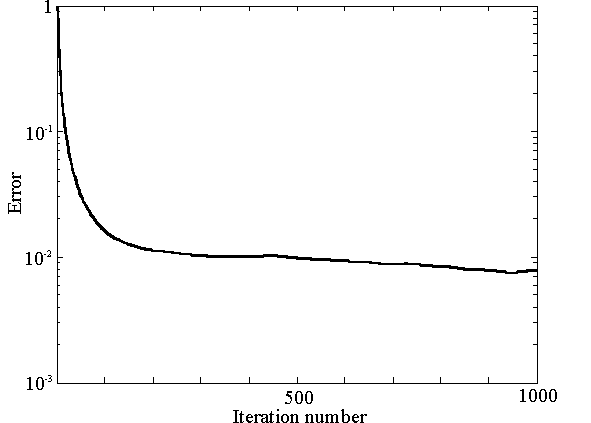
\includegraphics[width=5.5cm]{Convergence} \ 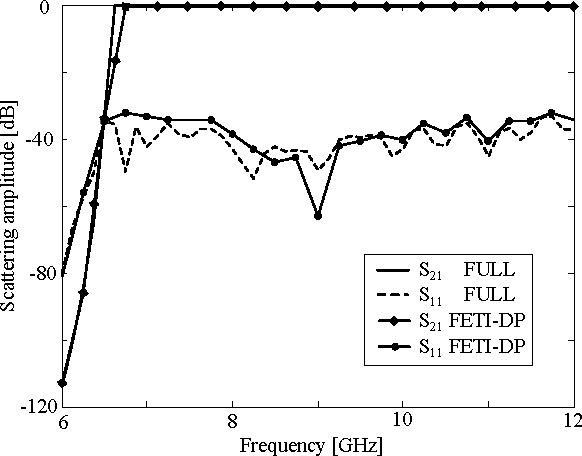
\includegraphics[width=5cm]{WRfreqFETI}\\
430 iterations ($\approx 200~\text{s}$) to achieve an error of $10^{-2}$ \\ $\rightarrow$ 2.1~\% relative error on the spectral response
}

\frame{
\frametitle{FETI-DP : Critical points }
\begin{itemize}
\item The poor convergence behavior is due to a non-optimal residual minimization. This result has motivated the use of the FETI-DP as a preconditioner for Krylov iterative solvers which not only guarantee the convergence of the solution, but somehow choose the best directions
\end{itemize}
}

\frame{
\frametitle{FETI-DP : Full system assembly for iterative solvers}
\begin{equation*}
\label{eq:FETIDPFull}
\begin{bmatrix}
A_{11} & A_{\Gamma_1 1} & & & & \\
A_{\Gamma_1 1}^T & A_{\Gamma_1 \Gamma_1} & D_{11} & & &\\
 & D_{11}^T  & T_{11} & \phantom{A} & -D_{12}  & T_{12}\\
& & & A_{22} & A_{\Gamma_2 2} &  \\
& & & A_{\Gamma_2 2}^T & A_{\Gamma_2 \Gamma_2} & D_{22}\\
\phantom{A} & -D_{21}  & T_{21} & & D_{22}^T  & T_{22}
\end{bmatrix}
\begin{bmatrix}
x_{1}\\
x_{\Gamma_1}\\
\lambda_{1}\\
x_{2}\\
x_{\Gamma_2}\\
\lambda_{2}
\end{bmatrix}
=
\begin{bmatrix}
\phantom{x}\\
B_{\Gamma_1}\\
\phantom{x}\\
\phantom{x}\\
B_{\Gamma_2}\\
\phantom{x}\\
\end{bmatrix}
\end{equation*}
}

\subsection{Domain decomposition based preconditioners}

\frame{
\frametitle{Domain decomposition based preconditioners}
Given a block-wise system matrix
\begin{equation*}
\label{eq:SysBlocks}
\begin{bmatrix}
A_{11} & A_{12} & A_{13}\\
A_{21} & A_{22} & A_{23}\\
A_{31} & A_{32} & A_{33}
\end{bmatrix}
\begin{bmatrix}
x_{1}\\
x_{2}\\
x_{3}
\end{bmatrix}
=
\begin{bmatrix}
b_{1}\\
b_{2}\\
b_{3}
\end{bmatrix}
\end{equation*}
one can build preconditioners that exploits block matrix inversion
\begin{itemize}
\item Jacobi preconditioner
\item Gauss-Seidel preconditioner
\end{itemize}
that can readily be merge into an iterative solver (GMRES)
}

\frame{
\frametitle{Domain decomposition based preconditioners : Jacobi}
$$ 
\mat{P}_{J}^{-1} = 
\begin{bmatrix}
A_{11} &  & \\
 & A_{22} & \\
 & & A_{33}
\end{bmatrix}^{-1} = 
\begin{bmatrix}
\mat{A_{11}}^{-1} &  & \\
 & \mat{A_{22}}^{-1} & \\
 & & \mat{A_{33}}^{-1}
\end{bmatrix}
$$
}
\frame{
\frametitle{Domain decomposition based preconditioners : Gauss-Seidel}
\begin{gather*}
\mat{P}_{GS}^{-1} = 
\begin{bmatrix}
A_{11} &  & \\
A_{21} & A_{22} & \\
A_{31} & A_{32} & A_{33}
\end{bmatrix}^{-1} = 
\begin{bmatrix}
\mat{A_{11}}^{-1} &  & \\
\tilde{\mat{A_{21}}} & \mat{A_{22}}^{-1} & \\
\tilde{\mat{A_{31}}} & \tilde{\mat{A_{32}}} & \mat{A_{33}}^{-1}
\end{bmatrix}
\end{gather*}
\noindent where
\begin{eqnarray*}
\tilde{\mat{A_{21}}} &= &-\mat{A_{22}}^{-1}\mat{A_{21}}\mat{A_{11}}^{-1}\\
\tilde{\mat{A_{32}}} &= &-\mat{A_{33}}^{-1} \mat{A_{32}} \mat{A_{22}}^{-1}\\
\tilde{\mat{A_{31}}} &= &\mat{A_{33}}^{-1}\mat{A_{32}}\mat{A_{22}}^{-1}\mat{A_{21}}\mat{A_{11}}^{-1}- \mat{A_{33}}^{-1}\mat{A_{31}}\mat{A_{11}}^{-1}
\end{eqnarray*}
A sequential procedure can be employed to apply the preconditioner to the residual vector of the iterative solver
}

\frame{
\frametitle{Domain decomposition based preconditioners : Performances}
\centering
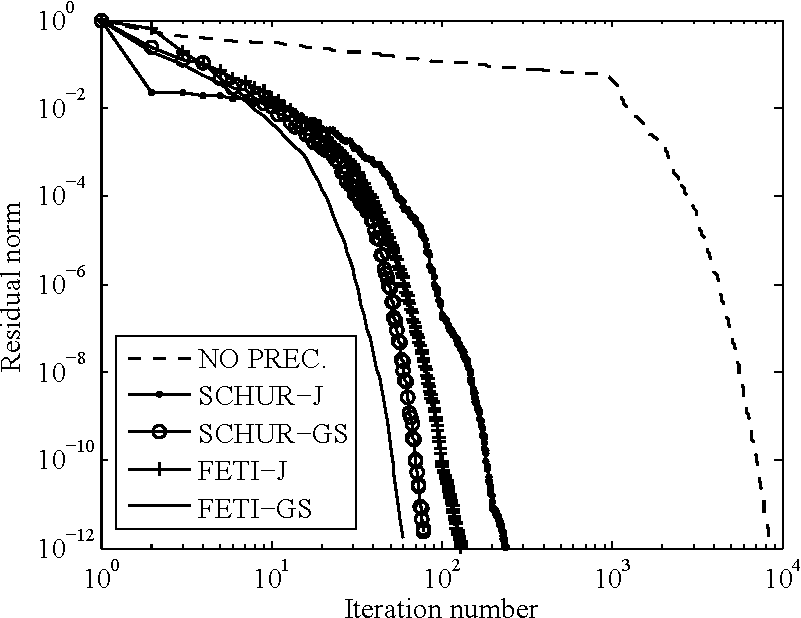
\includegraphics[width=7cm]{GMREScomp}
}

\frame{
\frametitle{Domain decomposition based preconditioners : Performances}
Times and memory requirements for different GMRES(100) runs at 10~GHz\\[.2cm]
\centering
\begin{table}[h!]
\begin{center}
\begin{tabular}{|c|c|c|c|}
\hline 
Solver & Iterations & Time & Peak memory \\ 
\hline
\hline 
Direct (double precision) & - & 1~s & 49.5~MB\\ \hline 
No preconditioner & 8459 & 276~s & 68.2~MB\\ \hline 
DD-Schur Jacobi precond. & 238 & 160~s & 68.6~MB\\ \hline 
DD-Schur Gauss-Seidel precond. & 78 & 54.5~s & 69.1~MB\\ \hline 
DD-FETI Jacobi precond. & 130 & 90~s & 69.7~MB\\ \hline 
DD-FETI Gauss-Seidel precond. & 58 & 41.8~s & 69.2~MB\\ \hline 
\end{tabular}
\end{center}
\label{tab:gmresComp}
\end{table}
}

\frame{
\frametitle{Domain decomposition based preconditioners : Performances}
Comparison between the SCHUR and FETI Gauss-Seidel preconditioned GMRES(100) runs as the frequency of excitation varies\\[.2cm]
\centering
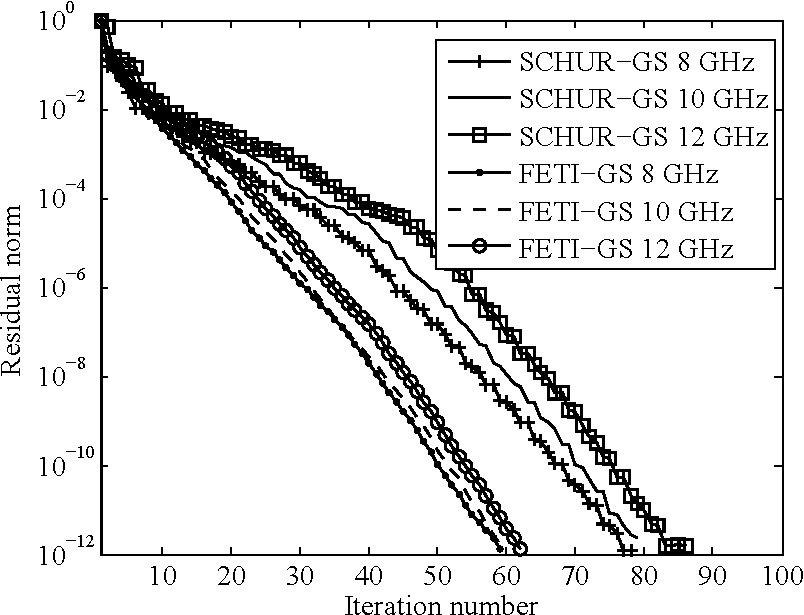
\includegraphics[width=7cm]{DDfreqComp}
}

\frame{
\frametitle{Domain decomposition based preconditioners : Performances}
Convergence history for SCHUR-GS GMRES(100) solution at 10~GHz with either dominant mode or transfinite element method waveports boundary conditions\\[.2cm]
\centering
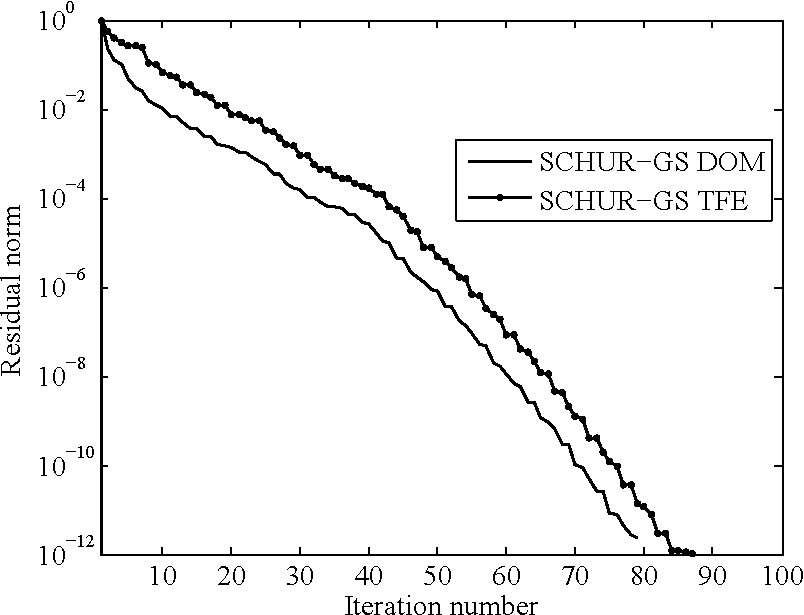
\includegraphics[width=7cm]{schurdomtfe}
}


\frame{
\frametitle{Domain decomposition based preconditioners : Performances}
Scattering parameters accuracy for different prescribed residual errors (runs at 10~GHz with dominant mode on waveports)\\[.2cm]
\centering
\scriptsize
\begin{table}[h]
\begin{center}
\begin{tabular}{|c|c|c|c|c|}
\hline 
Solver & Residual error & $|S_{11}|$~[dB] & $|S_{21}|$~[dB] & $\frac{\Vert |S_\mathrm{ref}| - |S| \Vert_{2}}{\Vert|S_\mathrm{ref}|\Vert_2}$\\ 
\hline
\hline 
Direct (reference) & - & -42.8389 & -0.0024 & 0\\ \hline \hline
\setlength{\arrayrulewidth}{0.5pt}
DD-Schur Gauss-Seidel & $10^{-2}$ & -26.7529 & -0.1958 & $2.23~10^{-2}$\\ \hline 
"& $10^{-4}$ & -42.5118 & -0.0030 & $1.4234~10^{-4}$\\ \hline 
"& $10^{-6}$ & -42.8397 & -0.0025 & $4.0786~10^{-7}$\\ \hline 
"& $10^{-8}$ & -42.8389 & -0.0024 & $3.4517~10^{-9}$\\ \hline 
"& $10^{-10}$ & -42.8389 & -0.0024 & $8.2561~10^{-11}$\\ \hline
"& $10^{-12}$ & -42.8389 & -0.0024 & $1.2571~10^{-13}$\\ \hline \hline
DD-FETI Gauss-Seidel & $10^{-2}$ & -40.5331 & -0.0603 & $3.5~10^{-3}$\\ \hline 
"& $10^{-4}$ & -42.8404 & -0.0024 & $2.0280~10^{-6}$\\ \hline 
"& $10^{-6}$ & -42.8389 & -0.0024 & $1.1615~10^{-8}$\\ \hline 
"& $10^{-8}$ & -42.8389 & -0.0024 &  $5.5698~10^{-10}$\\ \hline 
"& $10^{-10}$ & -42.8389 & -0.0024 & $1.8771~10^{-12}$\\ \hline
"& $10^{-12}$ & -42.8389 & -0.0024 & $1.7357~10^{-14}$\\ \hline
\end{tabular}
\end{center}
%\caption{Scattering parameters accuracy for different prescribed residual errors (runs at 10~GHz with dominant mode on waveports).}
\label{tab:Sacc}
\end{table}
}

\frame{
\frametitle{Domain decomposition based preconditioners : Performances}
Scattering parameters accuracy for different prescribed residual errors (runs at 10~GHz with transfinite elements on waveports)\\[.2cm]
\centering
\scriptsize
\begin{table}[h]
\begin{center}
\begin{tabular}{|c|c|c|c|c|}
\hline 
Solver & Residual error & $|S_{11}|$~[dB] & $|S_{21}|$~[dB] & $\frac{\Vert |S_\mathrm{ref}| - |S| \Vert_{2}}{\Vert|S_\mathrm{ref}|\Vert_2}$\\ 
\hline
\hline 
Direct (reference) & - & -42.8035  & -0.0002 & 0\\ \hline \hline
\setlength{\arrayrulewidth}{0.5pt}
DD-Schur Gauss-Seidel & $10^{-2}$ & -35.1814  & -0.0682 & $6.4~10^{-3}$\\ \hline 
"& $10^{-4}$ & -42.7897 &  -0.0002 & $6.8925~10^{-6}$\\ \hline 
"& $10^{-6}$ & -42.8034 &  -0.0002 & $1.3365~10^{-7}$\\ \hline 
"& $10^{-8}$ & -42.8035 &  -0.0002 & $3.9561~10^{-10}$\\ \hline
"& $10^{-10}$ & -42.8035 &  -0.0002 & $8.2355~10^{-12}$\\ \hline
"& $10^{-12}$ & -42.8035 &  -0.0002 & $2.0021~10^{-13}$\\ \hline
\end{tabular}
\end{center}
%\caption{Scattering parameters accuracy for different prescribed residual errors (runs at 10~GHz with transfinite elements on waveports).}
\label{tab:SaccTFE}
\end{table}
}

\frame{
\frametitle{DD based preconditioners : Performances against subdomains number}
Rectangular waveguide partitionned in 4, 8, 12 and 16 subdomains with Metis\\[.2cm]
\centering
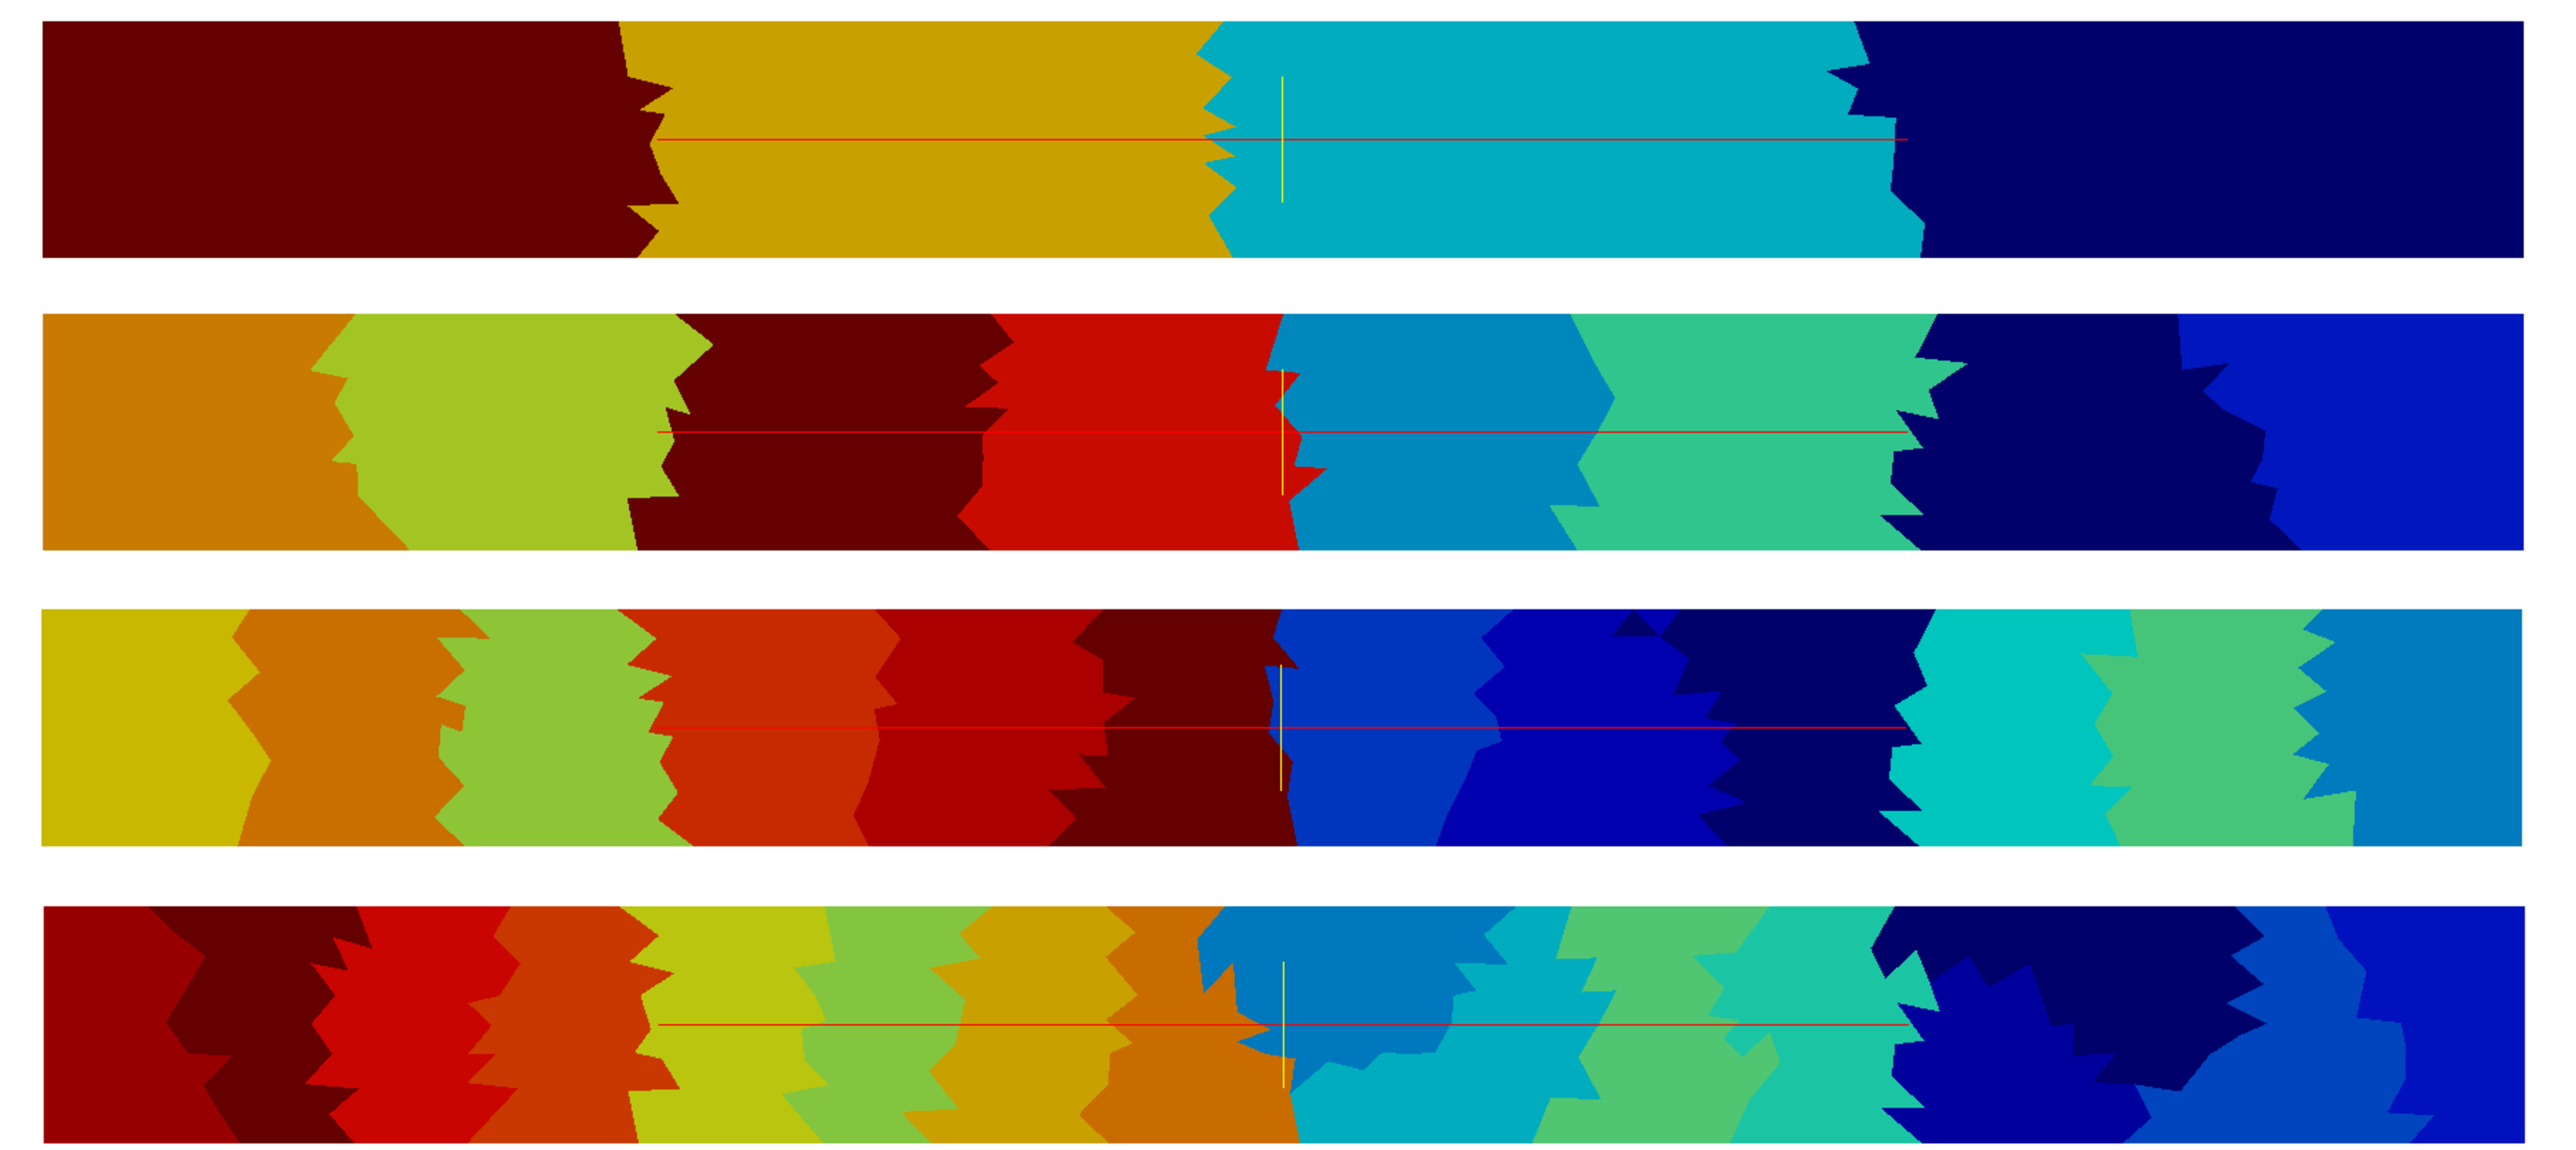
\includegraphics[width=8cm]{Partitions}
}

\frame{
\frametitle{DD based preconditioners : Performances against subdomains number}
Scattering parameters accuracy for different prescribed residual errors (runs at 10~GHz) when edge corners are avoided\\[.2cm]
\centering
\begin{table}[h]
\begin{center}
\begin{tabular}{|c|c|c|}
\hline 
Solver (Nbr of Tetrahedra) & Nbr. of Sub-domains & $\frac{\Vert |S_\mathrm{ref}| - |S| \Vert_{2}}{\Vert|S_\mathrm{ref}|\Vert_2}$\\ 
\hline \hline 
\setlength{\arrayrulewidth}{0.5pt}
SCHUR (20~602) & 4 & $1.5926~10^{-6}$\\ \hline 
"& 8 & $5.95814~10^{-6}$\\ \hline 
"& 12 &  $3.29779~10^{-5}$\\ \hline 
"& 16 & $2.96923~10^{-4}$\\ \hline
FETI (20~602) & 4 & $2.14849~10^{-6}$\\ \hline 
"& 8  & $5.48124~10^{-6}$\\ \hline 
"& 12 & $1.02953~10^{-5}$\\ \hline 
"& 16 & $5.93607~10^{-3}$\\ \hline
SCHUR (25~093) & 16 & $8.29628~10^{-6}$\\ \hline 
FETI (25~093) & 16 & $1.90617~10^{-6}$\\ \hline 
\end{tabular}
\end{center}
\label{tab:SaccDDSweep}
\end{table}
}

\frame{
\frametitle{DD based preconditioners : Performances against subdomains number}
Scattering parameters accuracy for different prescribed residual errors (runs at 10~GHz) when edge corners are avoided\\[.2cm]
\centering
\begin{table}[h]
\begin{center}
\begin{tabular}{|c|c|c|}
\hline 
Solver (Nbr of Tetrahedra) & Nbr. of Sub-domains & $\frac{\Vert |S_\mathrm{ref}| - |S| \Vert_{2}}{\Vert|S_\mathrm{ref}|\Vert_2}$\\ 
\hline \hline 
\setlength{\arrayrulewidth}{0.5pt}
SCHUR (20~602) & 4 & $1.5926~10^{-6}$\\ \hline 
"& 8 & $5.95814~10^{-6}$\\ \hline 
"& 12 &  $3.29779~10^{-5}$\\ \hline 
"& 16 & $2.96923~10^{-4}$\\ \hline
FETI (20~602) & 4 & $2.14849~10^{-6}$\\ \hline 
"& 8  & $5.48124~10^{-6}$\\ \hline 
"& 12 & $1.02953~10^{-5}$\\ \hline 
"& 16 & $5.93607~10^{-3}$\\ \hline
SCHUR (25~093) & 16 & $8.29628~10^{-6}$\\ \hline 
FETI (25~093) & 16 & $1.90617~10^{-6}$\\ \hline 
\end{tabular}
\end{center}
\label{tab:SaccDDSweep}
\end{table}
}

\frame{
\frametitle{DD based preconditioners : Performances against subdomains number}
Convergence histories for SCHUR and FETI GMRES(100) solvers as the number of subdomains is increased, respectively to TFE and DOM full analyzes at 10~GHz on relative mesh\\[.2cm]
\centering
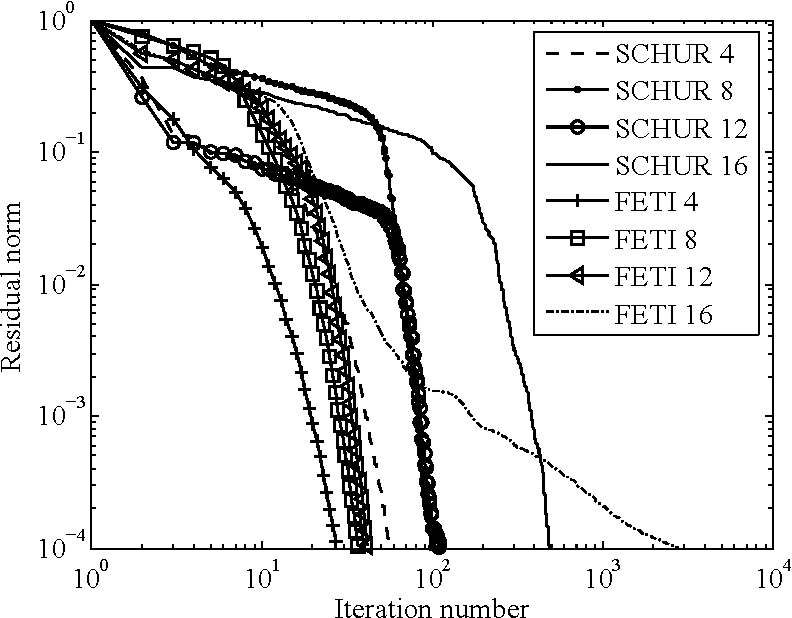
\includegraphics[width=7cm]{DDsweep}
}

\frame{
\frametitle{DD based preconditioners : Performances against subdomains number}
The two different meshes of the rectangular waveguide both partitioned in 16 subdomains. Top to bottom: 20~602 and 25~093 tetrahedra\\[.2cm]
\centering
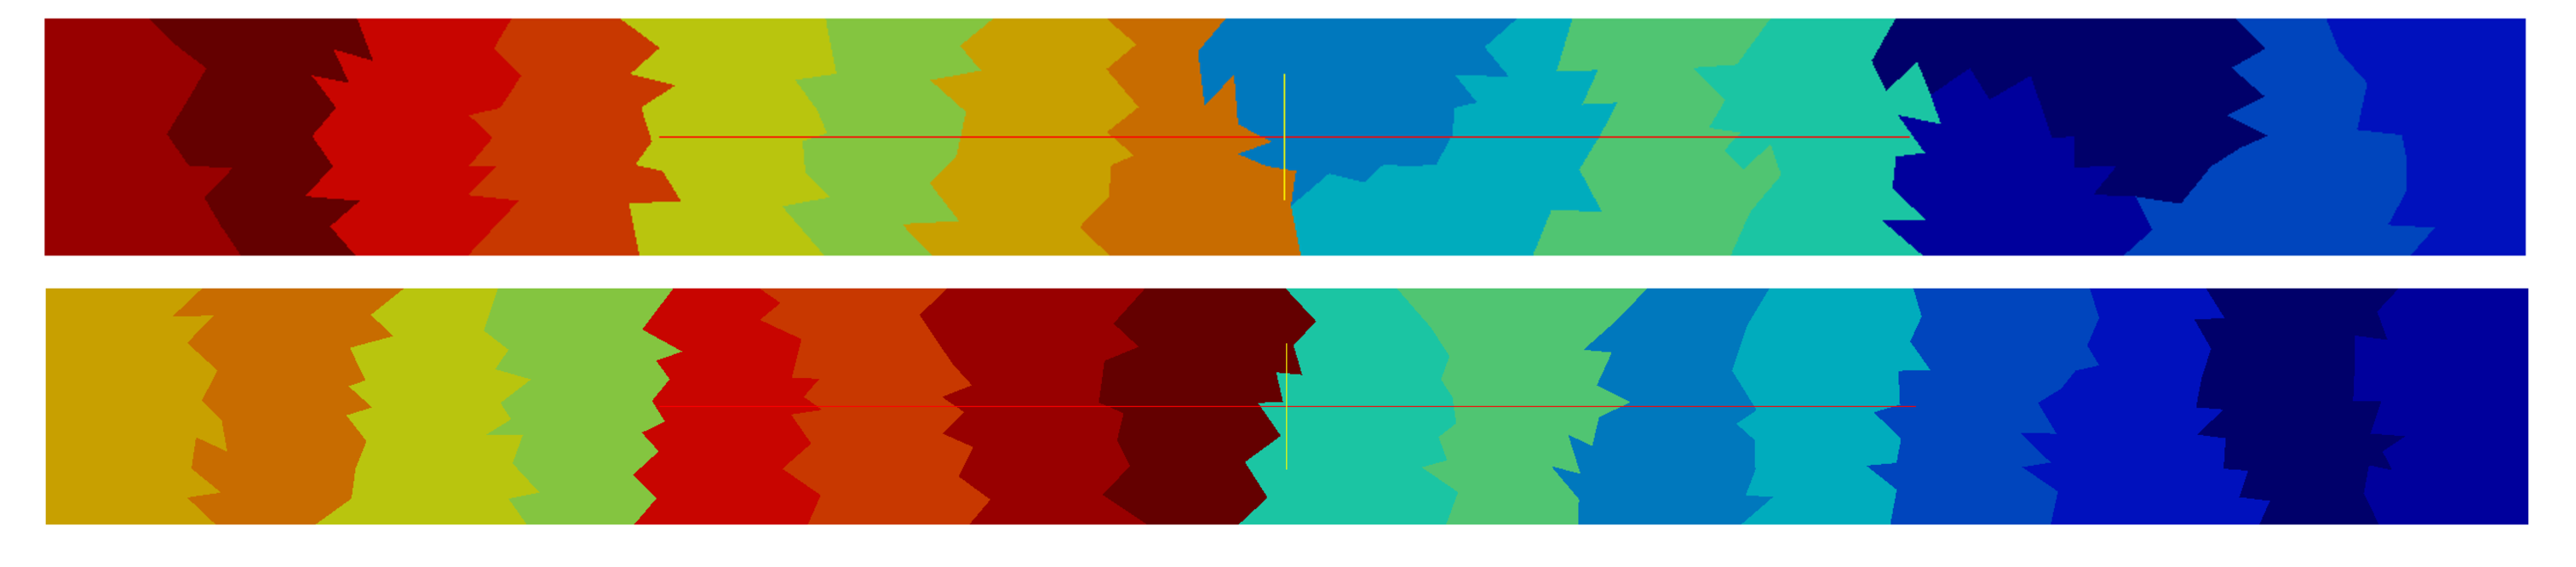
\includegraphics[width=9cm]{Partitions2}
}

\frame{
\frametitle{DD based preconditioners : Performances against subdomains number}
Convergence histories for SCHUR and FETI GMRES(100) solvers on initial (20~602 tetrahedra) and refined (25~093 tetrahedra) meshes partitioned in 16 subdomains\\[.2cm]
\centering
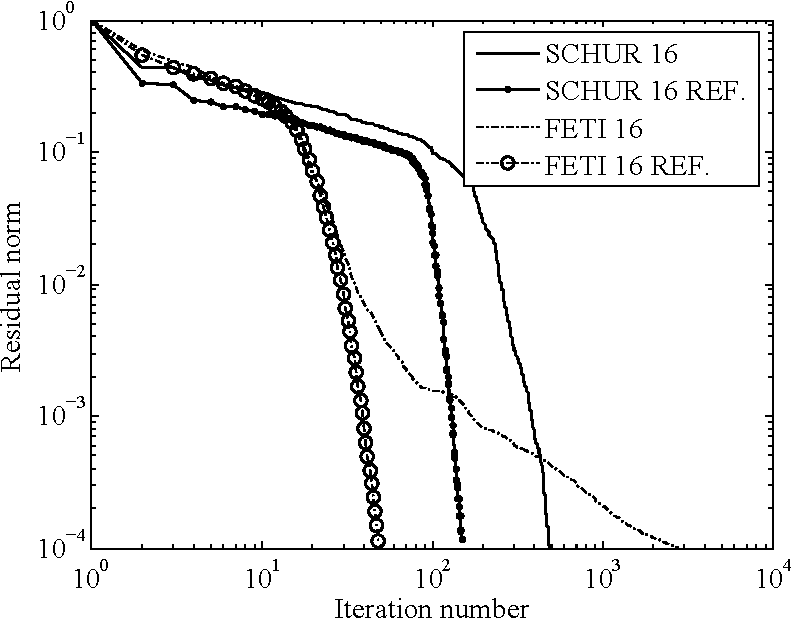
\includegraphics[width=7cm]{DD16ref}
}


\frame{
\frametitle{Direct solvers : Performances against problem size}
CPU time and memory consumption for different problem sizes analyzed with FES employing the double precision sparse direct solver\\[.2cm]
\centering
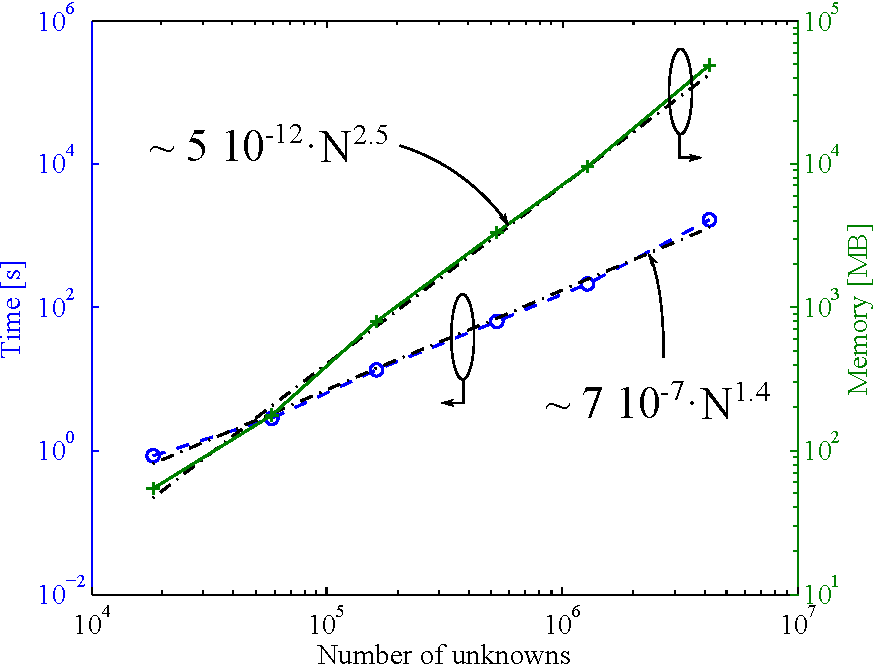
\includegraphics[width=7cm]{DirectCompl}
}

\frame{
\frametitle{DD based preconditioners : Performances against problem size}
CPU time and memory consumption for different problem sizes analyzed with FES employing the GMRES(100) FETI-DP GS preconditioned solver\\[.2cm]
\centering
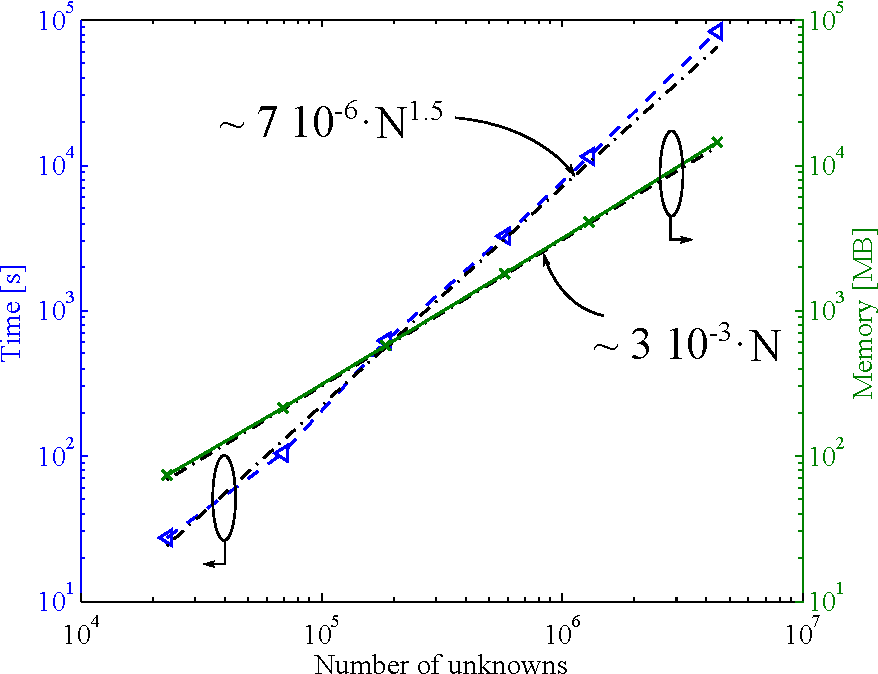
\includegraphics[width=7cm]{IterCompl}
}

\frame{
\frametitle{DD based preconditioners : Performances against problem size}
\begin{itemize}
\item Gauss-Seidel preconditioned GMRES solver results to be promising for very large problems
\item Corner edges remain a critical point that still have to be tackled in the preprocessing phase
\end{itemize}
}

\graphicspath{{img/ch3/}}

\section{Nonlinear Analysis of Passive Microwave Devices}

\subsection{Harmonic balance finite elements}

\frame{
\frametitle{Multiport devices with nonlinear materials}
\centering
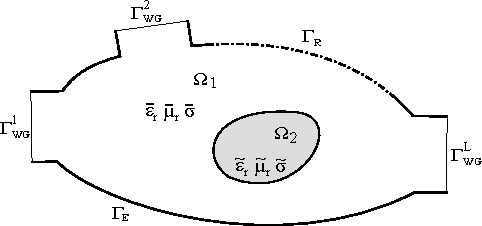
\includegraphics[width=7cm]{geometryLarge}
\small
\begin{gather*}
\epsilon_r(\mathbf{E}(\mathbf{r}),\mathbf{r}) = 
\begin{cases}
\bar{\epsilon}_r(\mathbf{r}), & \mathbf{r} \in \Omega_1  \\
\tilde{\epsilon}_r(\mathbf{E}(\mathbf{r}), \mathbf{r}) \!=\!
\bar{\epsilon}_r(\mathbf{r}) \!+\! \mathcal{N}_\epsilon(\mathbf{E}(\mathbf{r})), & \mathbf{r} \in
\Omega_2
\end{cases} \label{eq:epsnl}\\
\mu_r^{-1}(\mathbf{H}(\mathbf{r}),\mathbf{r}) = \nu_r(\mathbf{H}(\mathbf{r}),\mathbf{r}) = 
\begin{cases}
\bar{\nu}_r(\mathbf{r}), & \mathbf{r} \in \Omega_1 \\
\tilde{\nu}_r(\mathbf{H}(\mathbf{r}), \mathbf{r}) \!=\!
\bar{\nu}_r(\mathbf{r}) \!+\! \mathcal{N}_\nu(\mathbf{H}(\mathbf{r})), & \mathbf{r} \in
\Omega_2
\end{cases}\label{eq:munl}\\
\sigma(\mathbf{E}(\mathbf{r}),\mathbf{r}) = 
\begin{cases}
\bar{\sigma}(\mathbf{r}), & \mathbf{r} \in \Omega_1\\
\tilde{\sigma}(\mathbf{E}(\mathbf{r}), \mathbf{r}) \!=\!
\bar{\sigma}(\mathbf{r}) \!+\! \mathcal{N}_\sigma(\mathbf{E}(\mathbf{r})), & \mathbf{r} \in
\Omega_2
\end{cases}\label{eq:signl}
\end{gather*}
}

\frame{
\frametitle{Multiport devices with nonlinear materials: Conventional Galerkin framework}
\small
\begin{multline*}
\nabla \times \nu_r(\mathbf{H}(\mathbf{r}),\mathbf{r}) \ \nabla \times {\mathbf{E}(\mathbf{r})} \ +\\  j k_0 \zeta_0 \sigma(\mathbf{E}(\mathbf{r}),\mathbf{r}) \ {\mathbf{E}(\mathbf{r})} \ - k_0^2 \epsilon_r(\mathbf{E}(\mathbf{r}),\mathbf{r}) \ {\mathbf{E}(\mathbf{r})} = 0
\end{multline*}
$$\Downarrow$$
\begin{multline*}
\int_\Omega \nabla \times \mathbf{w}_i^*(\mathbf{r}) \cdot \nu_r(\mathbf{H}(\mathbf{r}),\mathbf{r}) \nabla \times \mathbf{E}(\mathbf{r}) \ d\Omega \ + \\
 \hspace{-5cm} j k_0 \zeta_0 \int_\Omega \mathbf{w}_i^*(\mathbf{r}) \cdot \sigma(\mathbf{E}(\mathbf{r}),\mathbf{r}) \ \mathbf{E}(\mathbf{r}) \ d\Omega \ - \\
 \hspace{-3cm} k_0^2 \int_\Omega \mathbf{w}_i^*(\mathbf{r}) \cdot \epsilon_r(\mathbf{E}(\mathbf{r}),\mathbf{r}) \ \mathbf{E}(\mathbf{r}) \ d\Omega \ = \\
\int_{\Gamma} \mathbf{w}_i^*(\mathbf{r})  \times \nu_r(\mathbf{H}(\mathbf{r}),\mathbf{r}) \nabla \times {\mathbf{E}}(\mathbf{r}) \cdot \hat{\mathbf{n}} \ d\Gamma, 
\quad \forall \mathbf{w}_i(\mathbf{r}) \in \mathcal{W}_E.
\end{multline*}
}


\frame{
\frametitle{HBFE: Multiharmonic dependence of the fields}
\begin{equation*} \label{eq:field}
\hat{\mathcalb{E}}(\mathbf{r}, t) = \sum^P_{p=1} \left( \mathbf{E}_{p}^{(s)}(\mathbf{r}) \sin(p
\omega_0 t) + \mathbf{E}_p^{(c)}(\mathbf{r}) \cos(p \omega_0 t) \right)
\end{equation*} 
$$
\mathbf{E}_{p}^{(s)}(\mathbf{r}) := \sum_{j=1}^{N} x_j^{(s)} \mathbf{w}_j(\mathbf{r}), \qquad \mathbf{w}_j(\mathbf{r}) \in \mathcal{W}_E
$$ 
$$
\mathbf{E}_{p}^{(c)}(\mathbf{r}) := \sum_{j=1}^{N} x_j^{(c)} \mathbf{w}_j(\mathbf{r}), \qquad \mathbf{w}_j(\mathbf{r}) \in \mathcal{W}_E
$$

}

\frame{
\frametitle{HBFE: Multiharmonic dependence of materials}
\small
\begin{gather*} \label{eq:matfourier}
\hat{{\epsilon}}_r(\mathbf{E}(\mathbf{r}), \mathbf{r}, t) = {\epsilon}_{r_0}(\mathbf{E}(\mathbf{r}),\mathbf{r}) \ +
\sum^{G_\epsilon}_{g=1} {\epsilon}_{r_g}^{(s)}(\mathbf{E}(\mathbf{r}),\mathbf{r}) \sin(g \omega_0 t) + \ \\ \sum^{G_\epsilon}_{g=1}  {\epsilon}_{r_g}^{(c)}(\mathbf{E}(\mathbf{r}),\mathbf{r}) \cos(g \omega_0 t)
\end{gather*} 

\begin{equation*}
\left\{
\begin{aligned} \label{eq:epsCoeffs}
{\epsilon}_{r_{0}}(\mathbf{E}(\mathbf{r}),\mathbf{r}) &= \frac{\omega_0}{2\pi}\int_0^{\frac{2\pi}{\omega_0}}
{\epsilon}_r(\mathbf{E}(\mathbf{r}),\mathbf{r}) \ dt, \\[.5cm]
{\epsilon}_{r_{g}}^{(s)}(\mathbf{E}(\mathbf{r}),\mathbf{r}) &=  \frac{\omega_0}{\pi}\int_0^{\frac{2\pi}{\omega_0}}
{\epsilon}_r(\mathbf{E}(\mathbf{r}),\mathbf{r}) \ \sin(g \omega_0 t) \ dt, \\[.5cm]
{\epsilon}_{r_{g}}^{(c)}(\mathbf{E}(\mathbf{r}),\mathbf{r}) &=  \frac{\omega_0}{\pi}\int_0^{\frac{2\pi}{\omega_0}} 
{\epsilon}_r(\mathbf{E}(\mathbf{r}),\mathbf{r}) \ \cos(g \omega_0 t) \ dt,
\end{aligned}
\right.
\end{equation*}
}

\frame{
\frametitle{HBFE: Multiharmonic dependence of materials}
\small
\begin{gather*} 
\hat{{\nu}}_r(\mathbf{H}(\mathbf{r}), \mathbf{r}, t) = {\nu}_{r_0}(\mathbf{H}(\mathbf{r}),\mathbf{r}) \ + \sum^{G_\nu}_{g=1}  {\nu}_{r_g}^{(s)}(\mathbf{H}(\mathbf{r}),\mathbf{r}) \sin(g \omega_0 t) \ + \\
 \sum^{G_\nu}_{g=1} {\nu}_{r_g}^{(c)}(\mathbf{H}(\mathbf{r}),\mathbf{r}) \cos(g \omega_0 t)
\end{gather*} 
\begin{equation*}
\left\{
\begin{aligned} \label{eq:nuCoeffs}
{\nu}_{r_{0}}(\mathbf{H}(\mathbf{r}),\mathbf{r}) &=  \frac{\omega_0}{2\pi}\int_0^{\frac{2\pi}{\omega_0}}
{\nu}_r(\mathbf{H}(\mathbf{r}),\mathbf{r}) \ dt, \\
{\nu}_{r_{g}}^{(s)}(\mathbf{H}(\mathbf{r}),\mathbf{r}) &=  \frac{\omega_0}{\pi}\int_0^{\frac{2\pi}{\omega_0}}
{\nu}_r(\mathbf{H}(\mathbf{r}),\mathbf{r}) \ \sin(g \omega_0 t) \ dt, \\ 
{\nu}_{r_{g}}^{(c)}(\mathbf{H}(\mathbf{r}),\mathbf{r}) &=  \frac{\omega_0}{\pi}\int_0^{\frac{2\pi}{\omega_0}} 
{\nu}_r(\mathbf{H}(\mathbf{r}),\mathbf{r}) \ \cos(g \omega_0 t) \ dt, 
\end{aligned}
\right.
\end{equation*}
}

\frame{
\frametitle{HBFE: Multiharmonic dependence of materials}
\small
\begin{gather*} 
\hat{{\sigma}}(\mathbf{E}(\mathbf{r}), \mathbf{r}, t) = {\sigma}_{0}(\mathbf{E}(\mathbf{r}),\mathbf{r}) \ + 
\sum^{G_\sigma}_{g=1} {\sigma}_{g}^{(s)}(\mathbf{E}(\mathbf{r}),\mathbf{r}) \sin(g \omega_0 t) \ + \\
\sum^{G_\sigma}_{g=1} {\sigma}_{g}^{(c)} (\mathbf{E}(\mathbf{r}),\mathbf{r}) \cos(g \omega_0 t)
\end{gather*}
\begin{equation*}
\left\{
\begin{aligned} \label{eq:sigCoeffs}
{\sigma}_{0}(\mathbf{E}(\mathbf{r}),\mathbf{r}) &=  \frac{\omega_0}{2\pi}\int_0^{\frac{2\pi}{\omega_0}}
{\sigma}(\mathbf{E}(\mathbf{r}),\mathbf{r}) \ dt, \\
{\sigma}_{{g}}^{(s)}(\mathbf{E}(\mathbf{r}),\mathbf{r}) &=  \frac{\omega_0}{\pi}\int_0^{\frac{2\pi}{\omega_0}}
{\sigma}(\mathbf{E}(\mathbf{r}),\mathbf{r}) \ \sin(g \omega_0 t) \ dt, \\ 
{\sigma}_{{g}}^{(c)}(\mathbf{E}(\mathbf{r}),\mathbf{r}) &=  \frac{\omega_0}{\pi}\int_0^{\frac{2\pi}{\omega_0}} 
{\sigma}(\mathbf{E}(\mathbf{r}),\mathbf{r}) \ \cos(g \omega_0 t) \ dt.
\end{aligned}
\right.
\end{equation*}

}

\frame{
\frametitle{HBFE: Galerkin framework}
\begin{itemize}
\item Substitutions in conventional Galerkin framework
\begin{gather*}
 \mathbf{E}(\mathbf{r}) \longrightarrow \hat{\mathcalb{E}}(\mathbf{r}, t), \\
 \epsilon_r(\mathbf{E}(\mathbf{r}),\mathbf{r}) \longrightarrow \hat{\epsilon}_r(\mathbf{E}(\mathbf{r}),\mathbf{r}, t),\\
\nu_r(\mathbf{H}(\mathbf{r}),\mathbf{r}) \longrightarrow \hat{\nu}_r(\mathbf{H}(\mathbf{r}),\mathbf{r}, t),\\
\sigma(\mathbf{E}(\mathbf{r}),\mathbf{r}), \longrightarrow \hat{\sigma}(\mathbf{E}(\mathbf{r}),\mathbf{r}, t).
\end{gather*}

\item Further testing with weights $\sin(q \omega t)$ or $\cos(q \omega t)$, $q = 1 \dots P$, and integrating over the time period of the fundamental $\left [ 0,\frac{2\pi}{\omega} \right )$
%
\begin{equation*}\label{eq:HBfemmn}
\begin{bmatrix}
\mat{A}^{(1s1s)} & \mat{A}^{(1s1c)} & \ldots &  \mat{A}^{(1sPc)} \\
\mat{A}^{(1c1s)} & \mat{A}^{(1c1c)} & \ldots &  \mat{A}^{(1cPc)} \\
\vdots & \vdots & \ddots & \vdots \\
\mat{A}^{(Pc1s)} & \mat{A}^{(Pc1c)} & \ldots &  \mat{A}^{(PcPc)}
\end{bmatrix}
\begin{bmatrix}
\vect{x}^{(1s)} \\
\vect{x}^{(1c)} \\
\vdots \\
\vect{x}^{(Pc)}
\end{bmatrix}
=
\begin{bmatrix}
\vect{b}^{(1s)}\\
\vect{b}^{(1c)}\\
\vdots\\
\vect{b}^{(Pc)}
\end{bmatrix}
\end{equation*}
\end{itemize}
}

\frame{
\frametitle{HBFE: Iterative solution}
\begin{itemize}
\item Null fields starting solution vector
\item Iterative assembly and solve
\begin{equation*} \label{eq:lastLinearSystem}
 \mat{A_{(\gamma \vect{x}^{i-1} + (1-\gamma) \vect{x}^{i-2})}} \vect{x}^{i} = \vect{b_{(\gamma \vect{x}^{i-1} + (1-\gamma) \vect{x}^{i-2})}},
\end{equation*}
\item Stop criterion
$$ \frac{\Vert\vect{x}^{i}-\vect{x}^{i-1} \Vert_2}{\Vert\vect{x}^{i}\Vert_2} < \tau.$$
\end{itemize}
}
\subsection{Validation examples}

\frame{
\frametitle{Millimeter-wave bandpass filter with nonlinear dielectrics}
Transverse magnetic field formulation (2D)\\[.2cm]
\centering
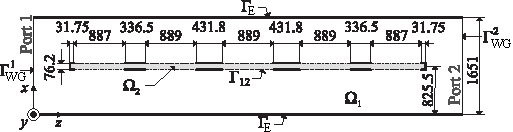
\includegraphics[width=7cm]{bilat}\\
Kerr-type (quadratic) nonlinearity
\begin{equation*}
\tilde{\epsilon}_r(\vec{E}(\vec{r}), \vec{r}) = \bar{\epsilon}_r(\vec{r}) + 
\alpha_2 \ |\vec{E}(\vec{r})|^2, \qquad \vec{r} \in \Omega_2
\end{equation*}
\noindent where $\bar{\epsilon}_r(\vec{r}) = 2.1$ and 
$\alpha_2~=~1.625~10^{-10}~{\frac{\mathrm{m}^2}{\mathrm{V}^2}}$.

}

\frame{
\frametitle{Millimeter-wave bandpass filter with nonlinear dielectrics}
$\text{TE}_{10}$ spectral response for linear (top) and nonlinear 
(bottom) permittivity with $E_i = 10$~$\frac{\text{kV}}{\text{m}}$. The results are compared with Comsol
RF module linear and nonlinear solutions\\[.2cm]
\centering
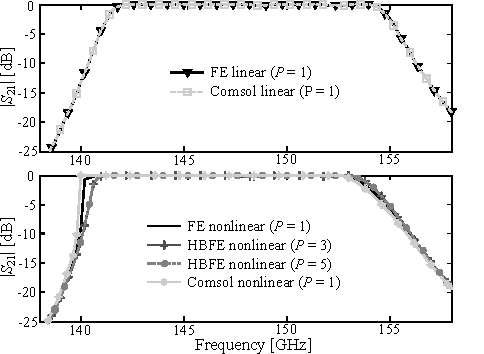
\includegraphics[width=7cm]{spectrumNHarm}

}

\frame{
\frametitle{Millimeter-wave bandpass filter with nonlinear dielectrics}
$|\text{E}_y|$ distribution within the filter at fundamental 
($f_0 =$ 146 ~GHz), $3^\text{rd}$ and $5^\text{th}$ order harmonics 
($\text{E}_i = 10 ~{\frac{\text{kV}}{\text{m}}}$)\\[.2cm]
\centering
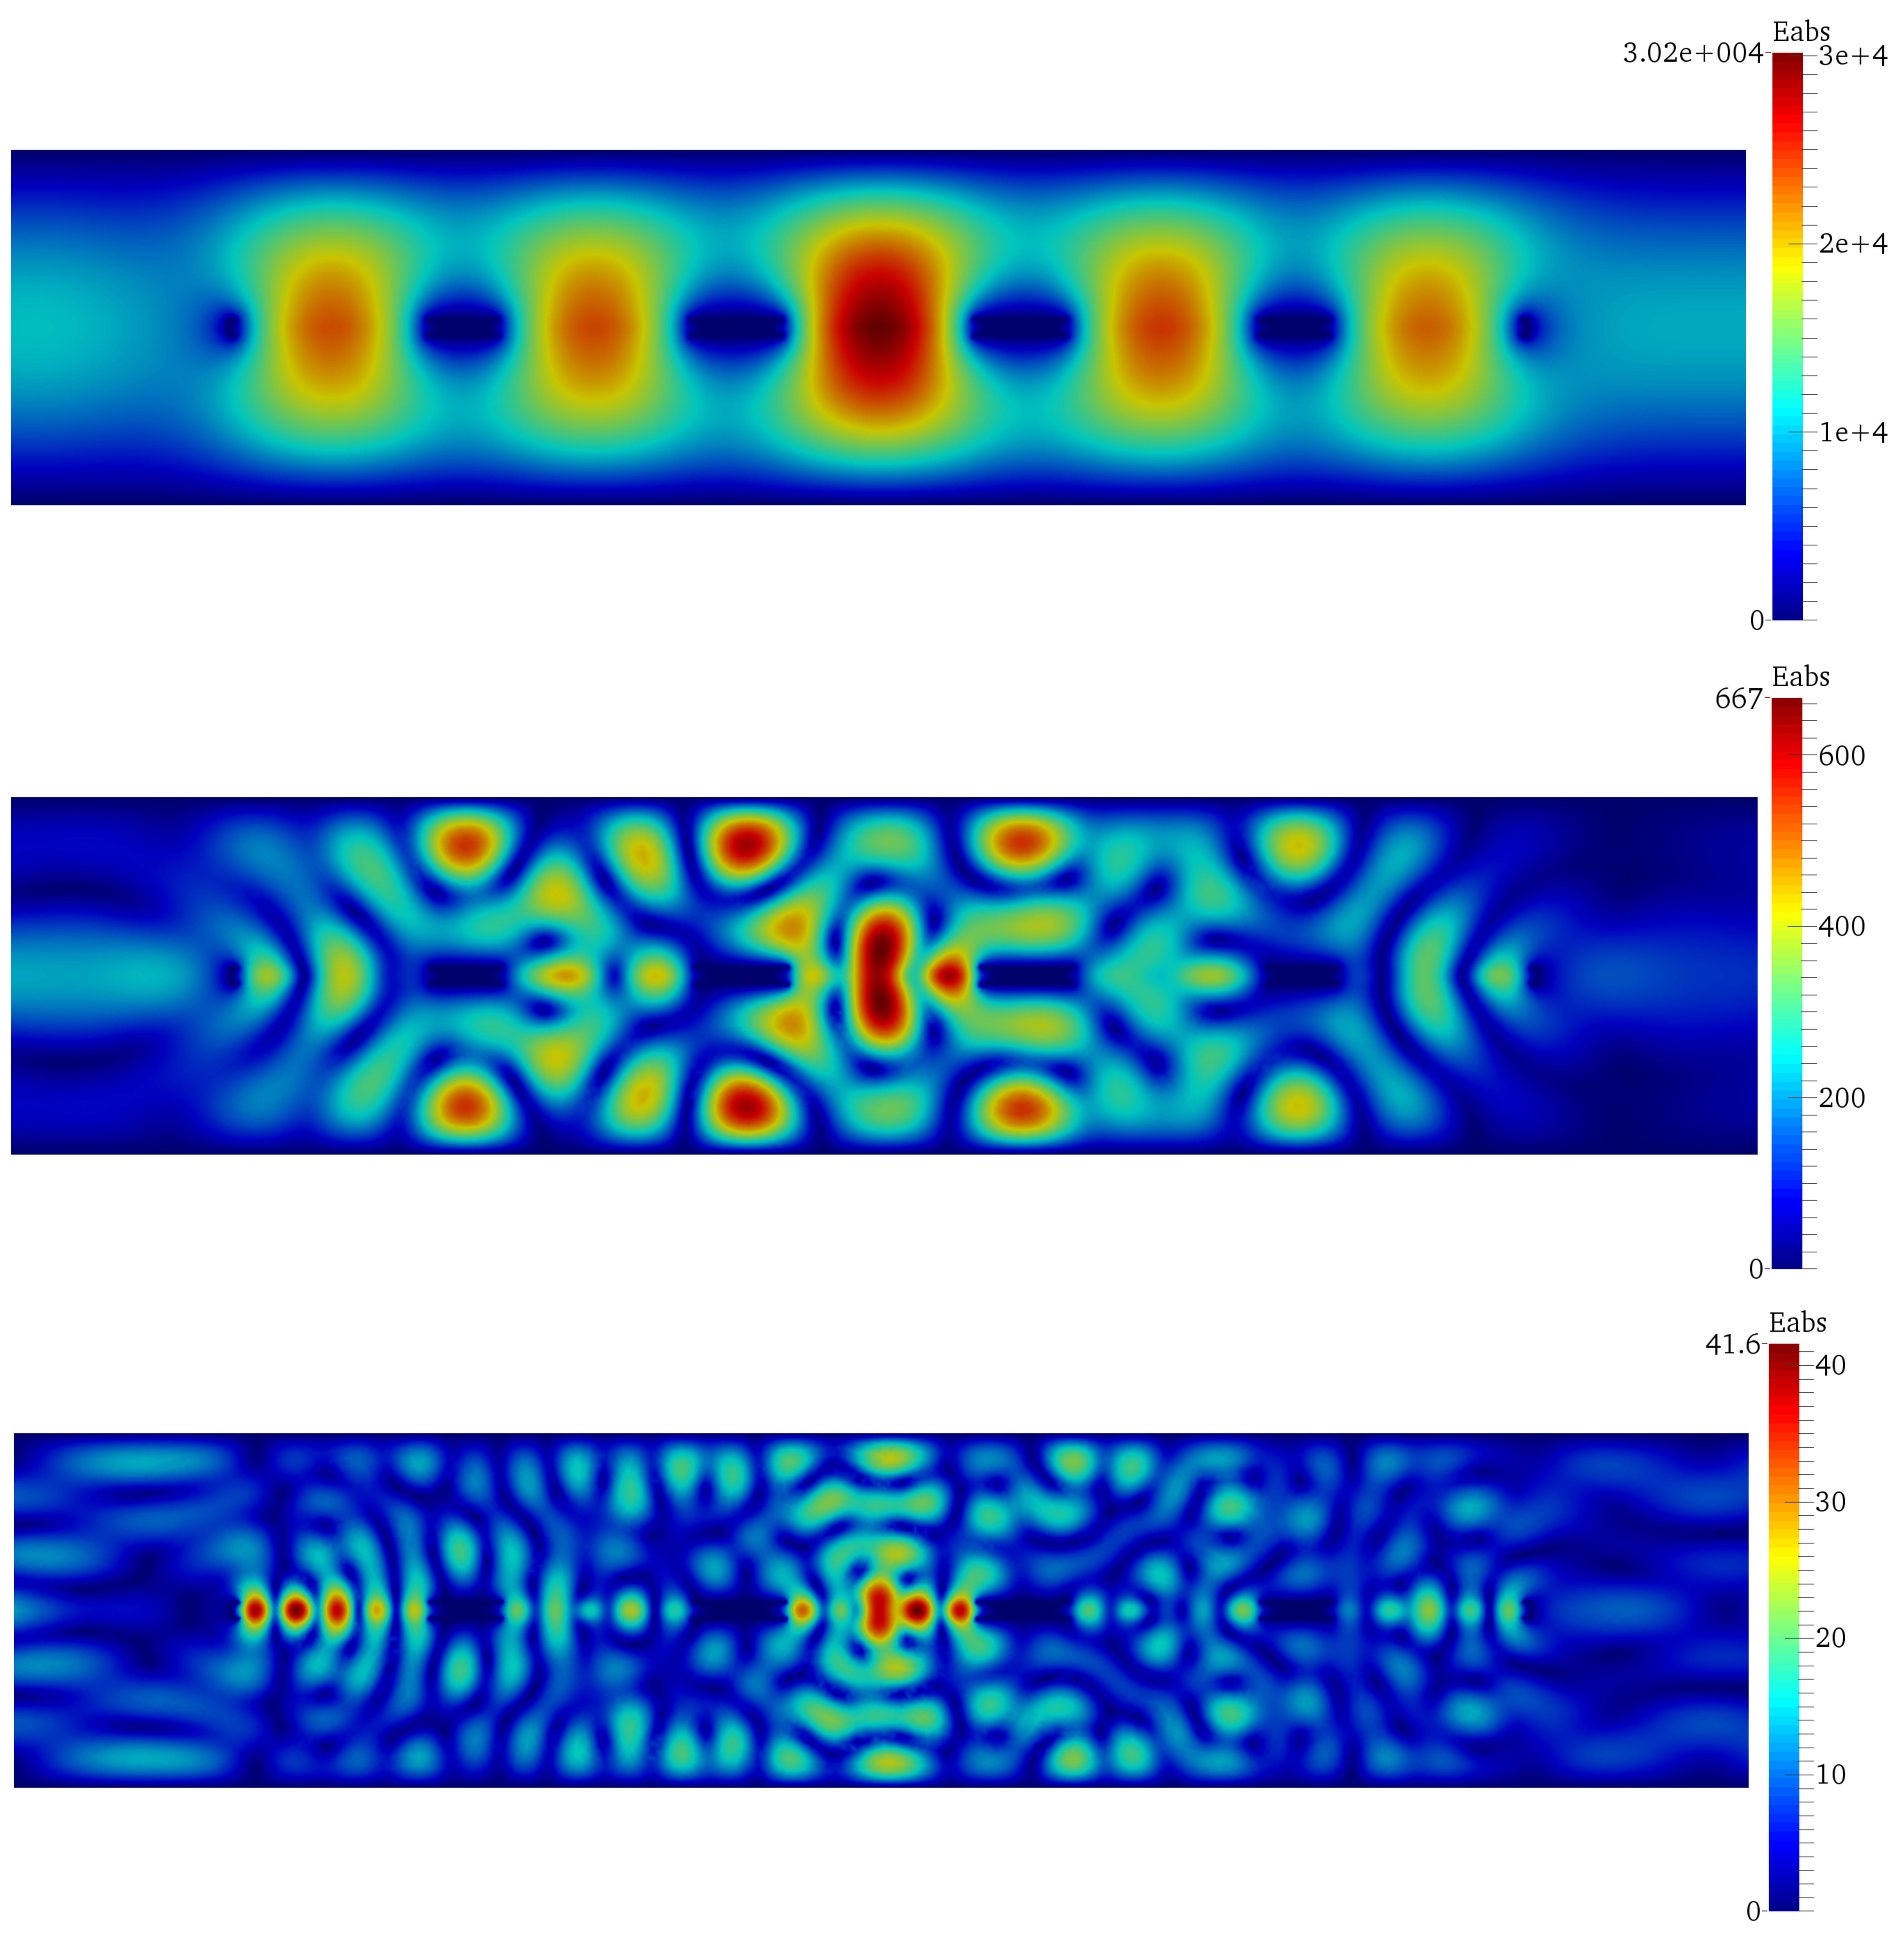
\includegraphics[width=6cm]{FieldsCol}
}

\frame{
\frametitle{Millimeter-wave bandpass filter with nonlinear dielectrics}
$|S_{21}|$ of the nonlinear filter for
several values of $E_i$ compared to the linear case. Field is approximated
up to the $5^\text{th}$ harmonic\\[.2cm]
\centering
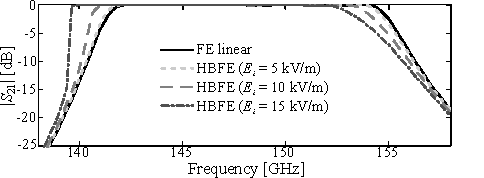
\includegraphics[width=7cm]{spectrumS21b}\\
\begin{itemize}
\item Frequency shift due to an increased permittivity
\end{itemize}
}

\frame{
\frametitle{Millimeter-wave bandpass filter with nonlinear dielectrics}
Relative error of the spectrum at fundamental frequency for various $E_i$ values\\[.2cm]
\centering
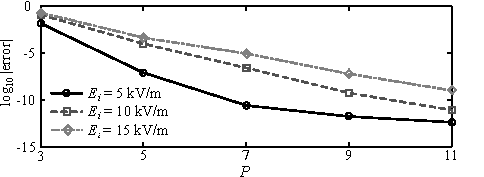
\includegraphics[width=7cm]{convergence}
\begin{itemize}
\item The higher the impinging power, the higher are the required harmonics to retain in the truncated Fourier series
\end{itemize}
}

%\frame{
%\frametitle{Microwave circulator intermodulation products}
%Transverse magnetic field formulation (2D)\\[.2cm]
%\centering
%\begin{columns}
%\begin{column}{.6\textwidth}
%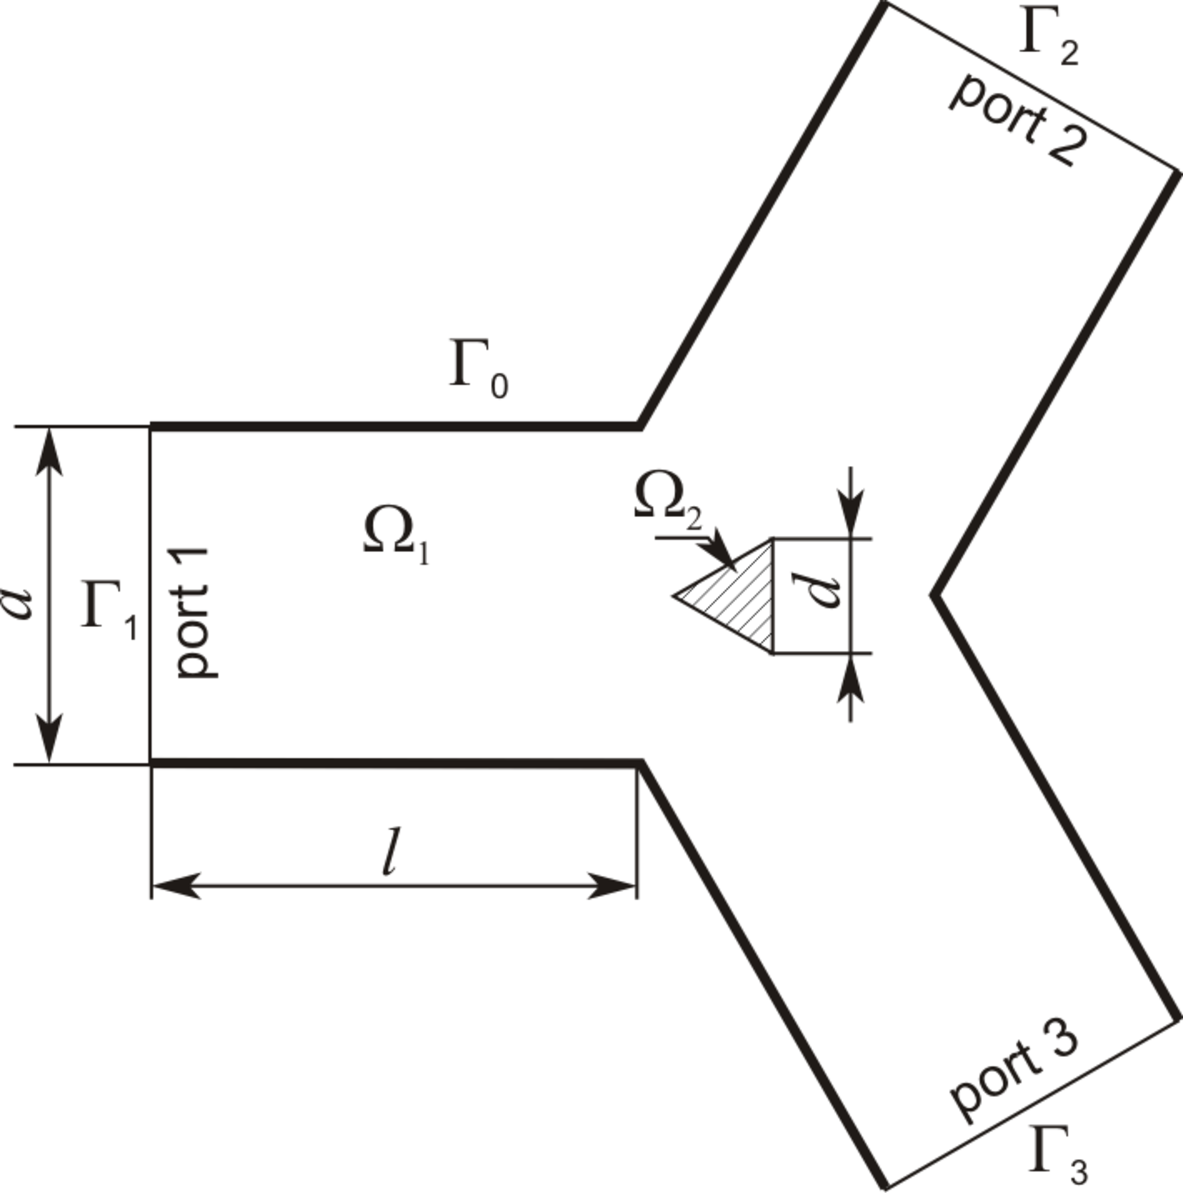
\includegraphics[width=5cm]{Koshiba}
%\end{column}
%\begin{column}{.4\textwidth}
%Ferrite characteristics ($\Omega_2$)
%\begin{gather*}
%\label{eq:ferrite}
%\dyad{\mu}_r = 
%\begin{bmatrix}
%\mu_r& j\kappa_r\\
%-j\kappa_r& \mu_r
%\end{bmatrix}\\
%\dyad{\epsilon}_r = \epsilon_r\\
%\mu_r = 1 + \frac{(\omega_0 + j\omega\alpha)\omega_m}{(\omega_0 + j\omega\alpha)^2-\omega^2}\\
%\kappa_r = \frac{\omega\omega_m}{(\omega_0 + j\omega\alpha)^2-\omega^2}\\
%\omega_0 = \gamma H_i\\ 
%\omega_m = \gamma M_s\\
%\alpha = \gamma \frac{\Delta H}{2\omega}\\
%\end{gather*}
%
%\end{column}
%\end{columns}
%
%
%}
%
%
%\frame{
%\frametitle{Microwave circulator intermodulation products}
%Koshiba et al.\footfullcite{koshiba1986finite}\\[.2cm]
%\centering
%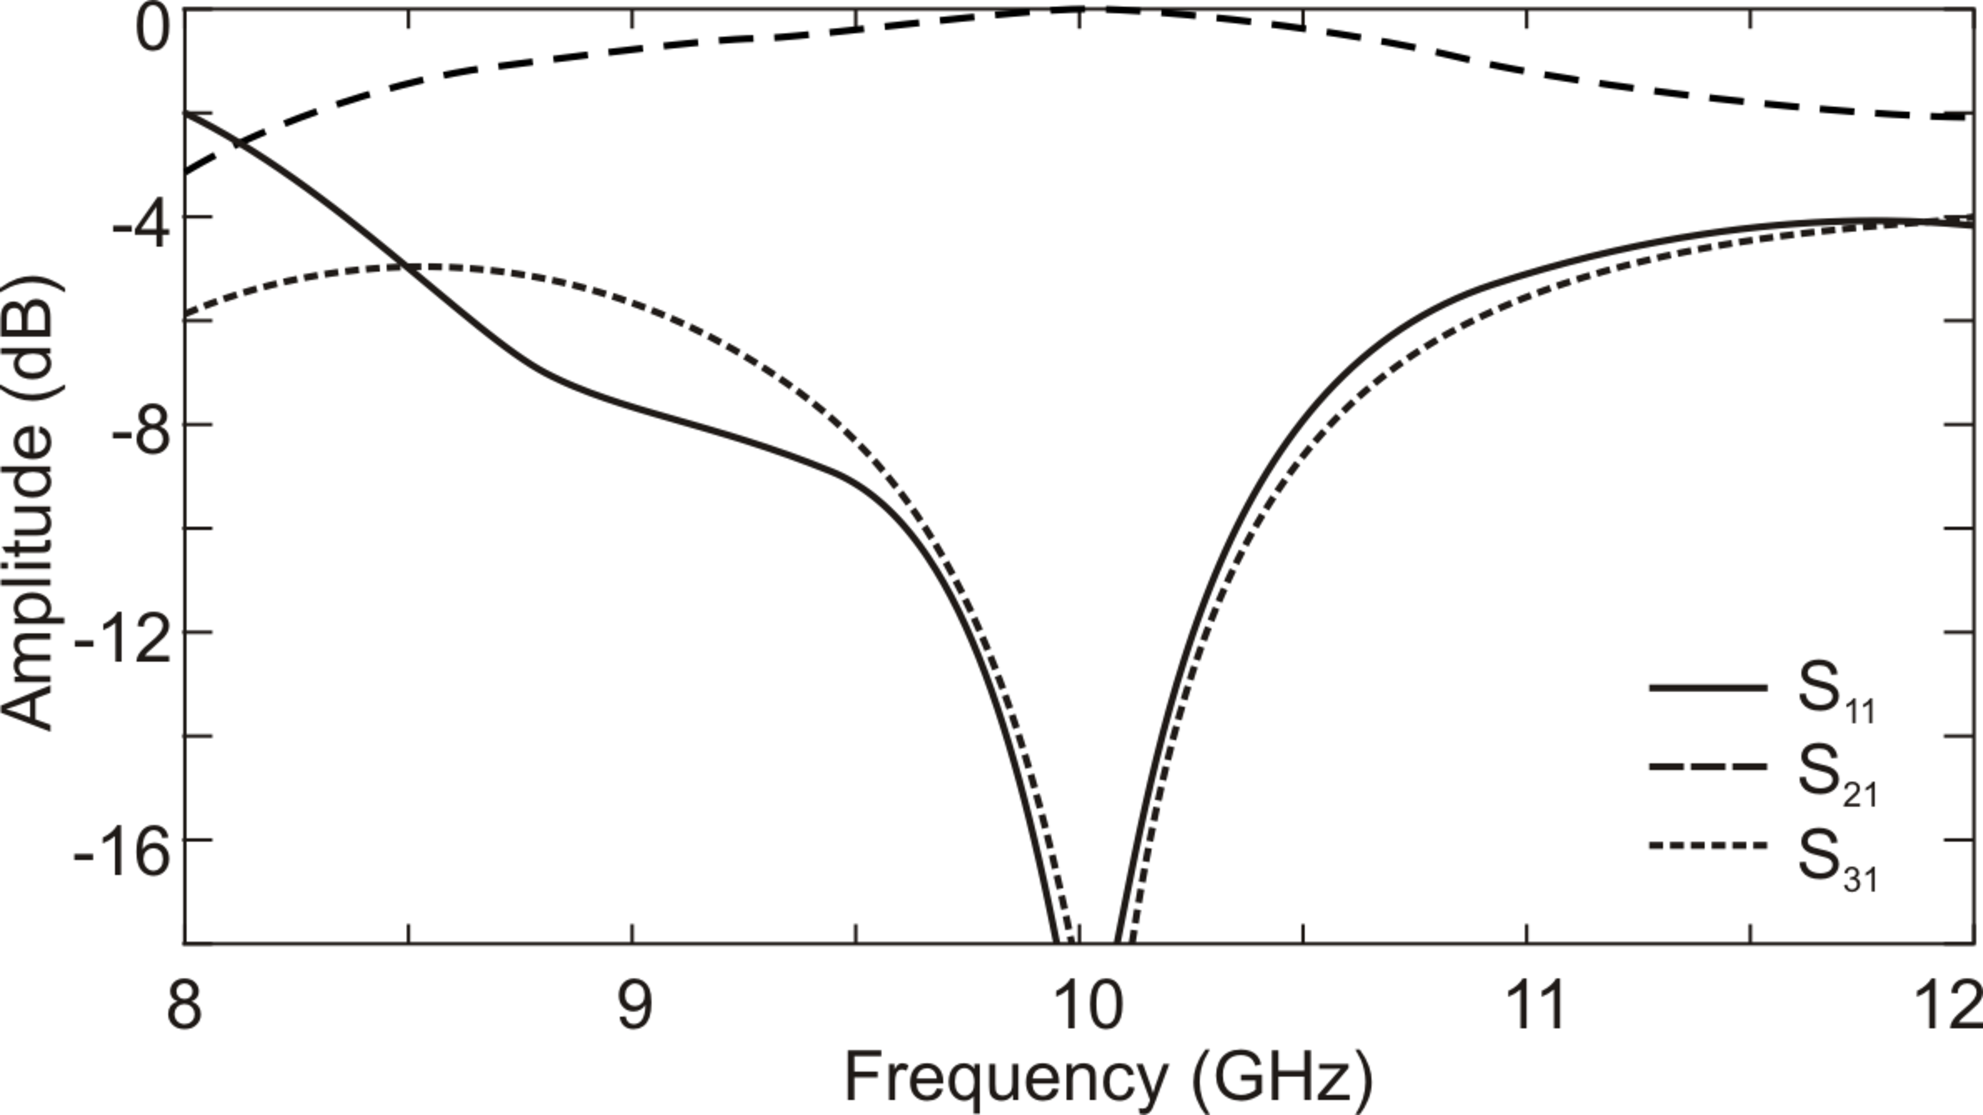
\includegraphics[width=7cm]{circresplin}
%\begin{gather*}
%\gamma = 1.76~10^{7}~ \frac{\text{C}}{\text{kg}}, H_i = 200~\text{G}, M_s = 1317~\text{Oe}, \Delta H = 135~\text{Oe} \cdot \text{s}, \epsilon_r = 11.7 
%\end{gather*}
%
%}

\frame{
\frametitle{Barium strontium titanate thin film coplanar waveguide}
\small
The center conductor of the strip is $w = 20~{\mu}$m with $g = 20~{\mu}$m gaps on both sides and $h_G = 0.3~{\mu}$m of thickness. The thickness of the BST thin-film is $h_F = 400$~nm-thick and that of the LAO substrate is $h_S = 500~{\mu}$m. Dimensions of the box are $W=2$~mm, $H=1$~mm and $L=0.42$~mm \footfullcite{mateu2006measurements}\\[.1cm]
\centering
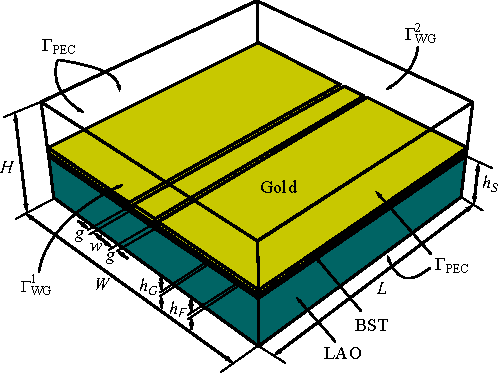
\includegraphics[width=5cm]{CPW}
}

\frame{
\frametitle{Barium strontium titanate thin film coplanar waveguide}
\small
Material properties for the linear CPW\\[.1cm]
\centering
\begin{table}[h!]
\begin{center}
\begin{tabular}{|c|c|c|c|c|} \hline
Material & ${\bar{\epsilon}'}_r$ & $\bar{\mu}_r$ & $\bar{\sigma}~\mat{\frac{\mathrm{S}}{\mathrm{m}}}$ & $\tan \delta = \frac{\bar{\epsilon}''}{\bar{\epsilon}'}$ \\ \hline \hline
LAO & 24 & 1 & 0 & 0 \\ \hline
BST & 475 & 1 & 0 & 0.0842 \\ \hline
Gold & 1 & 0.99996 & $4.1~10^7$ & 0 \\ \hline
Vacuum & 1 & 1 & 0 & 0 \\ \hline
\end{tabular}
\end{center}
\label{tab:CPWmat}
\end{table} 
}

\frame{
\frametitle{Barium strontium titanate thin film coplanar waveguide}
Spectral response of the CPW ($S_{{\text{port1|port2}}_{\text{mode1|mode2}}}$)\\[.1cm]
\centering
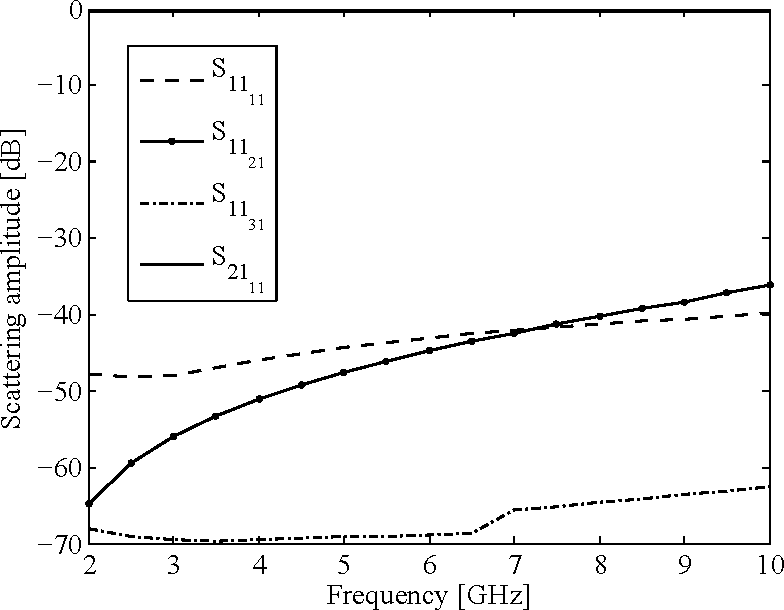
\includegraphics[width=7cm]{CPWlinScat}
}

\frame{
\frametitle{Barium strontium titanate thin film coplanar waveguide}
Coplanar mode traveling through the CPW at 6~GHz\\[.2cm]
\centering
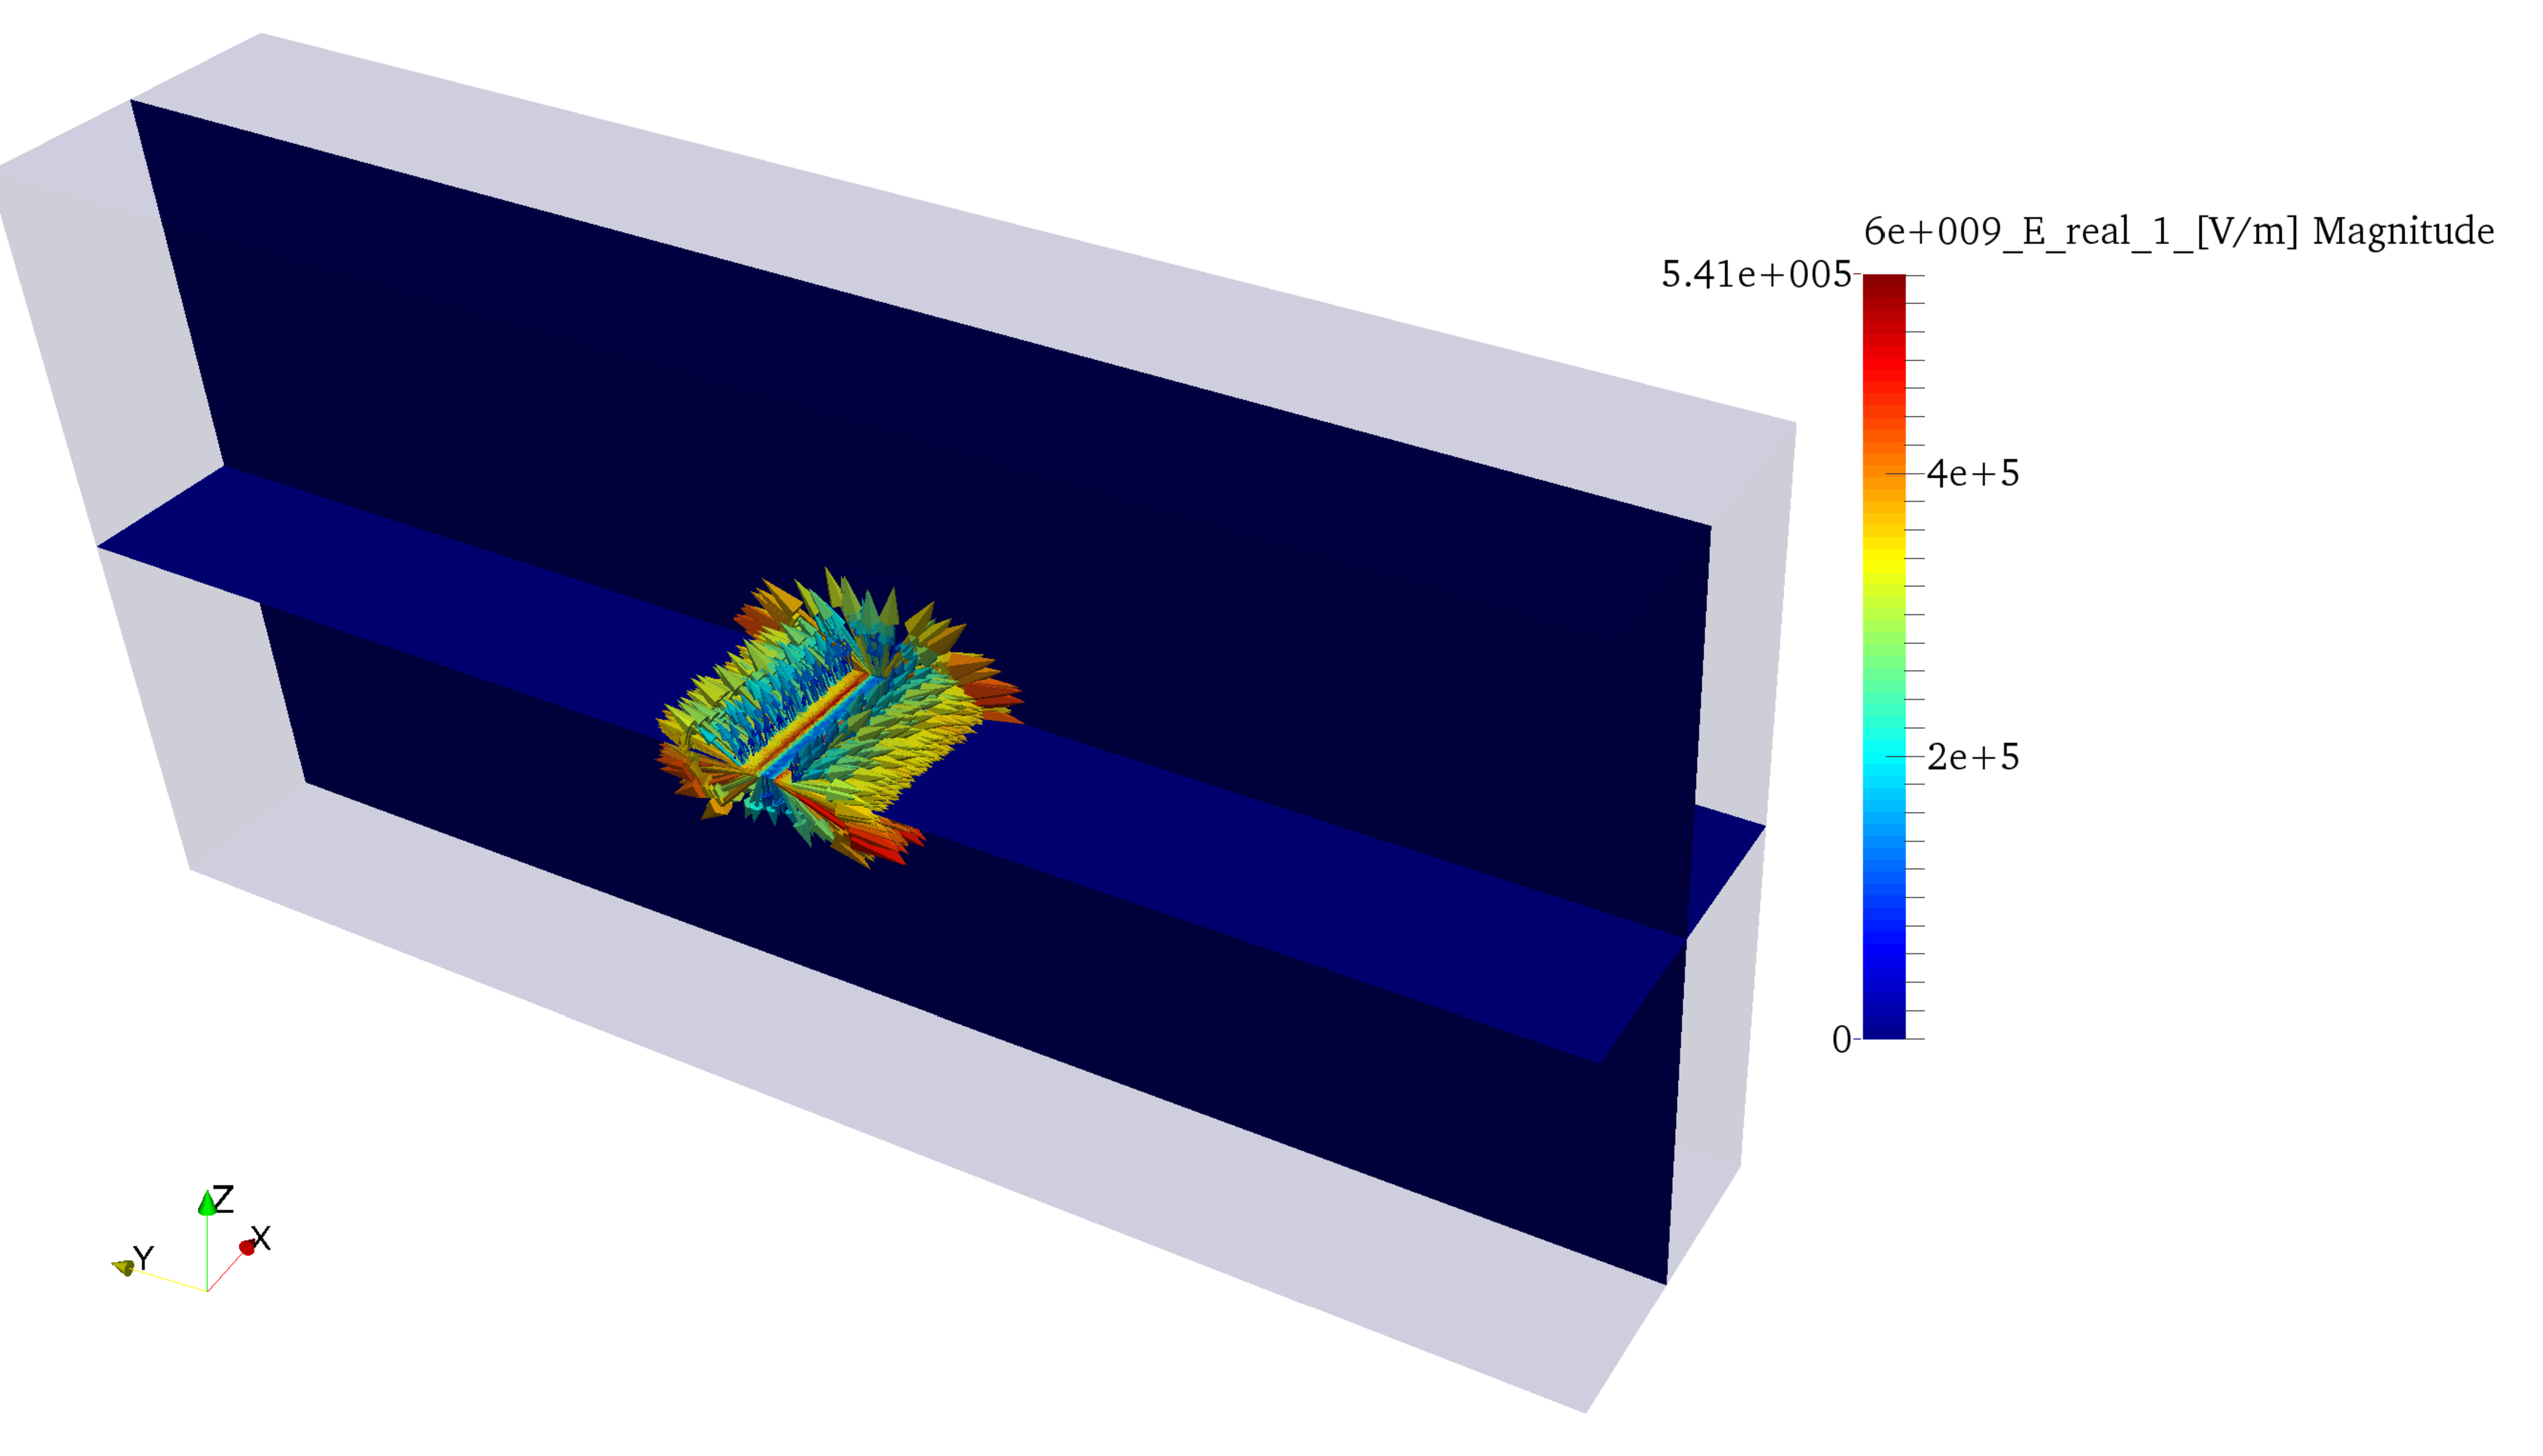
\includegraphics[width=8cm]{CPWlin1}
}

\frame{
\frametitle{Barium strontium titanate thin film coplanar waveguide}
Stripline mode traveling through the CPW at 6~GHz\\[.2cm]
\centering
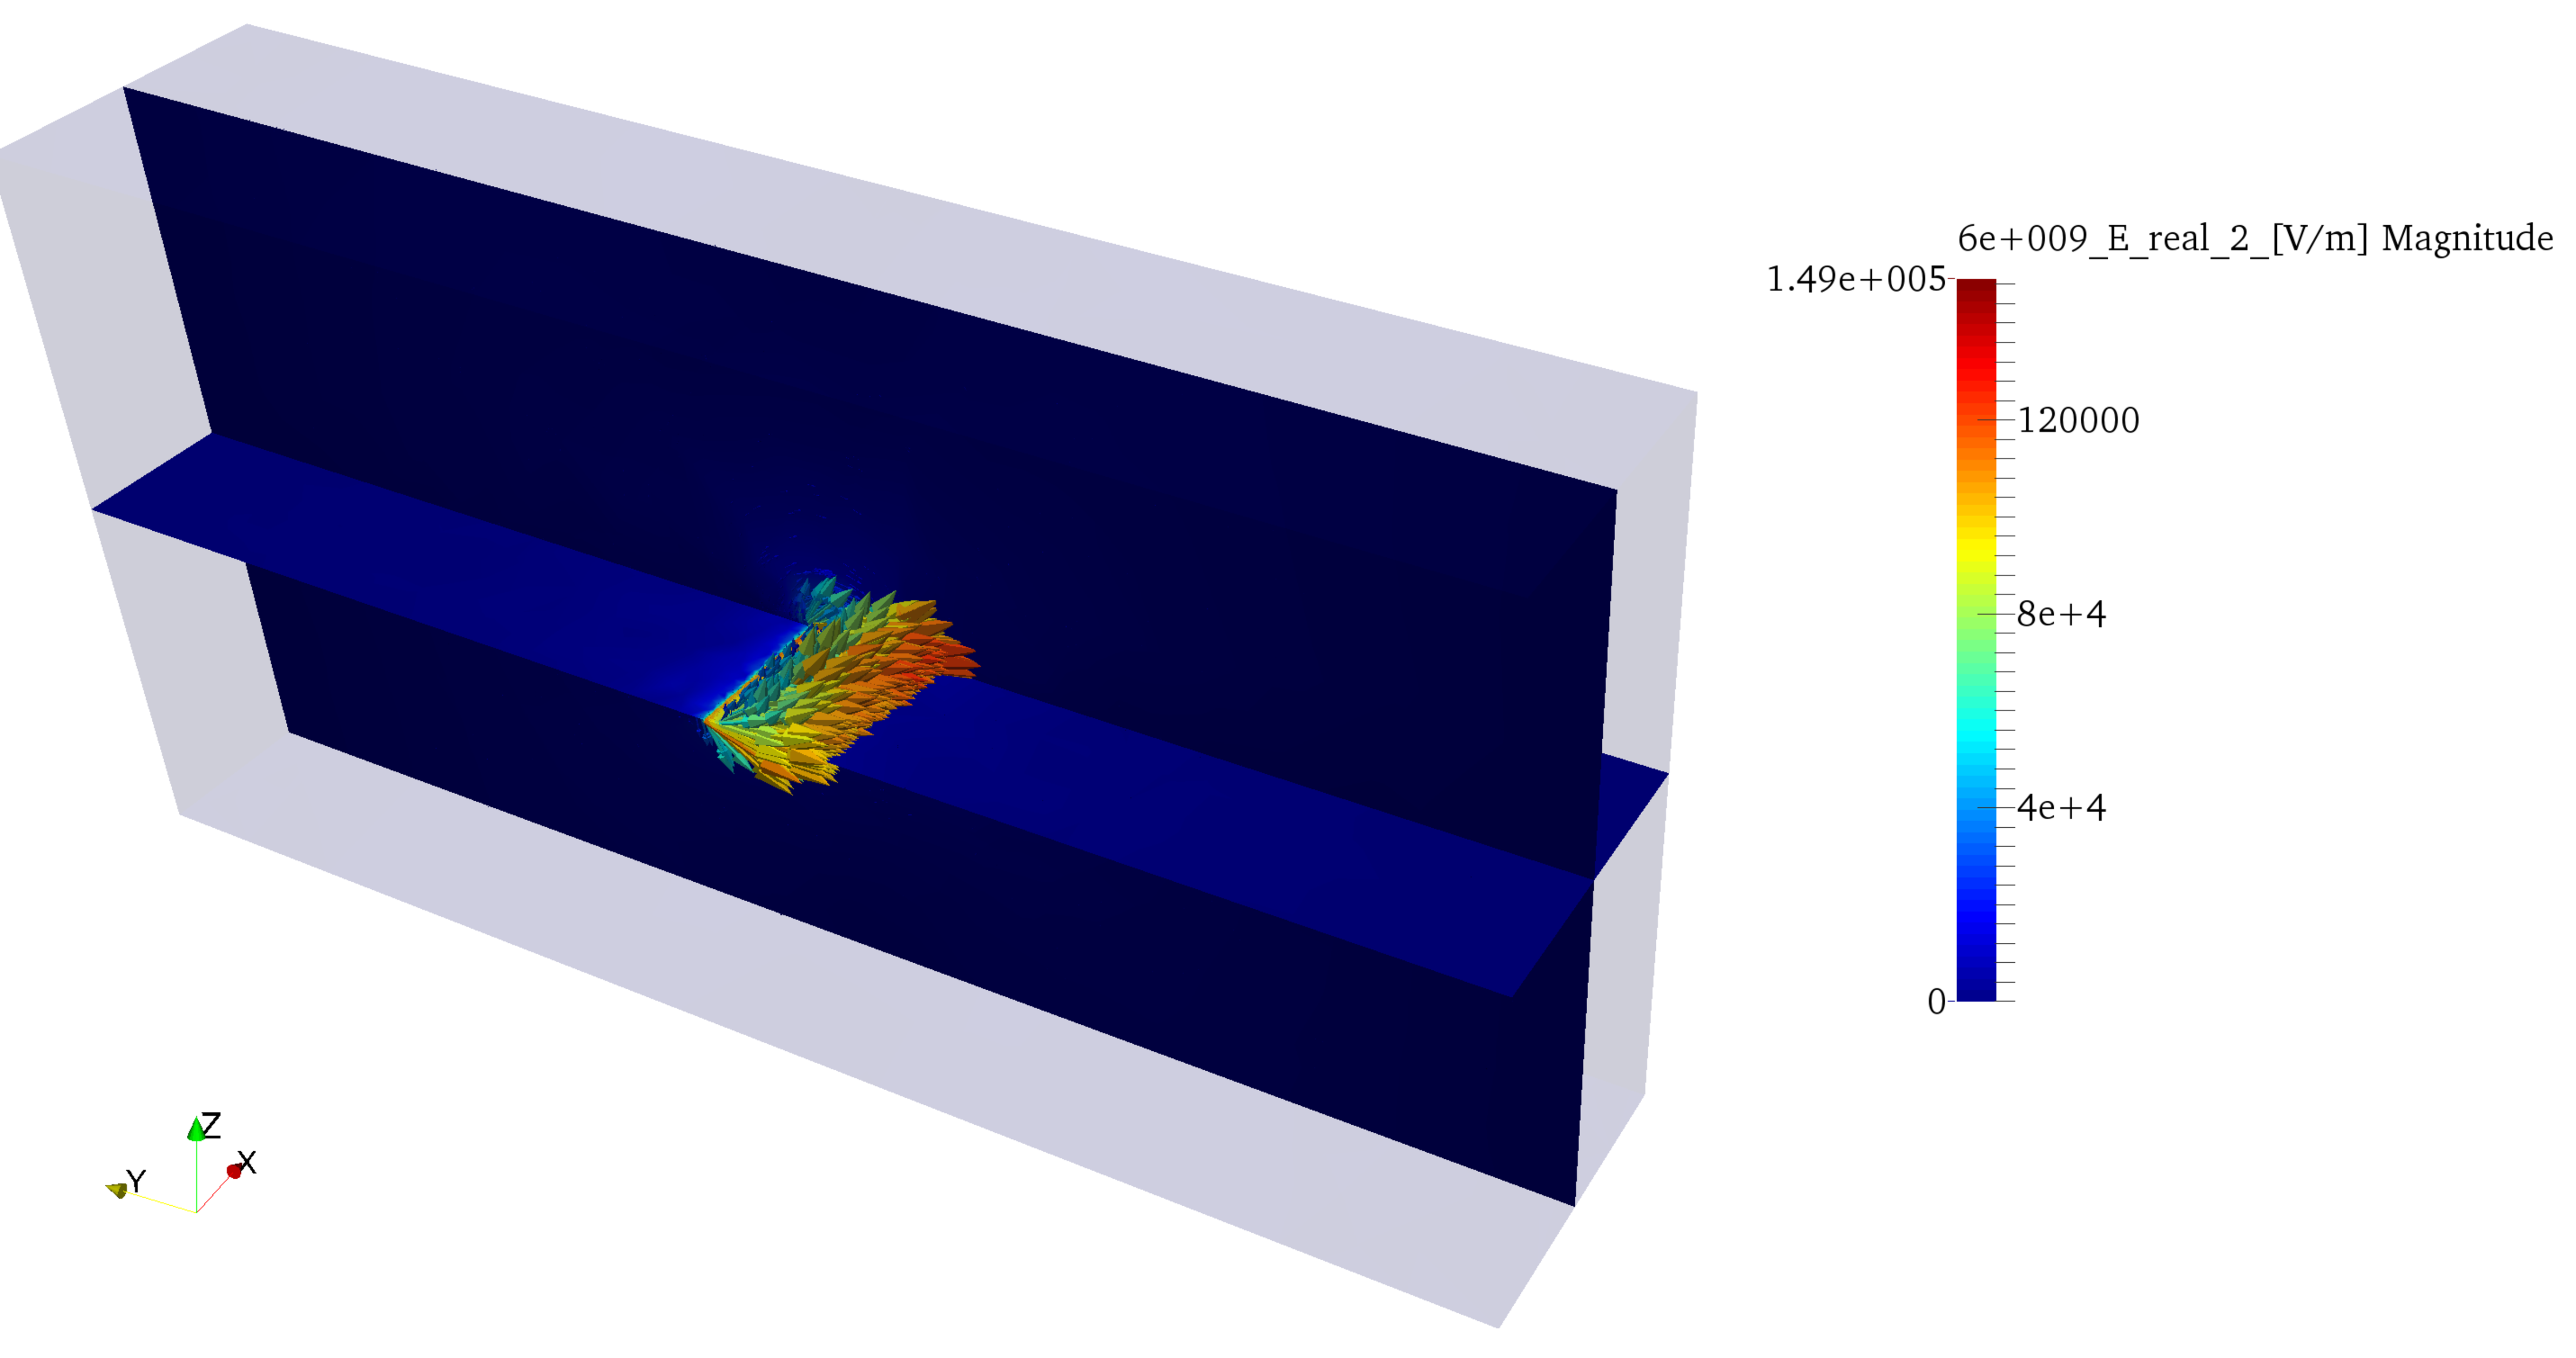
\includegraphics[width=8cm]{CPWlin2}
}

\frame{
\frametitle{Barium strontium titanate thin film coplanar waveguide}
First hibrid TE mode traveling through the CPW at 6~GHz\\[.2cm]
\centering
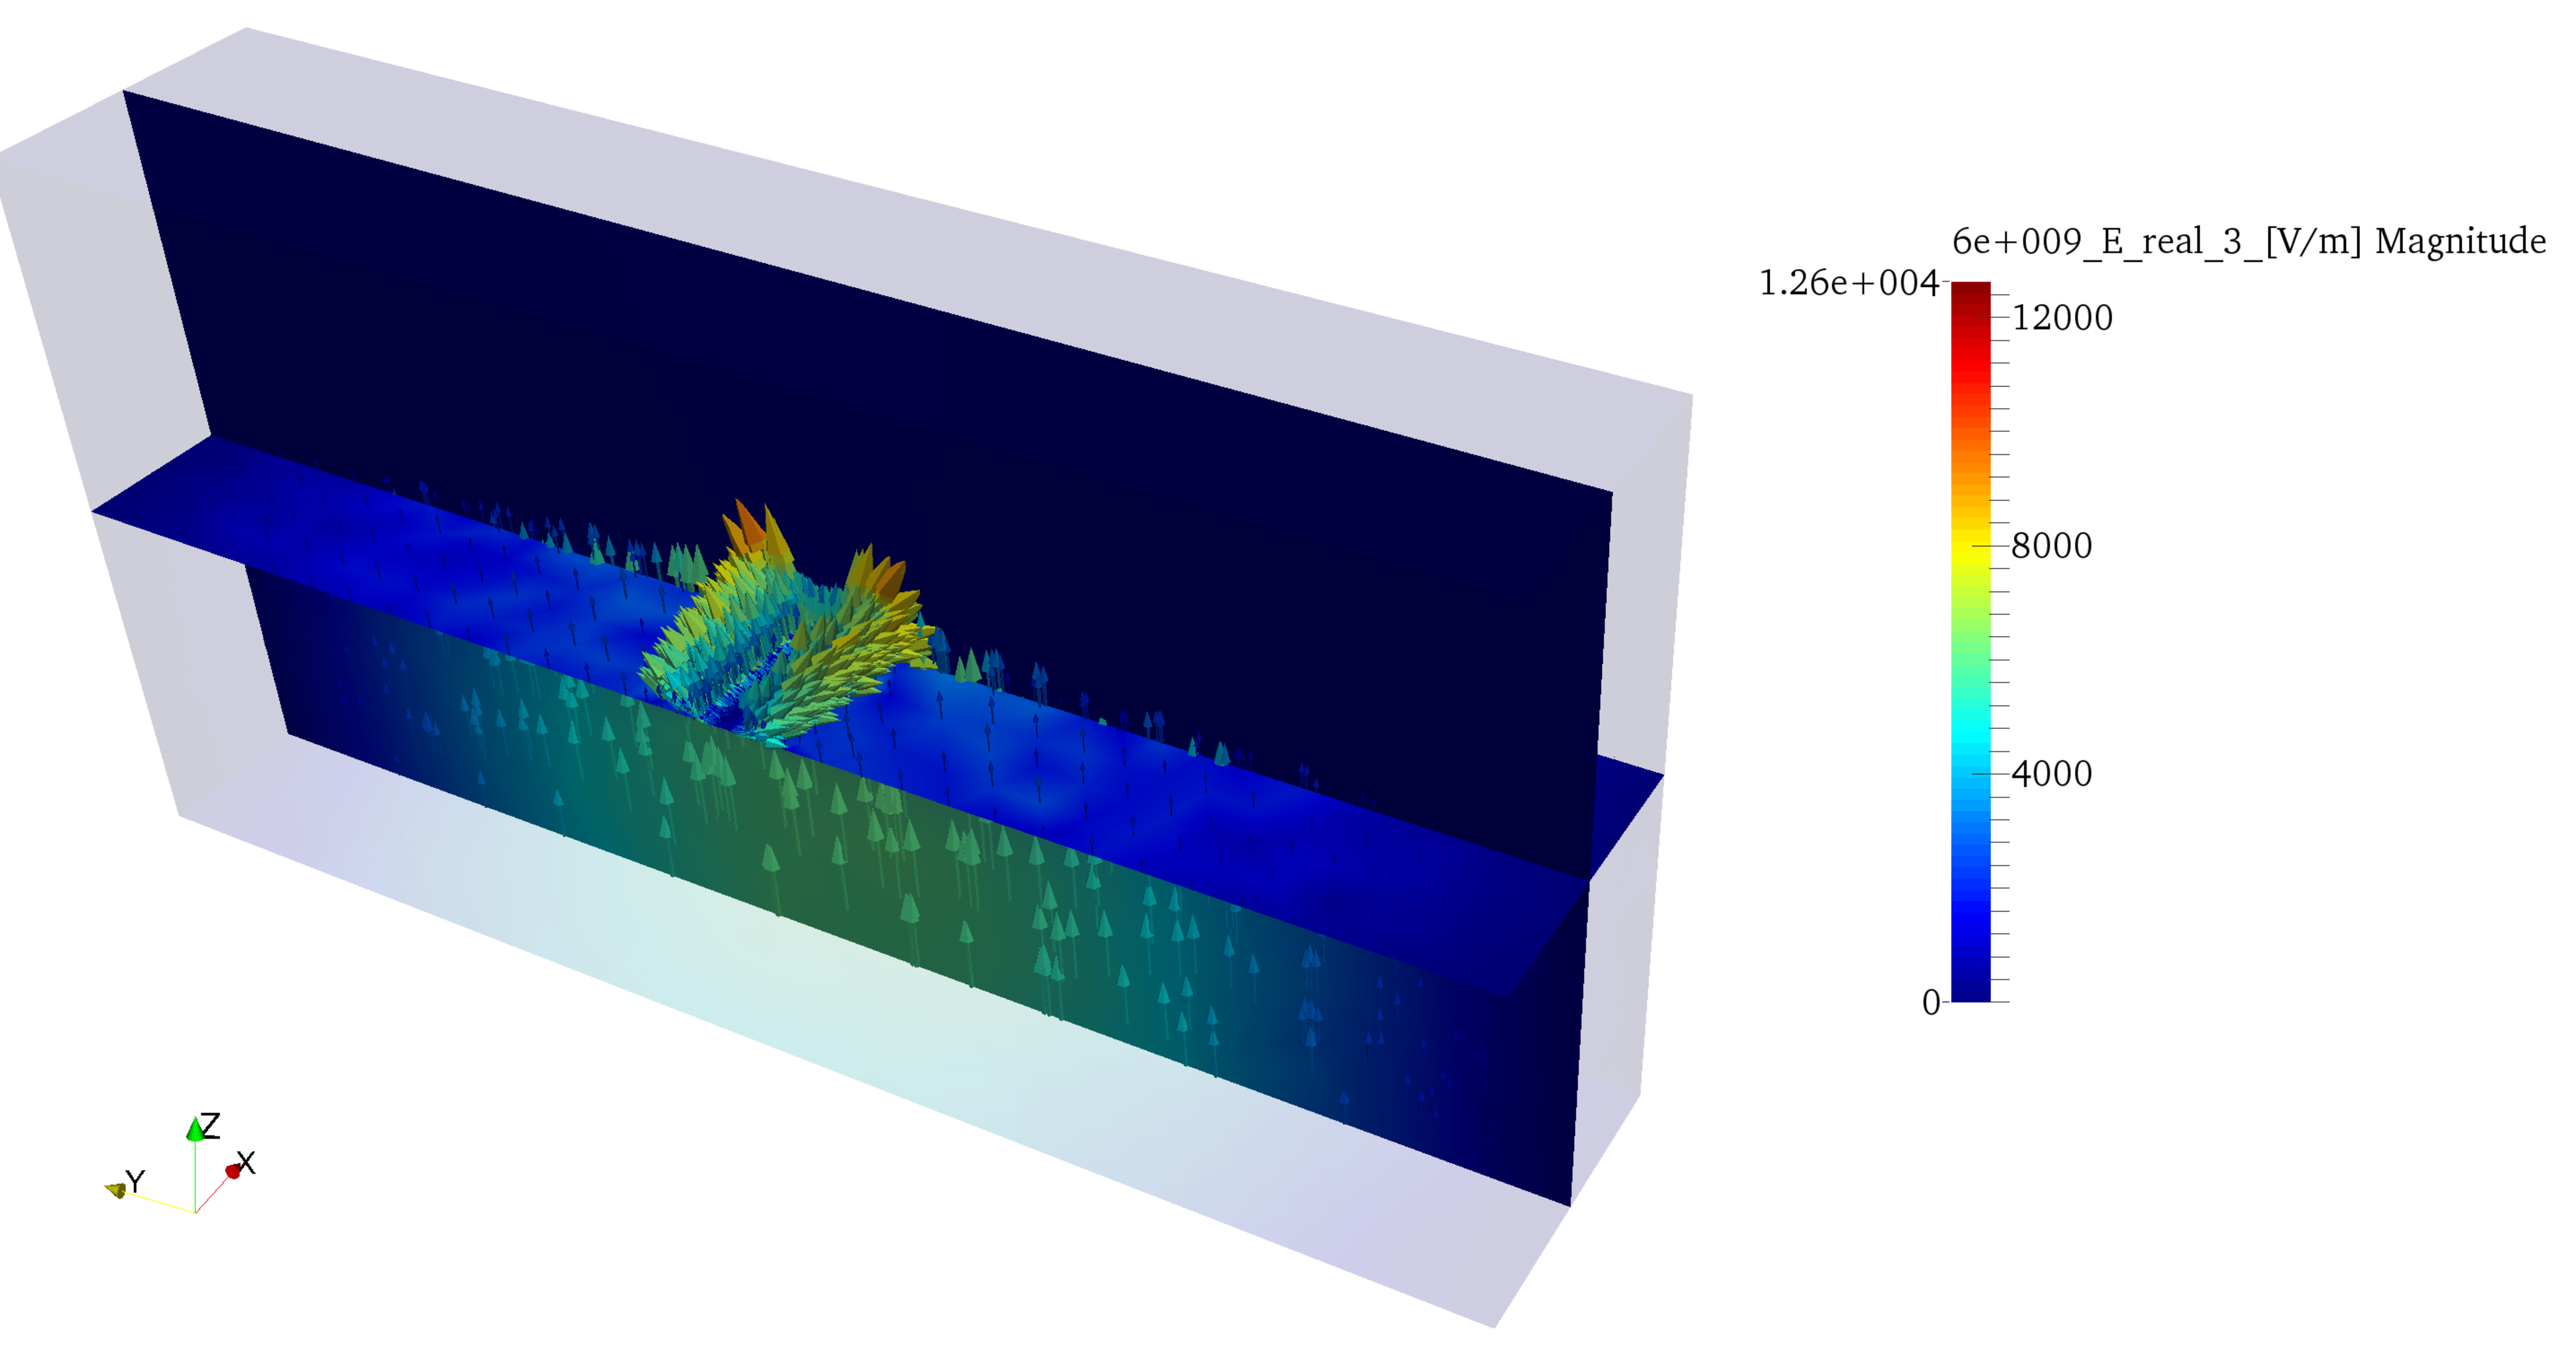
\includegraphics[width=8cm]{CPWlin3}
}

\frame{
\frametitle{Barium strontium titanate thin film coplanar waveguide}
Nonlinear permittivity as measured by Mateu et al.\\[.2cm]
\centering
\begin{equation*}
\tilde{{\varepsilon}'}_r(\mathbf{E}, \mathbf{r}) = {\bar{\varepsilon}'}_r \left( 1 + 
\alpha_2 \ |\mathbf{E}|^2 \right), \qquad \mathbf{r} \in \Omega_2
\end{equation*}
$\alpha_2 = - 5.01~10^{-14}~\frac{\text{m}^2}{\text{V}^2}$
}

\frame{
\frametitle{Barium strontium titanate thin film coplanar waveguide}
Third harmonic spurious power computed with the HBFE. Comparisons are with measurements reported in Mateu et al.\\[.2cm]
\centering
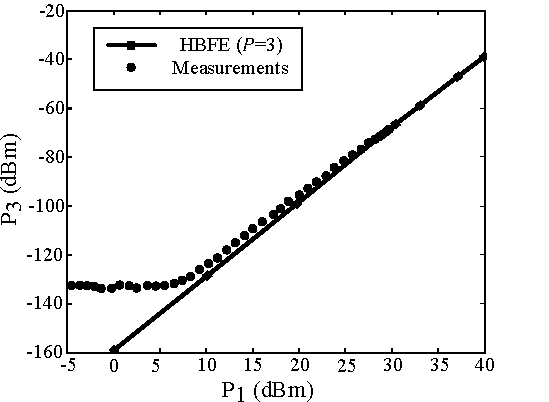
\includegraphics[width=8cm]{P3}
}

\section{Conclusion}
\subsection{Summary}
\frame{
\frametitle{Summary}
\begin{itemize}
\item A conventional finite element sofware has been implemented, based on several electromagnetic problems formulations. Validation of the code is performed through rigorous comparison with commercial packages (previously validated through experiements)
\item In the quest of a domain decomposition method to enable large problems analysis, several formulations have been tested and their performances evaluated. A GMRES($r$) solver, FETI-DP based Gauss-Seidel preconditioner has been individuated as a very promising solver
\item The harmonic balance finite element method has been applyed to the wave equation. Its performance and accuracy have been analyzed. HBFE results to be a promising method for full-wave electromagnetic modeling of nonlinear permittivity materials
\end{itemize}
}

\subsection{Outlook}
\frame{
\frametitle{Outlook}
\begin{itemize}
\item The edge corners problem in DD preconditioned solvers still have to be investigated 
\item It has been noticed, during the development of Schur based DD preconditioner that the substitution of $\mat{A_{\Gamma\Gamma}} \leftarrow \mat{S}$  leads to very fast convergence (2 iterations). Approximate Schur complement matrices should be investigated
\item HBFE method should be extended to optical frequencies analyzes, where harmonic generation is a matter of strong interest
\end{itemize}
}

\frame{
\frametitle{List of Pubblications}
\scriptsize
\textbf{Refereed papers}
\begin{enumerate}
\item  L. Ntibarikure, G. Pelosi, S. Selleri, ``Efficient harmonic balance analysis of waveguide devices with nonlinear dielectrics,'' \emph{Microwave and Wireless Components Letters, IEEE}, vol. 22, no. 5, pp. 221--223, 2012.
\item  L. Ntibarikure, G. Pelosi, S. Selleri, ``Harmonic balance domain decomposition finite elements for nonlinear passive microwave devices analysis,'' \emph{Special Issue on \quotes{Finite Elements for Microwave Engineering}, Electromagnetics}, vol.~34, no. 3, 2014.
\end{enumerate}

\textbf{Conference proceedings} 
\begin{enumerate}
\item  L. Ntibarikure, ``Model order reduction in finite element analysis of phased array antennas,'' in \emph{Numero Speciale 8 - Serie di Elettromagnetismo su \quotes{XIX Riunione Nazionale di Elettromagnetismo (RiNEm)}, Atti della \quotes{Fondazione Giorgio Ronchi}}, vol. LXVIII, no. 4, pp. 97--102, 2012. \underline{Barzilai prize}
\end{enumerate}


\textbf{Conferences}
\begin{enumerate}
\item L. Ntibarikure, G. Pelosi, and S. Selleri, ``Harmonic balance domain decomposition finite element for nonlinear passive microwave devices analysis,'' in \emph{11th International Workshop on Finite Elements for Microwave Engineering -- FEM2012}, Estes Park, Colorado, USA, Jun. 4--6, 2012.
\item L. Ntibarikure, G. Pelosi, S. Selleri, ``Harmonic balance finite element analysis of third order intermodulation products in ferrite devices,'' in \emph{XIX Riunione Nazionale di Elettromagnetismo -- XIX~RiNEm}, Rome, Italy, Sep. 10--14, 2012.
\item  L. Ntibarikure, ``Model order reduction in finite element analysis of phased array antennas,'' in \emph{XIX Riunione Nazionale di Elettromagnetismo -- XIX~RiNEm}, Rome, Italy, Sep. 10-14, 2012.
\end{enumerate}
}

\end{document}
